\documentclass{amsart}[12pt]
\usepackage{graphicx}
\usepackage{comment}
\usepackage{amscd,mathabx}
\usepackage{amssymb,setspace}
\usepackage{tikz-cd}
\usepackage{latexsym,amsfonts,amssymb,amsthm,amsmath,amscd,stmaryrd,mathrsfs,xcolor}
\usepackage[all, knot]{xy}
\usepackage[top=1in, bottom=1in, left=1in, right=1in]{geometry}
\xyoption{all}
\xyoption{arc}
\usepackage{hyperref}


%\usepackage[notcite,notref]{showkeys}
 
%\CompileMatricesx
\newcommand{\edit}[1]{\marginpar{\footnotesize{#1}}}
%\newcommand{\edit}[1]{}
\newcommand{\rperf}[2]{\operatorname{RPerf}(#1 \into #2)}



\newcommand{\vectwo}[2]{\begin{bmatrix} #1 \\ #2 \end{bmatrix}}

\newcommand{\vecfour}[4]{\begin{bmatrix} #1 \\ #2 \\ #3 \\ #4 \end{bmatrix}}

\newcommand{\Cat}[1]{\left<\left< \text{#1} \right>\right>}


\def\htpy{\simeq_{\mathrm{htpc}}}
\def\tor{\text{ or }}
\def\fg{finitely generated~}

\def\Ass{\operatorname{Ass}}
\def\ann{\operatorname{ann}}
\def\sign{\operatorname{sign}}

\newcommand{\Tor}{\mathrm{Tor}}
\newcommand{\can}{\mathrm{can}}

\def\ob{{\mathfrak{ob}} }
\def\BiAdd{\operatorname{BiAdd}}
\def\BiLin{\operatorname{BiLin}}

\def\Syl{\operatorname{Syl}}
\def\span{\operatorname{span}}

\def\sdp{\rtimes}
\def\cL{\mathcal L}
\def\cR{\mathcal R}



\def\ay{??}
\def\Aut{\operatorname{Aut}}
\def\End{\operatorname{End}}
\def\Mat{\operatorname{Mat}}


\def\a{\alpha}



\def\etale{\'etale~}
\def\tW{\tilde{W}}
\def\tH{\tilde{H}}
\def\tC{\tilde{C}}
\def\tS{\tilde{S}}
\def\tX{\tilde{X}}
\def\tZ{\tilde{Z}}
\def\HBM{H^{\text{BM}}}
\def\tHBM{\tilde{H}^{\text{BM}}}
\def\Hc{H_{\text{c}}}
\def\Hs{H_{\text{sing}}}
\def\cHs{{\mathcal H}_{\text{sing}}}
\def\sing{{\text{sing}}}
\def\Hms{H^{\text{sing}}}
\def\Hm{\Hms}
\def\tHms{\tilde{H}^{\text{sing}}}
\def\Grass{\operatorname{Grass}}
\def\image{\operatorname{im}}
\def\im{\image}
\def\ker{\operatorname{ker}}
\def\coker{\operatorname{coker}}
\def\cone{\operatorname{cone}}
\newcommand{\Hom}{\mathrm{Hom}}

\newcommand{\onto}{\twoheadrightarrow}


\def\ku{ku}
\def\bbu{\bf bu}
\def\KR{K{\mathbb R}}

\def\CW{\underline{CW}}
\def\cP{\mathcal P}
\def\cE{\mathcal E}
\def\cL{\mathcal L}
\def\cJ{\mathcal J}
\def\cJmor{\cJ^\mor}
\def\ctJ{\tilde{\mathcal J}}
\def\tPhi{\tilde{\Phi}}
\def\cA{\mathcal A}
\def\cB{\mathcal B}
\def\cC{\mathcal C}
\def\cZ{\mathcal Z}
\def\cD{\mathcal D}
\def\cF{\mathcal F}
\def\cG{\mathcal G}
\def\cO{\mathcal O}
%\def\cI{\mathcal I}
\def\cS{\mathcal S}
\def\cT{\mathcal T}
\def\cM{\mathcal M}
\def\cN{\mathcal N}
\def\cMpc{{\mathcal M}_{pc}}
\def\cMpctf{{\mathcal M}_{pctf}}
\def\L{\Lambda}

\def\sA{\mathscr A}
\def\sB{\mathscr B}
\def\sC{\mathscr C}
\def\sZ{\mathscr  Z}
\def\sD{\mathscr  D}
\def\sF{\mathscr  F}
\def\sG{\mathscr G}
\def\sO{\mathscr  O}
\def\sI{\mathscr I}
\def\sS{\mathscr S}
\def\sT{\mathscr  T}
\def\sM{\mathscr M}
\def\sN{\mathscr N}

%\newcommand{\inc}{\subseteq}
\newcommand{\id}{\mathrm{id}}


\newcommand{\Aug}[1]{\textcolor{violet}{Lecture of August #1, 2021}}
\newcommand{\Sept}[1]{\textcolor{violet}{Lecture of September #1, 2021}}
\newcommand{\Oct}[1]{\textcolor{violet}{Lecture of October #1, 2021}}
\newcommand{\Nov}[1]{\textcolor{violet}{Lecture of November #1, 2021}}
\newcommand{\Dec}[1]{\textcolor{violet}{Lecture of December #1, 2021}}

\def\Ext{\operatorname{Ext}}
 \def\ext{\operatorname{ext}}



\def\ov#1{{\overline{#1}}}

\def\vecthree#1#2#3{\begin{bmatrix} #1 \\ #2 \\ #3 \end{bmatrix}}

\def\tOmega{\tilde{\Omega}}
\def\tDelta{\tilde{\Delta}}
\def\tSigma{\tilde{\Sigma}}
\def\tsigma{\tilde{\sigma}}


\def\d{\delta}
\def\td{\tilde{\delta}}

\def\e{\epsilon}
\def\nsg{\unlhd}
\def\pnsg{\lhd}

\newcommand{\tensor}{\otimes}
\newcommand{\homotopic}{\simeq}
\newcommand{\homeq}{\cong}
\newcommand{\iso}{\approx}

\DeclareMathOperator{\ho}{Ho}
\DeclareMathOperator*{\colim}{colim}


\newcommand{\Q}{\mathbb{Q}}
\renewcommand{\H}{\mathbb{H}}

\newcommand{\bP}{\mathbb{P}}
\newcommand{\bM}{\mathbb{M}}
\newcommand{\A}{\mathbb{A}}
\newcommand{\bH}{{\mathbb{H}}}
\newcommand{\G}{\mathbb{G}}
\newcommand{\bR}{{\mathbb{R}}}
\newcommand{\bL}{{\mathbb{L}}}
\newcommand{\R}{{\mathbb{R}}}
\newcommand{\F}{\mathbb{F}}
\newcommand{\E}{\mathbb{E}}
\newcommand{\bF}{\mathbb{F}}
\newcommand{\bE}{\mathbb{E}}
\newcommand{\bK}{\mathbb{K}}


\newcommand{\bD}{\mathbb{D}}
\newcommand{\bS}{\mathbb{S}}

\newcommand{\bN}{\mathbb{N}}


\newcommand{\bG}{\mathbb{G}}

\newcommand{\C}{\mathbb{C}}
\newcommand{\Z}{\mathbb{Z}}
\newcommand{\N}{\mathbb{N}}

\newcommand{\M}{\mathcal{M}}
\newcommand{\W}{\mathcal{W}}



\newcommand{\itilde}{\tilde{\imath}}
\newcommand{\jtilde}{\tilde{\jmath}}
\newcommand{\ihat}{\hat{\imath}}
\newcommand{\jhat}{\hat{\jmath}}

\newcommand{\fc}{{\mathfrak c}}
\newcommand{\fp}{{\mathfrak p}}
\newcommand{\fm}{{\mathfrak m}}
\newcommand{\fn}{{\mathfrak n}}
\newcommand{\fq}{{\mathfrak q}}

\newcommand{\op}{\mathrm{op}}
\newcommand{\dual}{\vee}

\newcommand{\DEF}[1]{\emph{#1}\index{#1}}
\newcommand{\Def}[1]{#1 \index{#1}}


% The following causes equations to be numbered within sections
\numberwithin{equation}{section}


\theoremstyle{plain} %% This is the default, anyway
\newtheorem{thm}[equation]{Theorem}
\newtheorem{thmdef}[equation]{TheoremDefinition}
\newtheorem{introthm}{Theorem}
\newtheorem{introcor}[introthm]{Corollary}
\newtheorem*{introthm*}{Theorem}
\newtheorem{question}{Question}
\newtheorem{cor}[equation]{Corollary}
\newtheorem{por}[equation]{Porism}
\newtheorem{lem}[equation]{Lemma}
\newtheorem{lemminition}[equation]{Lemminition}
\newtheorem{prop}[equation]{Proposition}
\newtheorem{porism}[equation]{Porism}
\newtheorem{fact}[equation]{Fact}


\newtheorem{conj}[equation]{Conjecture}
\newtheorem{quest}[equation]{Question}

\theoremstyle{definition}
\newtheorem{defn}[equation]{Definition}
\newtheorem{chunk}[equation]{}
\newtheorem{ex}[equation]{Example}

\newtheorem{exer}[equation]{Optional Exercise}

\theoremstyle{remark}
\newtheorem{rem}[equation]{Remark}

\newtheorem{notation}[equation]{Notation}
\newtheorem{terminology}[equation]{Terminology}



\renewcommand{\sec}[1]{\section{#1}}
\newcommand{\ssec}[1]{\subsection{#1}}
\newcommand{\sssec}[1]{\subsubsection{#1}}

\newcommand{\br}[1]{\lbrace \, #1 \, \rbrace}
\newcommand{\li}{ < \infty}
\newcommand{\quis}{\simeq}
\newcommand{\xra}[1]{\xrightarrow{#1}}
\newcommand{\xla}[1]{\xleftarrow{#1}}
\newcommand{\xlra}[1]{\overset{#1}{\longleftrightarrow}}

\newcommand{\xroa}[1]{\overset{#1}{\twoheadrightarrow}}
\newcommand{\xria}[1]{\overset{#1}{\hookrightarrow}}
\newcommand{\ps}[1]{\mathbb{P}_{#1}^{\text{c}-1}}




\def\and{{ \text{ and } }}
\def\oor{{ \text{ or } }}

\def\Perm{\operatorname{Perm}}
\newcommand{\Ss}{\mathbb{S}}

\def\Op{\operatorname{Op}}
\def\res{\operatorname{res}}
\def\ind{\operatorname{ind}}

\def\sign{{\mathrm{sign}}}
\def\naive{{\mathrm{naive}}}
\def\l{\lambda}


\def\ov#1{\overline{#1}}
\def\cV{{\mathcal V}}
%%%-------------------------------------------------------------------
%%%-------------------------------------------------------------------

\newcommand{\chara}{\operatorname{char}}
\newcommand{\Kos}{\operatorname{Kos}}
\newcommand{\opp}{\operatorname{opp}}
\newcommand{\perf}{\operatorname{perf}}

\newcommand{\Fun}{\operatorname{Fun}}
\newcommand{\GL}{\operatorname{GL}}
\newcommand{\SL}{\operatorname{SL}}
\def\o{\omega}
\def\oo{\overline{\omega}}

\def\cont{\operatorname{cont}}
\def\te{\tilde{e}}
\def\gcd{\operatorname{gcd}}

\def\stab{\operatorname{stab}}

\def\va{\underline{a}}

\def\ua{\underline{a}}
\def\ub{\underline{b}}


\newcommand{\Ob}{\mathrm{Ob}}
\newcommand{\Set}{\mathbf{Set}}
\newcommand{\Grp}{\mathbf{Grp}}
\newcommand{\Ab}{\mathbf{Ab}}
\newcommand{\Sgrp}{\mathbf{Sgrp}}
\newcommand{\Ring}{\mathbf{Ring}}
\newcommand{\Fld}{\mathbf{Fld}}
\newcommand{\cRing}{\mathbf{cRing}}
\newcommand{\Mod}[1]{#1-\mathbf{Mod}}
\newcommand{\Cx}[1]{#1-\mathbf{Comp}}
\newcommand{\vs}[1]{#1-\mathbf{vect}}
\newcommand{\Vs}[1]{#1-\mathbf{Vect}}
\newcommand{\vsp}[1]{#1-\mathbf{vect}^+}
\newcommand{\Top}{\mathbf{Top}}
\newcommand{\Setp}{\mathbf{Set}_*}
\newcommand{\Alg}[1]{#1-\mathbf{Alg}}
\newcommand{\cAlg}[1]{#1-\mathbf{cAlg}}
\newcommand{\PO}{\mathbf{PO}}
\newcommand{\Cont}{\mathrm{Cont}}
\newcommand{\MaT}[1]{\mathbf{Mat}_{#1}}
\newcommand{\Rep}[2]{\mathbf{Rep}_{#1}(#2)}

%%%-------------------------------------------------------------------
%%%-------------------------------------------------------------------
%%%-------------------------------------------------------------------
%%%-------------------------------------------------------------------
%%%-------------------------------------------------------------------

\makeindex
\title{Math 901 Lecture Notes, Fall 2021}


\begin{document}
\onehalfspacing

\maketitle

\tableofcontents

\sec{Category Theory}

\ssec{Categories}

\

\Aug{23}


\sssec{Definition of category}



\begin{defn} A \DEF{category} $\sC$ consists of the following data:
\begin{enumerate}
\item a collection of \DEF{objects}, denoted $\Ob(\sC)$\index{$\Ob$},
\item for each pair of objects $A,B\in \Ob(\sC)$, a set \Def{$\Hom_{\sC}(A,B)$} of \emph{morphisms}\index{morphisms} (also known as \emph{arrows}\index{arrows}) from $A$ to $B$,
\item for each triple of objects $A,B,C\in \Ob(\sC)$, a function
\[\Hom_{\sC}(A,B) \times \Hom_{\sC}(B,C)\longrightarrow \Hom_{\sC}(A,C) \]
written as $(\alpha,\beta)\mapsto \beta \circ \alpha$ that we call the \emph{composition rule}\index{composition}.
\end{enumerate}
These data are required to satisfy the following axioms:
\begin{enumerate}
\item (Disjointness) the Hom sets are disjoint: if $A\neq A'$ or $B\neq B'$, then \[\Hom_{\sC}(A,B)\cap \Hom_{\sC}(A',B')=\varnothing.\]
\item (Identities) for every object $A$, there is an \DEF{identity morphism} $1_A\in \Hom_{\sC}(A,A)$\index{$1_A$} such that $1_A \circ f = f$ and $g \circ 1_A = g$ for all $f\in \Hom_{\sC}(B,A)$ and all $g\in \Hom_{\sC}(A,B)$.
\item (Associativity) composition is associative: $f \circ (g \circ h) = (f\circ g) \circ h$.
\end{enumerate}
\end{defn}

\begin{rem}
\begin{enumerate}
\item The word ``collection'' as opposed to ``set'' is important here. The point is that there is no set of all sets, but by utilizing bigger collecting objects in set theory, we can sensibly talk about the collection of all sets. We'll sweep all of the set theory under the rug there, but it's worth keeping in mind that the objects of a category don't necessarily form a set. We did assume that the collections of morphisms between a pair of objects  form a set, though not everyone does. 
\item The first axiom above guarantees that every morphism $\alpha$ in a category $\sC$ has a well-defined \DEF{source} and \DEF{target} in $\Ob(\sC)$, namely, the unique $A$ and $B$ (respectively) such that ${\alpha\in \Hom_{\sC}(A,B)}$.
\end{enumerate}
\end{rem}

The name arrow dovetails with the common practice of depicting a morphism $\alpha\in \Hom_{\sC}(A,B)$ as
\[ A \stackrel{\alpha}{\longrightarrow} B.\]
The composition of $A \xra{\alpha} B$ and $B\xra{\beta} C$ is $A\xra{\beta \circ \alpha} C$.

\begin{exer} Prove that every element in a category has a unique identity morphism (i.e., a unique morphism that satisfies the hypothesis of axiom (2)).
\end{exer}

\sssec{Examples of categories}

Many of our favorite objects from algebra naturally congregate in categories!

\begin{ex}
\begin{enumerate}
\item There is a category \Def{$\Set$} where
\begin{itemize}
\item $\Ob(\Set)$ is the collection of all sets
\item for two sets $X$, $Y$, $\Hom_{\Set}(X,Y)$ is the the set of functions from $X$ to $Y$
\item the composition rule is composition of functions
\end{itemize}
We observe that every set has an identity function, which behaves as an identity for composition, and that composition of functions is associative.
\item There is a category \Def{$\Grp$} where
\begin{itemize}
\item $\Ob(\Grp)$ is the collection of all groups
\item for two sets $X$, $Y$, $\Hom_{\Grp}(X,Y)$ is the the set of group homomorphisms from $X$ to $Y$
\item the composition rule is composition of functions
\end{itemize}
Note that the identity function on a group is a group homomorphism, and that a composition of two group homomorphisms is a group homomorphism.
\item There is a category \Def{$\Ab$} where
\begin{itemize}
\item $\Ob(\Ab)$ is the collection of all abelian groups
\item for two sets $X$, $Y$, $\Hom_{\Ab}(X,Y)$ is the the set of group homomorphisms from $X$ to $Y$
\item the composition rule is composition of functions
\end{itemize}
\item In this class,
\begin{itemize}
\item A \DEF{semigroup} is a set $S$ with an associative operation $\cdot$ that has an identity element; some may prefer the term \DEF{monoid}, but I don't. 
\item A \DEF{semigroup homomorphism} from semigroups $S\to T$ is a function that preserves the operation and maps the identity element to the identity element.
\end{itemize}
There is a category $\Sgrp$ where the objects are all semigroups and the morphisms are semigroup homomorphisms. (The composition rule is composition again.)

\item In this class, 
\begin{itemize}
\item A \DEF{ring} is a set $R$ with two operations $+$ and $\cdot$ such that
$(R,+)$ is abelian group, with identity $0$, and $(R, \cdot)$ is a semigroup with identity $1$, and such that
the left and right distributive laws hold: $(r+s)t = rt + st$ and $t(r+s) = tr + ts$. 
\item A \DEF{ring homomorphism} is a function that preserves $+$ and $\cdot$ and sends $1$ to $1$.
\end{itemize}
There is a category \Def{$\Ring$} where the objects are all rings and the morphisms are ring homomorphisms. 

\item Let $R$ be a ring. In this class, 
\begin{itemize}
\item A \DEF{left $R$-module} is an abelian group $(M, +)$ equipped with a pairing $R \times M \to M$, written $(r,m) \mapsto rm$ or $(r,m)\mapsto r \cdot m$
such that 
\begin{enumerate}
\item $r_1(r_2m)  = (r_1r_2)m$,
\item  $(r_1+r_2)m  = r_1m + r_2m$,
\item $r(m_1 + m_2) = rm_1 + rm_2$, and 
\item $1m = m$.
\end{enumerate}
\item A \DEF{left module homomorphism} or \DEF{$R$-linear map} between left $R$-modules $\phi:M\to N$ is a homomorphism of abelian groups from $(M,+)\to (N,+)$ such that $\phi(r m) = r \phi(m)$.
\end{itemize}
There is a category \Def{$\Mod{R}$} where the objects are all left $R$-modules and the morphisms are $R$-linear maps.

\item There is a category \Def{$\Fld$} where the objects are all fields and the morphisms are all field homomorphisms.

\item There is a category \Def{$\Top$} where the objects are all topological spaces and the morphisms are all continuous functions.
\end{enumerate}
\end{ex}


\begin{rem}
There are two special cases of the category of $R$-modules that are worth singling out:
\begin{itemize}
\item Every abelian group $M$ is a $\Z$-module in a unique way, by setting
\[n\cdot m = \underbrace{m + \cdots + m}_{n-\text{times}} \quad \text{and} \quad  -n\cdot  m = -(\underbrace{m + \cdots + m}_{n-\text{times}}) \qquad\text{for $n\geq0$}. \]
Thus, $\Ab$ is basically just $\Mod{\Z}$.
\item When $R=K$ happens to be a field, we are accustomed to calling $K$-modules \DEF{vector spaces}. Thus, we might write \Def{$\Vs{K}$} for $\Mod{K}$.
\end{itemize}
\end{rem}



\Aug{25}

\begin{ex}
Here are some variations on the category $\Vs{K}$.
\begin{enumerate}
\item The collection of finite dimensional $K$-vector spaces with all linear transformations is a category; call it \Def{$\vs{K}$}.
\item The collection of all $n$-dimensional $K$-vector spaces with all linear transformations is a category.
\item The collection of all $K$-vector spaces (or $n$-dimensional vector spaces) with linear isomorphisms is a category.
\item The collection of all $K$-vector spaces (or $n$-dimensional vector spaces) with nonzero linear transformations  is not a category, since it's not closed under composition.
\item The collection of all $n$-dimensional vector spaces with singular linear transformations is not a category, since it doesn't have identity maps.
\end{enumerate}
\end{ex}

\begin{ex}\label{eg:1.4}
\begin{enumerate}
\item There is a category \Def{$\Setp$} of \DEF{pointed sets} where
\begin{itemize}
\item the objects are pairs $(X,x)$ where $X$ is a set and $x\in X$,
\item for two pointed sets, the morphisms from $(X,x)$ to $(Y,y)$ are functions $f:X\to Y$ such that $f(x)=y$,
\item usual composition.
\end{itemize}
\item For a commutative ring $A$, 
\begin{itemize}
\item A \DEF{commutative $A$-algebra} is a commutative ring $R$ plus a homomorphism $\phi:A\to R$.
\item Slightly more generally, an \DEF{$A$-algebra} is a ring $R$ plus a homomorphism $\phi:A\to R$ such that $\phi(A)$ lies in the center of $R$: $r\cdot \phi(a) = \phi(a) \cdot r$ for any $a\in A$ and $r\in R$. (In the more general situation, $A$ is still commutative but $R$ may not be.) 
\item An \DEF{$A$-algebra homomorphism} between two $A$-algebras $(R,\phi)$ and $(S,\psi)$ is a ring homomorphism $\alpha:R\to S$ such that $\alpha\circ \phi = \psi$.
\end{itemize}
The category of $A$-algebras is denoted \Def{$\Alg{A}$}, and the category of commutative $A$-algebras is \Def{$\cAlg{A}$}.


\item Fix a field $K$, and define a category $\MaT{K}$ as follows: the objects are the positive natural numbers $n\in \N_{>0}$, and $\Hom_{\sC}(a,b)$ is the set of $b\times a$ matrices with entries in $K$. To see this as a category, we need a composition rule. Given $B\in \Hom_{\sC}(b,c)$ and $A\in \Hom_{\sC}(a,b)$, take the composition $A\circ B\in \Hom_{\sC}(a,c)$ to be the product $AB$. Since matrix multiplication is associative, axiom (3) holds, and the $n\times n$ identity matrix serves as an identity morphism in the sense of axiom (2). Finally, if $A\in \Hom_{\sC}(a,b)\cap \Hom_{\sC}(a',b')$, then $A$ is a $b\times a$ matrix and a $b'\times a'$ matrix, so $a=a'$ and $b=b'$. Notably, the morphisms in this category are not functions.
\end{enumerate}
\end{ex}

We can also make a bunch of categories in a hands-on way as follows:

\begin{ex} Let $(P,\leq)$ be a poset.
We define a category \Def{$\PO(P)$} from $P$ as follows. The objects of $\PO(P)$ are just the elements of $P$.
For each pair $a,b\in P$ with $a\leq b$, form a symbol $f_a^b$. Then we set
\[ \Hom_{\PO(P)}(a,b) = \begin{cases} \{f_a^b\} &\text{if}\  a\leq b \\ \varnothing & \text{otherwise}. \end{cases}\]
There is only one possible composition rule:
\[ \Hom_{\PO(P)}(a,b) \times \Hom_{\PO(P)}(b,c) \longrightarrow \Hom_{\PO(P)}(a,c)\]
when $a\leq b$ and $b\leq c$ we also have $a\leq c$, and the unique pair on the left must map to the unique element on the right, so $f_b^c \circ f_a^b = f_a^c$; when either $a\not\leq b$ or $b\not\leq c$, there is nothing to compose!

Each morphism $f_a^b$ is in only one Hom set (with source $a$ and target $b$). Composition is associative since there is at most one function between one element sets. For any $a$, $f_a^a\in \Hom_{\PO(P)}(a,a)$ is the identity morphism.

For a specific example, we can think of $\N_{> 0}$ as a category this way. Drawing all of the morphisms would be a mess, but any morphism is a composition of the ones depicted:

\[  1 \longrightarrow 2 \longrightarrow 3 \longrightarrow 4 \longrightarrow 5 \longrightarrow \cdots .\] 
Note that the objects of this category are exactly the same as in Example~\ref{eg:1.4}(3), but with much fewer morphisms!
\end{ex}

\begin{ex} A category with one object is nothing but a semigroup.\end{ex}

\sssec{Constructions of categories}

Here are a few more basic constructions of categories:

\begin{defn} Given a category $\sC$, the \DEF{opposite category} \Def{$\sC^{\mathrm{op}}$} is the category with $\Ob(\sC^{\mathrm{op}})=\Ob(\sC)$, and $\Hom_{\sC}(A,B) = \Hom_{\sC}(B,A)$ for all $A,B\in \Ob(\sC)$.
\end{defn}

That is, the opposite category is the ``same category with the arrows reversed.'' To avoid confusion, we might write $\alpha^{\mathrm{op}}$ for the morphism $B\stackrel{\alpha^{\mathrm{op}}}{\longrightarrow} A$ in $\sC^{\mathrm{op}}$ corresponding to $A \stackrel{\alpha}{\longrightarrow} B$ in $\sC$.

\begin{defn} Given two categories $\sC$ and $\sD$, the \DEF{product category} \Def{$\sC \times \sD$} is the category with $\Ob(\sC \times \sD)$ given by the collection of pairs $(C,D)$ with $C\in \Ob(\sC)$ and $D\in \Ob(\sD)$, and $\Hom_{\sC \times \sD}((A,B),(C,D))=\Hom_{\sC}(A,C) \times \Hom_{\sD}(B,D)$. We leave it to you to pin down the composition rule.
\end{defn}

\begin{defn} A category $\sD$ is a \DEF{subcategory} of another category $\sC$ provided 
\begin{enumerate}
\item every object of $\sD$ is an object of $\sC$
\item for every $A,B\in \Ob(\sD)$, $\Hom_{\sD}(A,B)\subseteq \Hom_{\sC}(A,B)$, and
\item for every $A \xra{\alpha} B$ and $B \xra{\beta} C$ in $\sD$, the composition of $\alpha$ and $\beta$ in $\sD$ equals the composition of $\alpha$ and $\beta$ in $\sC$.
\end{enumerate}
If equality hold in (2) (for all $A,B$), we say that $\sD$ is a \DEF{full subcategory} of $\sC$.
\end{defn}

\begin{ex} Since every group is a set, and every homomorphism is a function, $\Grp$ is a subcategory of $\Set$. However, since not every function between groups is a homomorphism, $\Grp$ is not a full subcategory of $\Set$. Similarly, $\Ab$, $\Ring$, $\Mod{R}$, and $\Top$ are all subcategories of $\Set$.

On the other hand, $\Ab$ is a full subcategory of $\Grp$, and $\Grp$ is a full subcategory of $\Sgrp$: a morphism of abelian groups is a morphism of groups that happens to be between abelian groups (and likewise for groups and semigroups)!
\end{ex}


\Aug{27}


%\begin{defn} Given a category $\sC$ and an object $A\in \Ob(\sC)$, the \DEF{coslice category} \Def{$\sC_A$} is the category with objects given by all arrows from $A$: namely morphisms of the form 
%\[ A \stackrel{\alpha}{\longrightarrow} X \ \quad\text{with}\quad \ X\in \Ob(\sC)\]
%and morphisms 
%\[ \Hom_{\sC_A}(A \stackrel{\alpha}{\longrightarrow} X,A \stackrel{\beta}{\longrightarrow} Y) = \{ X \stackrel{\gamma}{\longrightarrow} Y \ | \ \gamma \circ \alpha = \beta\}.\]
%Equivalently, we can think of such a morphism as a triangle:
% \[\xymatrix{
%&A \ar[dl]_{\alpha} \ar[dr]^{\beta}& \\
%X \ar[rr]^{\gamma}&&Y
%}   \]
%The composition rule comes from the composition rule on $\sC$: if $X \xrightarrow{\gamma}Y$ and $Y \xrightarrow{\delta\circ \gamma} Z$.
%\end{defn}
%
%This construction may be less new to you than you think!
%
%\begin{exer} Explain how $\cAlg{A}$ and $\Setp$ are special cases of the coslice category construction. Can you describe the category $\Alg{A}$ in terms of the terms above?
%\end{exer}



\subsection{Basic notions with morphisms}

\begin{defn} A \DEF{diagram} in a category $\sC$ is a directed multigraph whose vertices are objects in $\sC$ and whose arrows/edges are morphisms in $\sC$. A \DEF{commutative diagram} in $\sC$ is a diagram in which for each pair of vertices $A,B$, any two paths from $A$ to $B$ compose to the same morphism.
\end{defn}

\begin{ex} To say that the diagram
\[\xymatrix{
A \ar[r]^{\alpha} \ar[d]_{\gamma}& B \ar[d]^{\beta}\\
C \ar[r]^{\delta} &D 
}\]
commutes is to say that $\beta\circ \alpha = \delta \circ \gamma$ in $\Hom_{\sC}(A,D)$.
\end{ex}



\begin{defn}
Let $\mathscr{C}$ be any category and $A\xra{\alpha} B$ a morphism.

\begin{itemize}
	\item $\alpha$ is an \DEF{isomorphism} if there exists $B \xra{\beta} A$ such that $\beta \circ \alpha = 1_A$ and $\alpha\circ \beta = 1_B$. Such an  $\beta$ is called the \DEF{inverse} of $f$.
	\item $\alpha$ has $\beta$ as a \DEF{left inverse} if $\beta \circ \alpha = 1_A$. Similarly define \DEF{right inverse}.
	\item $\alpha$ is a \DEF{monomorphism} or is \DEF{monic} if for all arrows  
$$\xymatrix{C \ar@<0.5ex>[r]^-{\beta_1} \ar@<-0.5ex>[r]_-{\beta_2} & A \ar[r]^-\alpha & B}$$
if $\alpha \beta_1 =\alpha \beta_2$ then $\beta_1 = \beta_2$. That is, $\alpha$ can be cancelled from the left.
	\item $\alpha$ is an \DEF{epimorphism} or is \DEF{epic} if for all arrows 
$$\xymatrix{A \ar[r]^-\alpha & B \ar@<0.5ex>[r]^-{\beta_1} \ar@<-0.5ex>[r]_-{\beta_2} & C}$$
if $\beta_1\alpha = \beta_2\alpha$ then $\beta_1 = \beta_2$. That is, $\alpha$ can be cancelled from the right.
\end{itemize}
\end{defn}

\begin{rem}
Note that $\alpha$ has a left inverse in $\sC$ if and only if $\alpha^{\op}$ has a right inverse in $\sC^{\op}$, and that $\alpha$ is monic in $\sC$ if and only if $\alpha^{\op}$ is epic in $\sC^{\op}$. We say that these are \DEF{dual} notions in category theory.
\end{rem}

\begin{lem} If $\alpha$ has a left inverse, then $\alpha$ is monic. Similarly for ``right inverse'' and ``epic''.
\end{lem}
\begin{proof}
If $\beta\circ \alpha = 1_A$ and $\gamma_1,\gamma_2$ are two morphisms from $C \to A$ such that $\alpha\circ \gamma_1 = \alpha\circ \gamma_2$, then 
\[ \gamma_1 = (\beta\circ \alpha) \circ \gamma_1 = \beta\circ (\alpha \circ \gamma_1)=\beta\circ (\alpha \circ \gamma_2) = (\beta\circ \alpha) \circ \gamma_2 = \gamma_2. \]
Similarly for ``right inverse'' and ``epic''.
\end{proof}

\begin{ex} In $\Set$, the monomorphisms and  left-invertible morphisms agree, and these are the injective functions. The epimorphisms and right-invertible morphisms agree, and there are the surjective functions.
\end{ex}

\begin{exer} For any poset $P$, in $\PO(P)$, every morphism is both monic and epic, but no nonidentity morphism has a left or right-inverse.
\end{exer}


\subsection{Category-theoretic constructions of objects}

A property or construction is \DEF{category theoretic} if can be described just in terms of the data of the category rather than aspects of a particular category.

\begin{ex}
Can we identify $\varnothing$ in $\Set$ without looking at the objects' and morphisms' names? We can:
for every set $S$, there is a unique function $f:\varnothing \to S$; $\varnothing$ is the only set with this property.
\end{ex}

\begin{defn}
\begin{enumerate} \item An object $X$ in a category $\sC$ is \DEF{initial} if there for every $Y\in \Ob(\sC)$, there is a unique morphism $X\to Y$.
\item An object $X$ in a category $\sC$ is \DEF{terminal} if there for every $Y\in \Ob(\sC)$, there is a unique morphism $Y\to X$.
\end{enumerate}
\end{defn}

\begin{ex}
\begin{enumerate} \item We just saw that $\varnothing$ is initial in $\Set$. Any singleton is terminal.
\item A group with only one element $\{e\}$ is both initial and terminal in $\Grp$.
\item $\Z$ is initial in $\Ring$.
\end{enumerate}
\end{ex}


\sssec{Definitions of product and coproduct}

\begin{defn} Let $\sC$ be a category, and $\{ X_\lambda\}_{\lambda\in \Lambda}$ be a family of objects. A \DEF{product} of $\{ X_\lambda\}_{\lambda\in \Lambda}$ is given by an object $P$ and a family of morphisms $\{p_\lambda : P \to X_\lambda\}_{\lambda\in \Lambda}$ that is universal in the following sense:

Given an object $Y$ and a family of morphisms $\{f_\lambda:Y\to X_\lambda\}_{\lambda\in \Lambda}$, there is a unique morphism $\phi: Y\to P$ such that $p_\lambda \circ \phi = f_\lambda$ for all $\lambda$.
\end{defn}

Here is a diagram for the (first few) maps involved when $\Lambda=\N$ is countable:
\[\xymatrix{  & & & P \ar[drr]^-{p_1} \ar[ddrr]^-{p_2} \ar[dddrr]^-{p_3} \ar[ddddrr]  & & \\
 & & & & & X_1\\
Y \ar@{-->}[uurrr]^-{\phi}\ar[urrrrr]^-{f_1}  \ar[rrrrr]^-{f_2} \ar[drrrrr]^-{f_3} \ar[ddrrrrr]&  & & & & X_2\\
& & & & & X_3\\
& & & & & \vdots }\]

We can also take a ``big picture'' view of this universal property:
\[\xymatrix{ & P\ar@{~>}[dr]^{\{p_\lambda\}} & \\
Y \ar@{-->}[ur]^{\phi} \ar@{~>}[rr]_{\{f_\lambda\}} & & \{X_{\lambda}\},}\]
where the squiggly arrows are again collections of maps instead of maps. The data of $Y$ with a family of maps to each $X_\lambda$ is the sort of thing a product might be, so we may think of it as a ``product candidate.'' In this way, we can think of a product as a ``terminal product candidate.''



\Aug{30}



\begin{rem}
Note that $(P,\{p_\lambda\}_{\lambda\in\Lambda})$ is a product of $\{ X_\lambda\}_{\lambda\in \Lambda}$ if and only if the function
\[ \xymatrix{ \Hom_{\sC}(Y,P) \ar[rr] & & \bigtimes_{\lambda\in\Lambda} \Hom_{\sC}(Y,X_\lambda)\\
\phi \ar@{|->}[rr] & &  ( p_\lambda \circ \phi )_{\lambda\in \Lambda}}\]
is a bijection for all objects $Y$: the universal property says that everything in the target comes from a unique thing in the source.
\end{rem}




\begin{defn} Let $\sC$ be a category, and $\{ X_\lambda\}_{\lambda\in \Lambda}$ be a family of objects. A \DEF{coproduct} of $\{ X_\lambda\}_{\lambda\in \Lambda}$ is given by an object $C$ and a family of morphisms $\{i_\lambda : X_\lambda \to C\}_{\lambda\in \Lambda}$ that is universal in the following sense:

Given an object $Y$ and a family of morphisms $\{f_\lambda:X_\lambda \to Y\}_{\lambda\in \Lambda}$, there is a unique morphism $\phi: C\to Y$ such that $\phi \circ i_\lambda = f_\lambda$ for all $\lambda$.
\end{defn}


Here is a diagram for the (first few) maps involved when $\Lambda=\N$ is countable:
\[\xymatrix{  & & & C \ar@{-->}[ddrr]^{\phi}& & \\
\vdots\ar[urrr] \ar[drrrrr]  & & & & & \\
X_3\ar[uurrr]^-{i_3} \ar[rrrrr]^-{f_3} & & & & & Y\\
X_2\ar[uuurrr]^-{i_2} \ar[urrrrr]^-{f_2}  & & & & & \\
X_1\ar[uuuurrr]^-{i_1} \ar[uurrrrr]^-{f_1} & & & & &}\]

We can also take a ``big picture'' view of the universal property:
\[\xymatrix{ & C\ar@{-->}[dr]^{\phi} & \\
\{ X_{\lambda}\} \ar@{~>}[ur]^{\{i_\lambda\}} \ar@{~>}[rr]_{\{f_\lambda\}} & & Y,}\]
where the squiggly arrows are now collections of maps instead of maps. We can again think of the coproduct as the ``initial coproduct candidate.''



\begin{rem}
Note that $(C,\{i_\lambda\}_{\lambda\in\Lambda})$ is a coproduct of $\{ X_\lambda\}_{\lambda\in \Lambda}$ if and only if the function
\[ \xymatrix{ \Hom_{\sC}(C,Y) \ar[rr] & & \bigtimes_{\lambda\in\Lambda} \Hom_{\sC}(X_\lambda,Y)\\
\phi \ar@{|->}[rr] & &  ( \phi \circ i_\lambda )_{\lambda\in \Lambda}}\]
is a bijection for all objects $Y$: the universal property says that everything in the target comes from a unique thing in the source.
\end{rem}

\begin{prop} If $(P,\{p_\lambda:P\to X_\lambda\}_{\lambda\in \Lambda})$ and $(P',\{p'_\lambda:P'\to X_\lambda\}_{\lambda\in \Lambda})$ are both products for the same family of objects $\{X_\lambda\}_{\lambda\in \Lambda}$ in a category $\sC$, then there is a unique isomorphism $\alpha: P \xrightarrow{\sim} P'$ such that $p'_\lambda \circ \alpha = p_\lambda$ for all $\lambda$. The analogous statement holds for coproducts.
\end{prop}
\begin{proof} We will just deal with products. The following picture is a rough guide:
\[\xymatrix{ P \ar@{-->}[rr]^{\alpha} \ar@{~>}[drrrrr]_-{\{p_\lambda\}}   & & P' \ar@{-->}[rr]^{\beta} \ar@{~>}[drrr]^-{\{p'_\lambda\}} & & P \ar@{~>}[dr]^-{\{p_\lambda\}}   & \\
& & & & & \{ X_\lambda\} }\]

Since $(P,\{p_\lambda\})$ is a product and $(P',\{p'_\lambda\})$ is an object with maps to each $X_\lambda$, there is a unique map $\beta:P'\to P$ such that $p_\lambda\circ \beta = p'_\lambda$. Switching roles, we obtain a unique map $\alpha:P\to P'$ such that $p'_\lambda\circ \alpha = p_\lambda$. 

Consider the composition $\beta\circ \alpha:P\to P$. We have $p_\lambda \circ \beta \circ \alpha = p'_\lambda \circ \alpha = p_\lambda$ for all $\lambda$. The identity map $1_P:P\to P$ also satisfies the condition $p_\lambda \circ 1_P = p_\lambda$ for all $\lambda$, so by the uniqueness property of products, $\beta\circ \alpha = 1_P$. We can again switch roles to see that $\alpha\circ\beta = 1_{P'}$. Thus $\alpha$ is an isomorphism. The uniqueness of $\alpha$ in the statement is part of the universal property.
\end{proof}
\begin{exer} Prove the analogous statement for coproducts.\end{exer}



We use the notation \Def{$\prod_{\lambda \in \Lambda} X_\lambda$} to denote the (object part of the) product of $\{X_{\lambda}\}$ and \Def{$\coprod_{\lambda \in \Lambda} X_\lambda$} to denote the (object part of the) coproduct of $\{X_{\lambda}\}$.


Observe that products and coproducts are dual notions in the same way as monic versus epic morphisms. The product of a family in $\sC$ is the coproduct of the same family in $\sC^{\op}$.

\sssec{Products in familiar categories}

The familiar notion of Cartesian product or direct product serves as a product in many of our favorite categories. Let's note first that given a family of objects $\{X_\lambda\}_{\lambda\in \Lambda}$ in any of the categories $\Set,\Sgrp,\Grp,\Ring,\Mod{R},\Top$, the direct product $\bigtimes_{\lambda\in\Lambda} X_\lambda$ is an object of the same category:
\begin{itemize}
\item for sets, this is clear;
\item for semigroups, groups, and rings, take the operation coordinate by coordinate: $(x_{\lambda})_{\lambda\in \Lambda} \cdot (y_\lambda)_{\lambda\in \Lambda} = (x_\lambda \cdot y_\lambda)_{\lambda\in \Lambda}$;
\item for modules, addition is coordinate by coordinate, and the action is the same on each coordinate: $r\cdot (x_\lambda)_{\lambda\in \Lambda}=(r\cdot x_\lambda)_{\lambda\in \Lambda}$;
\item for topological spaces, use the product topology.
\end{itemize}
Note that this is not true for fields!

\begin{prop} In each of the categories $\Set,\Sgrp,\Grp,\Ring,\Mod{R}, \Top$, given a family $\{X_\lambda\}_{\lambda\in\Lambda}$, the direct product $\bigtimes_{\lambda\in\Lambda} X_\lambda$ along with the projection maps $\pi_{\lambda}:\bigtimes_{\gamma\in\Lambda} X_\gamma \to X_\lambda$ forms a product in the category.
\end{prop}
\begin{proof} We observe that in each category, the direct product is an object, and the projection maps $\pi_{\lambda}$ are morphisms in the category. 

Let $\sC$ be one of these categories, and suppose that we have morphisms $g_{\lambda}:Y \to X_\lambda$ for all $\lambda$ in $\sC$. We need to show there is a unique morphism $\phi:Y \to \bigtimes_{\lambda\in\Lambda} X_\lambda$ such that $\pi_\lambda \circ \phi = g_\lambda$ for all $\lambda$. The last condition
 is equivalent to $(\phi(y))_\lambda=(\pi_\lambda\circ\phi)(y) =g_\lambda(y)$ for all $\lambda$, which is equivalent to $\phi(y)=(g_\lambda(y))_{\lambda\in \Lambda}$, so if this is a valid morphism, it is unique.  Thus, it suffices to show that the map $\phi(y)=(g_\lambda(y))_{\lambda\in \Lambda}$ is a morphism in~$\sC$, which is easy to see in each case.
\end{proof}

%\begin{rem} We already saw that direct products are not products in the category of fields. In fact, there are no products in the category of fields in general. For example, suppose that $P$ was a product of $\F_p$ and $\F_q$ in $\Fld$ for two primes $p\neq q$. Then $\Hom_{\Fld}(K,P)$ is bijective with $\Hom_{\Fld}(K,\F_p) \times \Hom_{\Fld}(K,\F_q)$ for all $K$, so in particular, $\Hom_{\Fld}(\F_p,P)\neq 0$ and $\Hom_{\Fld}(\F_q,P)\neq 0$, but no such field exists!
%\end{rem}



\sssec{Coproducts in familiar categories}



\begin{ex} Let $\{X_\lambda\}_{\lambda\in \Lambda}$ be a family of sets. The product of $\{X_\lambda\}_{\lambda\in \Lambda}$ is given by the cartesian product along with the projection maps. The coproduct of $\{X_\lambda\}_{\lambda\in \Lambda}$ is given by the ``disjoint union'' with the various inclusion maps. By disjoint union, we simply mean union if the sets are disjoint; in general do something like replace $X_\lambda$ with $X_\lambda \times \{\lambda\}$ to make them disjoint.
\end{ex}





\begin{prop} Let $R$ be a ring, and $\{M_\lambda\}_{\lambda\in \Lambda}$ be a family of left $R$-modules. A coproduct for the family $\{M_\lambda\}_{\lambda\in \Lambda}$ is  $\left(\bigoplus_{\lambda \in \Lambda} M_\lambda, \{\iota_\lambda\}_{\lambda\in \Lambda}\right)$, where \[\bigoplus_{\lambda \in \Lambda} M_\lambda=\{ (x_\lambda)_{\lambda\in \Lambda} \ | \ x_\lambda\neq 0 \ \text{for at most finitely many} \ \lambda\} \subseteq \ \prod_{\lambda \in \Lambda} M_\lambda\] is the direct sum of the modules $M_\lambda$, and $\iota_\lambda$ is the inclusion map to the $\lambda$ coordinate.
\end{prop}

\Sept{1}

\begin{rem} If the index set $\Lambda$ is finite, then the objects $\prod_{\lambda \in \Lambda} M_\lambda$ and $\bigoplus_{\lambda \in \Lambda} M_\lambda$ are identical, but the product and coproduct are not the same since one involves projection maps and the other involves inclusion maps.
\end{rem}
\begin{proof}
Given $R$-module homomorphisms $g_\lambda:M_\lambda \to N$ for each $\lambda$, we need to show that there is a unique $R$-module homomorphism $\alpha: \bigoplus_{\lambda \in \Lambda} M_\lambda \to N$ such that $\alpha\circ \iota_\lambda = g_\lambda$. We define
\[ \alpha((m_\lambda)_{\lambda\in\Lambda}) = \sum_{\lambda\in \Lambda} g_\lambda(m_\lambda).\]
Note that since $(m_\lambda)_{\lambda\in\Lambda}$ is in the direct sum, at most finitely many $m_\lambda$ are nonzero, so the sum on the right hand side is finite, and hence makes sense in $N$. We need to check that $\alpha$ is $R$-linear; indeed,
\[ \alpha((m_\lambda) + (n_\lambda)) = \alpha((m_\lambda+n_\lambda)) = \sum g_\lambda(m_\lambda + n_\lambda) = \sum g_\lambda(m_\lambda) +\sum g_\lambda(n_\lambda) = \alpha((m_\lambda))+\alpha((n_\lambda)),\]
and the check for scalar multiplication is similar. For uniqueness of $\alpha$, note that $\bigoplus_{\lambda \in \Lambda} M_\lambda$ is generated by the elements $\iota_\lambda(m_\lambda)$ for $m_\lambda\in M_\lambda$. Thus, if $\alpha'$ also satisfies $\alpha' \circ \iota_\lambda = g_\lambda$ for all $\lambda$, then $\alpha(\iota_\lambda(m_\lambda))= g_\lambda(m_\lambda) = \alpha'(\iota_\lambda(m_\lambda))$ so the maps must be equal.
\end{proof}

\begin{rem} For any indexing set $\Lambda$, $\coprod_{\lambda\in \Lambda} R$ is a free $R$-module. If $R=K$ happens to be a field, then $\prod_{\lambda\in \Lambda} K$ is free, since all vector spaces are free modules, but in general, $\prod_{\lambda\in \Lambda} R$ is not free for an infinite set~$\Lambda$.
\end{rem}

\begin{rem}
\begin{itemize}
\item In $\Top$, disjoint unions serve as coproducts.
\item In $\Sgrp$ and $\Grp$, coproducts exist, and are given as free products. You may see or have seen them in topology in the context of Van Kampen's theorem.
\item In $\Ring$, the story is more complicated. Let's note first that disjoint unions won't work, since they aren't rings. Direct sums of infinitely many rings don't have $1$, so aren't rings, but even finite direct sums/products won't work, since the inclusion maps don't send $1$ to $1$. We will later on construct coproducts in \Def{$\cRing$}, the full subcategory of $\Ring$ consisting of commutative rings.
\end{itemize}
\end{rem}

%\sssec{Definition of direct limit}
%
%
%\begin{defn} We say a poset $P$ is \DEF{filtered} if for any $p,q\in P$, there is some $r\in P$ with $r\geq p$ and $r\geq q$.
%\end{defn}
%
%\begin{ex}
%\begin{itemize}
%\item Any totally ordered poset is filtered. The positive integers $\N_{> 0}$ are a key example.
%\item The collection of finite subsets of a set under containment is a filtered poset.
%\end{itemize}
%\end{ex}
%
%\begin{defn}
%Given a filtered poset $(\Lambda,\leq)$ and a category $\sC$, a \DEF{direct limit system} in $\sC$ indexed by $\Lambda$ or a \DEF{$\Lambda$-diagram} \emph{in $\sC$} is a commutative diagram with vertices corresponding to elements of $P$ and arrows corresponding to inequalities in $P$. To unpackage this, we have
%\begin{itemize}
%\item an object $X_\lambda\in \Ob(\sC)$ for each $\lambda\in \Lambda$
%\item a morphism $X_\lambda \xrightarrow{t_{\lambda}^{\mu}} X_{\mu}$ for each pair $\lambda \leq \mu$ 
%\end{itemize}
% such that
%\begin{enumerate}
%\item each $t_{\lambda}^{\lambda}$ is the identity on $X_\lambda$ and
%\item if $\lambda \leq \mu \leq \nu$, then $t_{\lambda}^{\nu} = t_{\mu}^{\nu}\circ t_{\lambda}^{\mu}$.
%\end{enumerate}
%
%\end{defn}
%
%\begin{ex} A direct limit system in a category $\sC$ indexed by $\N_{>0}$ is determined by a diagram of the form 
%\[ X_1 \xrightarrow{a_1} X_2  \xrightarrow{a_2} X_3 \xrightarrow{a_3} X_4 \xrightarrow{a_4} X_5 \rightarrow \cdots.\]
%All the other maps $X_i \to X_j$ for $i<j$ are given by composition: $a_{j-1} \circ \cdots \circ a_i$.
%\end{ex} 
%
%
%
%
%
%\begin{defn} Let $\sC$ be a category, $\Lambda$ be a filtered poset, and $\{ X_\lambda\}_{\lambda\in \Lambda}$ be a direct limit system indexed by $\Lambda$. A \DEF{direct limit} of $\{ X_\lambda\}_{\lambda\in \Lambda}$ is given by an object $C$ and a family of morphisms $\{i_\lambda : X_\lambda \to C\}_{\lambda\in \Lambda}$ such that for all $\lambda\leq \mu$, $i_{\lambda}=i_\mu \circ t_{\lambda,\mu}$, that is universal in the following sense:
%
%Given an object $Y$ and a family of morphisms $g_\lambda:X_\lambda \to Y$ that satisfy the condition for all $\lambda\leq \mu$, $g_{\lambda}=g_\mu \circ t_{\lambda}^{\mu}$, there is a unique morphism $\alpha: C\to Y$ such that $\alpha \circ i_\lambda = g_\lambda$ for all $\lambda$.
%\end{defn}
%
%Here is a diagram for the (first few) maps involved when $\Lambda=\N$:
%\[\xymatrix{  & & & C \ar@{-->}[ddrr]^{\phi}& & \\
%\vdots\ar[urrr] \ar[drrrrr] & & & & & \\
%X_3\ar[uurrr]^-{i_3} \ar[u]^-{t_3^4} \ar[rrrrr]^-{g_3} & & & & & Y\\
%X_2\ar[uuurrr]^-{i_2} \ar[u]^-{t_2^3} \ar[urrrrr]^-{g_2}  & & & & & \\
%X_1\ar[uuuurrr]^-{i_1} \ar[u]^-{t_1^2} \ar[uurrrrr]^-{g_1} & & & & &}\]
%
%We can also take a ``big picture'' view of the universal property:
%\[\xymatrix{ & C\ar@{-->}[dr]^{\phi} & \\
%\stackrel{\{ X_{\lambda}\}}{\longrightarrow} \ar@{~>}[ur]^{\{i_\lambda\}} \ar@{~>}[rr]_{\{g_\lambda\}} & & Y,}\]
%where $\stackrel{\{ X_{\lambda}\}}{\longrightarrow}$ represents the collection of $X$'s and the maps between them, and
%where the squiggly arrows are now collections of maps that commute with the maps between the $X$'s.
%
%
%These are not guaranteed to exist, but are unique when they do, by an argument analogous to that for coproducts.
%
%\sssec{Constructions of direct limits}
%
%\begin{ex} Let $\sC$ be $\Set$, $\Grp$, $\Ab$, $\Ring$, $\Mod{R}$, or $\Top$.
%Let's start with the special case where all of the $X_\lambda$ are subobjects of some fixed object $Z$, and the transition maps are inclusion maps. In this case, the union is a subobject of $Z$ (for $\Grp$, $\Ab$, $\Ring$, $\Mod{R}$, the union is closed under the operations since any pair of elements lie in a common $X_\lambda$), and the inclusion maps $\iota_\lambda: X_\lambda \to \bigcup_{\gamma\in \Lambda} X_\gamma$ commute with the transition maps. In this case, a direct limit is $(\bigcup_{\lambda\in \Lambda} X_\lambda, \iota_\lambda)$. The point is that a bunch of consistent maps from the sets $X_\lambda$ uniquely determine a map from their union. In this case, we call the direct limit a \DEF{directed union}.\end{ex}
%
%\begin{prop} Let $\sC$ be $\Set$, $\Grp$, $\Ab$, $\Ring$, $\Mod{R}$, or $\Top$, and let $\{X_\lambda\}_{\lambda\in \Lambda}$ be a directed system on a poset $\Lambda$ in $\sC$. A direct limit for $\{X_\lambda\}$ is given by 
%\begin{itemize}
%\item the disjoint union of $\{X_\lambda\}$, where we will write $(x,\lambda)$ for an element $x \in X_\alpha$
%\item modulo the equivalence relation $\sim$ generated by
%\[ (x,\alpha) \sim (t_\alpha^\beta(x), \beta) \qquad \text{for all $\alpha\leq \beta$ in $\Lambda$ and all $x\in X_\alpha$},\]
%\item with the maps $i_\alpha$ that send each element in $X_\alpha$ to its equivalence class.
%\end{itemize}
%\end{prop}
%\begin{proof} First, we show it for sets. We have $g_\lambda(x) = \phi \circ i_\lambda (x) = \phi( [(x,\lambda)])$ for all $x\in X_\lambda$, so this is our map $\phi$ is unique and given by this formula as well as this is well-defined. We note that the equivalence relation can be realized as
%\[ (x,\alpha) \sim (y,\beta) \quad \Longleftrightarrow \quad \exists \gamma \geq \alpha,\beta : t_\alpha^\gamma(x) = t_\beta^\gamma(y).\]
%Thus, if $(x,\alpha)\sim (y,\beta)$, then 
%\[g_\alpha(x) = g_\gamma \circ t_\alpha^\gamma(x) = g_\gamma \circ t_\beta^\gamma(y) = g_\beta(y),\]
%so $\phi$ is well-defined by this formula. This concludes the proof for $\Set$.
%
%The cases of the other categories $\sC$ will follow as long as the object specified is an object in $\sC$ and the morphisms $i_\alpha$ and $\phi$ are morphisms in $\sC$. To see that our proposed direct limit object is an object of the same sort, we need to that it admits the same operations. Let's explain this for $\Grp$; the cases $\Ab$, $\Ring$, $\Mod{R}$ will be similar. We define $[(x,\alpha)] \cdot [(y,\beta)]$ to be $[(t_\alpha^\gamma(x) \cdot t_\beta^\gamma(y), \gamma)]$ for some $\gamma\geq\alpha,\beta$. If we choose some other $\delta\geq \alpha,\beta$, then for some $\varepsilon\geq \gamma,\delta$, we have
%\[ t_\gamma^\varepsilon(t_\alpha^\gamma(x) \cdot t_\beta^\gamma(y) ) = t_\gamma^\varepsilon(t_\alpha^\gamma(x))\cdot  t_\gamma^\varepsilon(t_\beta^\gamma(x)) = t_\delta^\varepsilon(t_\alpha^\delta(x))\cdot  t_\delta^\varepsilon(t_\beta^\delta(x))= t_\delta^\varepsilon(t_\alpha^\delta(x) \cdot t_\beta^\delta(y) ) ,\]
%(using that our morphisms in $\Grp$ preserve $\cdot$),
%which means that 
%\[ [(t_\alpha^\gamma(x) \cdot t_\beta^\gamma(y), \gamma)] = [(t_\alpha^\delta(x) \cdot t_\beta^\delta(y) ,\delta)].\] 
%To check that the operation is associative, for any three elements we can find an $X_\lambda$ where they all have a representative, and associativity in $X_\lambda$ implies those three associate. Similarly for checking the other axioms of the other structures. It's then easy to see that the maps $i_\lambda$ and $\phi$ are morphisms in the respective categories.
%\end{proof}

\ssec{Functors}

\begin{defn} Let $\sC$ and $\sD$ be categories. A \DEF{covariant functor} $F:\sC \to \sD$ is a mapping that assigns to each object $A\in \Ob(\sC)$ an object $F(A) \in \Ob(\sD)$ and to each morphism $\alpha\in \Hom_{\sC}(A,B)$ a morphism $F(\alpha)\in \Hom_{\sD}(F(A),F(B))$ such that
\begin{enumerate}
\item $F$ preserves compositions, meaning $F(\alpha \circ \beta) = F(\alpha) \circ F(\beta)$ for all morphisms $\alpha,\beta$ in $\sC$, and
\item $F$ preserves identity morphisms, meaning $F(1_A) = 1_{F(A)}$ for all objects $A$ in $\sC$.
\end{enumerate}

A \DEF{contravariant functor} $F:\sC \to \sD$ is a mapping that assigns to each object $A\in \Ob(\sC)$ an object $F(A) \in \Ob(\sD)$ and to each morphism $\alpha\in \Hom_{\sC}(A,B)$ a morphism $F(\alpha)\in \Hom_{\sD}(F(B),F(A))$ such that
\begin{enumerate}
\item $F$ preserves compositions, meaning $F(\alpha \circ \beta) =  F(\beta) \circ F(\alpha)$ for all morphisms $\alpha,\beta$ in $\sC$, and
\item $F$ preserves identity morphisms, meaning $F(1_A) = 1_{F(A)}$ for all objects $A$ in $\sC$.
\end{enumerate}
\end{defn}

\begin{rem} One can also interpret a contravariant functor as a covariant functor from $\sC^{\op} \to \sD$, or as a covariant functor from $\sC \to \sD^{\op}$.
\end{rem}


\begin{ex} Here are some examples of functors.
\begin{enumerate}
\item Many of the categories we considered before are sets with extra structure, and the morphisms are functions that preserve the extra structure. The \DEF{forgetful functor} from such a category $\sC$ to $\Set$, is the covariant functor that forgets that extra structure are returns the underlying set of the object. For example the forgetful functor $\Grp \to \Set$ sends each group to its set of elements, and each homomorphism to its corresponding function of sets. Along similar lines, a ring is a group under addition with the bonus structure of multiplication, and we can talk about the forgetful functor from $\Ring$ to $\Grp$, etc.
\item The \DEF{identity functor} \Def{$1_{\sC}$} on any category $\sC$ sends each object to itself and each morphism to itself. It is covariant.
\item There is a covariant functor $(-)^{\times 2}:\Set\to\Set$ that sends every set $S$ to its cartesian square $S\times S$, and every function $f:S\to T$ to the function $(f,f): S\times S \to T\times T$ that sends $(s_1,s_2)\mapsto (f(s_1),f(s_2))$. Let's check the axioms: given $g:S\to T$ and $f:T\to U$, we need to see that $(f, f)\circ (g, g) = (f\circ g,f\circ g)$, which is clear, and that $(1_S,1_S)$ is the identity map on $S\times S$, which is also clear.
\item Given a group $G$, the subgroup $G'\leq G$ generated by the set of commutators $\{ghg^{-1}h^{-1} \ | \ g,h\in G\}$ is a normal subgroup, and the quotient $G^{\mathrm{ab}}:=G/G'$\index{$G^{\mathrm{ab}}$} is called the \DEF{abelianization} of $G$. The group $G^{\mathrm{ab}}$ is abelian. Given a group homomorphism $\phi:G\to H$, $\phi$ automatically takes commutators to commutators, so it induces a homomorphism $G^{\mathrm{ab}} \to H^{\mathrm{ab}}$. Put together, abelianization gives a covariant functor from $\Grp$ to $\Ab$. 
%Alternatively, we can think of abelianization as a functor from $\Grp \to \Grp$.
\item Given any topological space $X$, the set of continuous functions from $X$ to $\R$, \Def{$\Cont(X,\R)$} is a ring with pointwise addition and multiplication. Given a continuous map $X\xrightarrow{\alpha}Y$, and a continuous map $Y \xrightarrow{f} \R$, the composition $X\xrightarrow{\alpha \circ f} \R$ is a continuous function. In this way, we get a map from $\Cont(Y,\R)$ to $\Cont(X,\R)$. In fact, this map is a ring homomorphism. Put together, we obtain a contravariant functor from $\Top$ to $\Ring$.
\item Fix a field $K$. Given a vector space $V$, the collection \Def{$V^*$} of linear transformations from $V$ to $K$ is again a $K$-vector space, the \DEF{dual vector space} of $V$. If $\phi:W\to V$ is a linear transformation and $\ell:V\to K$ is in $V^*$ then $\ell \circ \phi:W\to K$ is in $W^*$, so there is a map $V^* \to W^*$. You can check that this together forms a functor \Def{$(-)^*$} that is contravariant.
\item You may be familiar with the fundamental group of a pointed topological space; this is a group $\pi_1(X,x)$ assigned to a topological space and a point in it. The rule $\pi_1$ gives a functor from pointed topological spaces to groups.
\item The unit group functor $\Ring\to \Grp$ sends each ring to its group of units. A homomorphism of rings restricts to a group homomorphism on the units: if $x\in R$ is a unit, so $xy=1$, and $\phi:R\to S$ is a group homomorphism, then $1=\phi(xy)=\phi(x) \phi(y)$, so $\phi(x)$ is a unit; $\phi$ preserves multiplication as well. This is covariant.
\end{enumerate}
\end{ex}

\Sept{3}

It follows from the definition of covariant functor that if we apply a covariant functor $F$ to a commutative diagram, we get another commutative diagram of the same shape, e.g.:
\[ 
\xymatrix{
A \ar[r]^{\alpha} \ar[d]_{\gamma}& B \ar[d]^{\beta}\\
C \ar[r]^{\delta} &D } \qquad \stackrel{F}{\rightsquigarrow} \qquad 
\xymatrix{
F(A) \ar[r]^{F(\alpha)} \ar[d]_{F(\gamma)}& F(B) \ar[d]^{F(\beta)}\\
F(C) \ar[r]^{F(\delta)} &F(D).
}
\]



If we apply a contravariant functor $G$ to a commutative diagram, we get a commutative diagram of the same shape with the arrows reversed, e.g.:
\[ 
\xymatrix{
A \ar[r]^{\alpha} \ar[d]_{\gamma}& B \ar[d]^{\beta}\\
C \ar[r]^{\delta} &D } \qquad \stackrel{G}{\rightsquigarrow} \qquad 
\xymatrix{
G(A)  & G(B) \ar[l]_{G(\alpha)} \\
G(C) \ar[u]^{G(\gamma)} &G(D) \ar[u]_{G(\beta)} \ar[l]_{G(\delta)} .
}
\]


\begin{rem} A composition of two covariant functors, or of two contravariant functors, is a covariant functor. The composition of a covariant functor and a contravariant functor, or vice versa, is a contravariant functor.
\end{rem}

\begin{comment}
Here is another simple but essential source of functors.

\begin{ex} Let $\sC$ be a category, and $A$ be an object of $\sC$.
\index{Hom functors}
		\begin{itemize}
		\item The covariant functor \Def{$\Hom_{\sC}(A,-)$} $: {\sC} \longrightarrow  {\bf Set}$ sends each object $B$ to the set $\Hom_{\sC}(A,B)$, and each $\alpha \in \Hom_{\sC}(B,C)$ to the function \Def{$\Hom_{\sC}(A,\alpha)$}  $=:$ \Def{$\alpha_*$} of ``postcomposition by $\alpha$'':
		$$\xymatrix@R=1mm{\Hom_{\sC}(A,B) \ar[r]^{\alpha_*} & \Hom_{\sC}(A,C) \\f \ar@{|->}[r] & \alpha\circ f
		\\ A \xrightarrow{f}B  & A \xrightarrow{f} B \xrightarrow{\alpha} C.  }$$
		\item The contravariant functor \Def{$\Hom_{\sC}(-,A)$} $: {\sC}\longrightarrow  {\bf Set}$ sends each object $B$ to the set $\Hom_{\sC}(B,A)$, and each $\alpha \in \Hom_{\sC}(B,C)$ to the function \Def{$\Hom_\mathscr{C}(\alpha,A)$} $=:$ \Def{$ \alpha^*$} of ``precomposition by $\alpha$'':
		$$\xymatrix@R=1mm{\Hom_{\sC}(C,A) \ar[r]^{\alpha^*} & \Hom_{\sC}(B,A) \\f \ar@{|->}[r] & f\circ \alpha
		\\ C\xrightarrow{f} A & B\xrightarrow{\alpha} C \xrightarrow{f} A.}$$
		\end{itemize}
		We may say that $\Hom_{\sC}(A,-)$ is the \DEF{covariant functor represented by $A$} and $\Hom_{\sC}(-,A)$ is the \DEF{contravariant functor represented by $A$}.
		
		The contravariant Hom functor does preserve compositions in a contravariant way:
given maps
\[ \xymatrix{ 								& C \ar[dr]^{\beta} 	& 	\\
		B \ar[ur]^\alpha \ar[rr]_{\beta\circ \alpha} 	&				& D }\]
		we get
		
{\[\xymatrix@R-1.2pc@C-1pc{ 
					&				& \Hom_\sC(C,A)  \ar[lldddd]_{\alpha^*} 		&				&\\
					&             	    	 	&{\color{blue}f \circ \beta} \ar@{|->}@[blue][ddl]	& 				&\\
					&				&							&				&\\
					&{\color{blue}(f\circ \beta)\circ \alpha }	&							&  {\color{blue}f}\ar@{|->}@[blue][uul]  \ar@{|->}@[blue][ll] &&\\
\Hom_\sC(B,A)	&				&							&				&
\Hom_\sC(D,A).\ar[uuuull]_{\beta^*} \ar[llll]^-{(\beta\circ\alpha)^*}}\]}
		\end{ex}
		
	\begin{exer}
	Let $\alpha$ be a morphism in a category $\sC$.
	\begin{enumerate}
	\item Show that $\alpha$ is monic if and only if $\Hom_\sC(Y,\alpha)$ is injective for all objects $Y$.
	\item Show that $\alpha$ is epic if and only if $\Hom_\sC(\alpha,Y)$ is injective for all objects $Y$.
	\item Show that $\alpha$ has a right inverse if and only if $\Hom_\sC(Y,\alpha)$ is surjective for all objects $Y$.
	\item Show that $\alpha$ has a left inverse if and only if $\Hom_\sC(\alpha,Y)$ is surjective for all objects $Y$.
	\end{enumerate}
	\end{exer}
	\end{comment}

\ssec{Natural transformations}

\begin{defn}
	Let $F$ and $G$ be covariant functors $\mathscr{C} \longrightarrow \mathscr{D}$. A \DEF{natural transformation} $\eta$ between $F$ and $G$ is a mapping that to each object $A$ in $\mathscr{C}$ assigns a morphism $\eta_A \in \Hom_\mathscr{D}(F(A),G(A))$ such that for all $f \in \Hom_\mathscr{C}(A,B)$, the diagram
	$$\xymatrix{F(A) \ar[d]_-{F(f)} \ar[r]^-{\eta_A} & G(A) \ar[d]^-{G(f)} \\ F(B) \ar[r]_-{\eta_B} & G(B)}$$
	commutes. We sometimes write $\eta: F \implies G$\index{$F\implies G$}.
	
	A \DEF{natural isomorphism} is a natural transformation $\eta$ where each $\eta_A$ is an isomorphism. 
\end{defn}

In short, a natural transformation is a rule to turn $F$ of whatever into $G$ of whatever in a reasonable way.

\begin{exer} Let $F,G: \sC \to \sD$ be covariant functors. Show that a natural transformation $\eta: F\implies G$ is a natural isomorphism if and only if there is another natural transformation $\mu:G\implies F$ such that $\mu \circ \eta$ is the identity natural isomorphism on $F$ and $\eta\circ \mu$ is the identity natural transformation on $G$.
\end{exer}

We can make make a similar definition for contravariant functors.

\begin{defn}
	Let $F$ and $G$ be contravariant functors $\mathscr{C} \longrightarrow \mathscr{D}$. A \DEF{natural transformation} between $F$ and $G$ is a mapping that to each object $A$ in $\mathscr{C}$ assigns a morphism $\eta_A \in \Hom_\mathscr{D}(F(A),G(A))$ such that for all $f \in \Hom_\mathscr{C}(A,B)$, the diagram
	$$\xymatrix{F(A)  \ar[r]^-{\eta_A} & G(A)  \\ F(B) \ar[u]^-{F(f)} \ar[r]_-{\eta_B} & G(B) \ar[u]_-{G(f)}}$$
	commutes. \end{defn}


\begin{ex} 
Let's describe a natural transformation of functors $\eta:(-)^{\times 2} \implies 1_{\Set}$, namely we take 
\[\eta_S:S\times S \to S \qquad (s_1,s_2) \mapsto s_1. \]
We need to check for every map $f:S\to T$ the commutativity of a diagram:
$$\xymatrix{S\times S \ar[d]_-{(f,f)} \ar[r]^-{\eta_{S}} & S \ar[d]^-{f} \\ T\times T \ar[r]_-{\eta_{T}} & T.}$$
Going either down then left or right then down, $(s_1,s_2)$ maps to $f(s_1)$, so this does commute, and we indeed have a natural transformation. This is not a natural isomorphism, since the map $\eta_S$ is not always (almost never) an isomorphism of sets. 
\end{ex}


\begin{ex}
Let $\sC$ be the full subcategory of $\Set$ consisting of countable sets. For every $S\in \Ob(\sC)$, there is a $\sC$-isomorphism, i.e., a bijection, $\eta_S:S \to S\times S$. Namely, we can take $\eta_S$ as follows: enumerate $S$ as $S=\{s_1,s_2,s_3,\dots\}$, and do the usual zigzag trick\\
\begin{minipage}[c]{0.4 \textwidth}
\[\begin{split}
s_1&\mapsto (s_1,s_1)\\
s_2&\mapsto (s_2,s_1)\\
s_3&\mapsto (s_1,s_2)\\
s_4&\mapsto (s_1,s_3)\\
s_5&\mapsto (s_2,s_2)\\
s_6&\mapsto (s_3,s_1)\\
&\vdots
\end{split}\]
\end{minipage}
\begin{minipage}[c]{0.4 \textwidth}
\xymatrix@C=1em@R=1em{ 
\vdots & \vdots & \vdots & \vdots &  \reflectbox{$\ddots$} \\
(s_1,s_4) \ar@{.}@[blue][u] & (s_2,s_4) \ar@{->}@[blue][dr] \ar@{.}@[blue][ul]& (s_3,s_4)  \ar@{.}@[blue][ul] & (s_4,s_4) \ar@{.}@[blue][ul] \ar@{.}@[blue][dr] & \cdots \\
(s_1,s_3) \ar@{->}@[blue][dr] & (s_2,s_3) \ar@{->}@[blue][ul] & (s_3,s_3) \ar@{->}@[blue][dr] & (s_4,s_3) \ar@{->}@[blue][ul] \ar@{.}@[blue][dr]& \cdots \\
(s_1,s_2) \ar@{->}@[blue][u] & (s_2,s_2)\ar@{->}@[blue][dr]  & (s_3,s_2)\ar@{->}@[blue][ul]  & (s_4,s_2) \ar@{.}@[blue][dr] & \cdots \\
(s_1,s_1)\ar@{->}@[blue][r]  & (s_2,s_1)\ar@{->}@[blue][ul]   & (s_3,s_1)\ar@{->}@[blue][r]   & (s_4,s_1)\ar@{->}@[blue][ul]  & \cdots }
\end{minipage}

\


However, the bijections $\eta_S$ do not form a natural bijection (in fact, if we just choose $\eta_S$ like so for one set $S$, no matter what the other choices are, we can't get a natural transformation). Let $f:S\to S$ satisfy $f(s_1)=s_2$ and $f(s_2)=s_1$. Then in the diagram
$$\xymatrix{S \ar[d]_-{f} \ar[r]^-{\eta_S} & S \times S \ar[d]^-{(f,f)} \\ S \ar[r]_-{\eta_S} & S\times S,}$$
we have $\eta_S(f(s_1)) =(s_2,s_1)$ while $(f,f)(\eta_S(s_1)) = (s_2,s_2)$, so the diagram does not commute.

Intuitively, we can blame the fact that our map $\eta$ decided on a \emph{choice} of enumeration of the set.

\end{ex}


\begin{ex}
Recall the contravariant functor $(-)^*:\vs{K}\to \vs{K}$; here we are restricting to finite dimensional vector spaces. 

For every $V\in \vs{K}$, there is an isomorphism $V\cong V^*$: if we fix a basis $\cB$ for $V$, there is a dual basis for $V^*$ (the $\cB$-coordinate functions) of the same size, so they are isomorphic. However, there is no natural isomorphism $\eta: 1_{\vs{K}} \implies (-)^*$, since $1_{\vs{K}}$ is covariant and $(-)^*$ is contravariant. We will actually see a more compelling version of this nonnatruality statement in the homework.

Composing the dual functor with itself twice we get the covariant double-dual functor $(-)^{**}:\vs{K}\to\vs{K}$. We will show that there is a natural isomorphism $1_{\vs{K}}\implies (-)^{**}$.

For every $v\in V$, there is a map $\mathrm{ev}_v:V^{*}\to V$ given by evaluation at $v$: $\mathrm{ev}_v(\ell) = \ell(v)$. So, $\mathrm{ev}_v\in V^{**}$. Since we have one for each $v$, there is a function $\mathrm{ev}:V\to V^{**}$ given by $\mathrm{ev}(v)=\mathrm{ev}_v$.

The map $\mathrm{ev}$ is a linear transformation:
\[ \mathrm{ev}_{cv+w} (\ell) = \ell(cv+w) = c\ell(v) +\ell(w) = c \,\mathrm{ev}_v(\ell) + \mathrm{ev}_w(\ell).\]
It is injective, since any nonzero vector takes on a nonzero value for some linear functional. It is then a bijection since $\dim(V)=\dim(V^{*})=\dim(V^{**})$.

We just need to check commutativity of the square:
\[\xymatrix{ V \ar[r]^{\mathrm{ev}} \ar[d]^{\phi} & V^{**} \ar[d]^{\phi^{**}} \\ W \ar[r]^{\mathrm{ev}} & W^{**} }\]
This translates to \[ \mathrm{ev}_{\phi(v)} = (\mathrm{ev} \circ \phi) (v) \stackrel{?}{=} (\phi^{**} \circ \mathrm{ev})(v) = \phi^{**}(\mathrm{ev}_v)\]
in $W^{**}$ for all $v\in V$. But, for all $\ell\in W^{*}$,
\[ \mathrm{ev}_{\phi(v)}(\ell)=\ell(\phi(v)) = \phi^*(\ell)(v) = (\mathrm{ev}_v \circ \phi^*)(\ell) = \phi^{**}(\mathrm{ev}_v)(\ell),\]
so the equality holds.
\end{ex}

In the homework, we will discuss some more examples from linear algebra. For example, for a pair of vector spaces $W\leq V$, there are isomorphisms $V\cong W\oplus V/W$, but no natural isomorphism of the sort. On the bright side, we will see that if $V$ has an inner product, then $V$ and $V^*$ are naturally isomorphic in a suitable sense.

\begin{comment}
\subsection{Equivalence of categories}

There is an obvious notion of isomorphism of categories: two categories $\cC$ and $\cD$ are isomorphic if there are covariant functors $F:\cC\to \cD$ and $G:\cD\to \cC$ such that $G\circ F= 1_{\cC}$ and $F\circ G = 1_{\cD}$. The following more flexible notion is much more useful:

\begin{defn} Let $\cC$ and $\cD$ be categories. A pair of covariant functors $F:\cC\to \cD$ and $G:\cD\to \cC$ is an \DEF{equivalence of categories} if there are natural isomorphisms $G\circ F\Rightarrow 1_{\cC}$ and $F\circ G \Rightarrow 1_{\cD}$. We say that $\cC$ and $\cD$ are \emph{equivalent} if there exists an equivalence of categories between them.
\end{defn}

This notion has a more concrete characterization:

\begin{fact} A pair of covariant functors $F:\cC\to \cD$ and $G:\cD\to \cC$ is an equivalence of categories if and only
~if
\begin{itemize}
\item for every $A,B\in\Ob(\cC)$, the map $\Hom_{\cC}(A,B) \to \Hom_{\cD}(F(A),F(B))$ given by $\alpha\to F(\alpha)$ is a bijection, and,
\item for every $D\in \Ob(\cD)$, there is some $C\in\Ob(\cC)$ such that $D$ is isomorphic to $F(C)$.
\end{itemize}
\end{fact}
We won't really use this fact, but it does add some meaning to this notion.


%\begin{eg} Partial functions
%\end{eg}

\begin{ex} Recall the category $\MaT{K}$ of matrices over a field: the objects are positive natural numbers, and the morphisms from $m \to n$ are $n\times m$ matrices over $K$. For convenience, let $\vsp{K}$ be the category of finite-dimensional $K$-vector spaces with the zero-dimensional ones and all morphisms to and from them removed.

It turns out that $\MaT{K}$ is equivalent to $\vsp{K}$: we can take a functor $F:\MaT{K} \to \vsp{K}$ that sends $n$ to $K^n$ and $M$ to multiplication by $M$, and we can construct a functor $G:\vsp{K} \to \MaT{K}$ by picking a basis for every $V\in \vsp{K}$, sending $V$ to its dimension, and every transformation to the matrix in the corresponding bases for the source and target.
\end{ex}
\end{comment}

\sec{$R$-Modules}


\Sept{8}


\sssec{Left vs right vs both}

Recall that a left $R$-module is an abelian group $M$ with an action map $R\times M \to M$ written $(r,m)\mapsto rm$ such that $r(sm) = (rs)m$, along with two distributive properties and the condition that $1$ acts as the identity.
A \DEF{right module} over $R$ is defined similarly; we usually write the action as $(r,m)\mapsto mr$, and we have $(mr)s = m(rs)$, along with distributive and identity properties. The point is that when we act by a product $rs\in R$, we can think of it as an iterated action; in a left module, the left factor acts last while in a right module the right factor acts last.

\begin{defn} If $R$ is a ring, the \DEF{opposite ring} \Def{$R^{\mathrm{op}}$} is the ring with the same underlying set and same addition, but with multiplication given by $r \cdot_{R^{\mathrm{op}}} s = s \cdot_{R} r$.
\end{defn}

A right $R$-module is exactly the same thing as a left $R^{\mathrm{op}}$-module (except our convention for writing the action). In particular, if $R$ is commutative, then a left $R$-module is exactly the same thing as a right $R$-module, and we will just say ``module'' in this case. By default, in general, when we say module, we will mean left $R$-module.

\begin{ex}
Let $R$ be a ring. The collection \Def{$M_n(R)$} of $n\times n$ matrices with entries in $R$ forms a ring that in general is not commutative. The set \Def{$R^n$} of column vectors of length $n$ with entries in $R$ is naturally a left $M_n(R)$-module. The collection of row vectors of length $n$ with entries in $R$ is naturally a right $M_n(R)$-module. We can also identify this latter action with a right module action on $R^n$ by transposing any column vector into a row vector, acting, then transposing back:
\[ v \cdot M = (v^T M)^T=M^T v.\]
\end{ex}

We can think of $R$-module structures in a different way. To prepare, let's record a lemma.

\begin{lem}
If $M$ is an abelian group, then \Def{$\End_{\Ab}(M)$} $:=\Hom_{\Ab}(M,M)$ forms a ring with pointwise addition and composition as multiplication. More generally, if $M$ is a left $R$-module, then \Def{$\End_{R}(M)$}$:=\Hom_{\Mod{R}}(M,M)$ forms a ring (with the aforementioned operations).
\end{lem}
\begin{proof}
The first statement is a special case of the first, since an abelian group is the same thing as a $\Z$-module, so we'll prove the second. Let $f,g\in \End_R(M)$. Since 
  \[(f+g)(rm+n) = f(rm+n)+g(rm+n)= rf(m)+f(n) +rg(m)+g(n) = r(f+g)(m) + (f+g)(n)\]
we see that $f+g\in \End_{R}(M)$. It's easy to see that $\End_{R}(M)$ is an abelian group under $+$.
Associativity of multiplication is a special case of associativity of composition of functions. For distributive laws, we have
\[\begin{aligned} ((f+g)h) (m) &= (f+g)(h(m)) =f(h(m)) + g(h(m)) = (fh)(m) + (gh)(m) 
\\ (f(g+h)) (m) &= f(g(m)+h(m)) = f(g(m)) + f(h(m)) = (fg) (m) + (fh)(m);
\end{aligned}\]
for the latter distributive law, it was crucial that we are dealing with homomorphisms of abelian groups. We also have the identity map on $M$ as a mutliplicative identity.
\end{proof}


\begin{exer} Show that there is a ring isomorphism $\End_R(R) \cong R^{\mathrm{op}}$.
\end{exer}

\begin{prop}
Let $R$ be a ring and $(M, +)$  an abelian group. There is a bijective correspondence
\[ \xymatrix@R=.6em{ \{ R-\text{module actions} \ R \times M \to M \text{(with given +)} \}  \ar@{<->}[r] & \{ \text{ring homomorphisms} \ \rho: R \to \End_{\Z}(M) \}\\
\cdot  \ar@{|->}[r] & \rho(r)(m) = r\cdot m \\
r\cdot m = \rho(r)(m)  & \ar@{|->}[l] \rho.}
\]
\end{prop}
\begin{proof}
We clearly have a bijection as long as the maps are well-defined.

Given an $R$-module action $\cdot$, one distributive property translates to the condition that $\rho(r)$ is $\Z$-linear; the identity condition means $\rho(1_R)$ is the identity function on $M$, which is the $1$ element in $\End_\Z(M)$; the other distributive condition means $\rho$ preserves addition; and the associativity condition means $\rho$ preserves multiplication. Thus, $\rho$ is a ring homomorphism. And conversely. 
\end{proof}

It turns out that we often have a left module structure and a right module structure on something in a compatible way.

\begin{defn} Let $R$ and $S$ be rings. An $(R,S)$-\DEF{bimodule} is an abelian group $M$ equipped with a left $R$-module structure and a right $S$-module structure that commute with each other:
\[ (r \cdot m) \cdot s = r \cdot (m \cdot s) \qquad \text{for all}\ m\in M, r\in R, s\in S.\]
\end{defn} 

\begin{ex} Here are some basic sources of bimodules:
\begin{enumerate}
\item If $R$ is a ring, then $M=R$ is an $(R,R)$-bimodule in the obvious way. More generally, if $\phi:A\to R$ is a ring homomorphism, then $R$ is an $(R,A)$-bimodule by
\[ s \cdot r \cdot a = sr\phi(a) \qquad \text{for} \ r,s\in R, a\in A;\]
equally well, $R$ is an $(A,R)$ or $(A,A)$-bimodule.
\item If $R$ is a commutative ring and $M$ is any left module, then $M$ is also a right module by the same action, and $M$ is an $(R,R)$-bimodule with these structures. I.e., starting with an action $r\cdot m$, we set $m\cdot s$ to be $s\cdot m$, and \[(r\cdot m) \cdot s = s\cdot (r\cdot m) = sr \cdot m = rs \cdot m = r\cdot (s\cdot m) = r \cdot (m\cdot s).\]
\item Every left $R$-module is automatically an $(R,\Z)$-bimodule in a unique way: \[(r\cdot m) \cdot n= \underbrace{(r\cdot m) + \cdots + (r\cdot m)}_{n \ \text{times}} = r \cdot (\underbrace{m+\cdots + m}_{n \ \text{times}}) = r \cdot (m \cdot n) \qquad \text{for $n\in \Z_{\geq 0}$},\]
and similarly for $n\leq 0$.
Likewise, every right $R$-module is automatically a $(\Z,R)$-bimodule.
\end{enumerate}
\end{ex}

\begin{ex} For a ring $R$, the set of column vectors of length $n$, $R^n$, is a $(M_n(R),R)$-bimodule. However, if we take the natural left action together with the right action $v\cdot M = M^T v$ discussed above, we do not get a bimodule structure, since $(M\cdot v)\cdot N = N^T M v$ generally differs from $M \cdot (v \cdot N) = M N^T v$.
\end{ex}

Sometimes, when we want to keep track of various module and bimodule structures, we may write something like \Def{$_R M _S$} to indicate that $M$ is an $(R,S)$-bimodule, or $_R M$ to indicate that $M$ is a left $R$-module.

\ssec{Kernels, images, and exact sequences}

To every homomorphism $\phi:M\to N$ in $\Mod{R}$, the kernel \Def{$\ker(\phi)$}$\subseteq M$ and image \Def{$\im(\phi)$}$\subseteq N$ are in $\Mod{R}$, and the inclusion maps are homomorphisms of $R$-modules. It is surprisingly convenient to keep track of and compare these data in terms of exact sequences.

\begin{defn}
 A sequence of $R$-modules and $R$-module maps of the form
  $$
  \cdots \xra{d_{i+1}}  M_i \xra{d_i} M_{i-1} \xra{d_{i-1}} \cdots
    $$
    (possible infinite, possibly not)
    is a \DEF{chain complex}, or just \DEF{complex} for short, if $d_i \circ d_{i+1} = 0$ for all $i$ or, equivalently, $\im(d_{i+1}) \subseteq \ker(d_i)$ for all $i$. 
    
    A chain complex is \DEF{exact} at $M_i$ if  $\im(d_{i+1}) = \ker(d_i)$; it is exact if it is exact at every module that has a map in and a map out.
\end{defn}


\Sept{10}


\begin{ex} Let $A$ be a $b\times a$ matrix and $B$ be a $c\times b$ matrix of real numbers. The sequence of maps
\[ \R^a \xra{A\cdot} \R^b \xra{B\cdot} \R^c \]
is a complex if and only if $BA=0$; equivalently, the columns of $A$ are in the solution space (nullspace) of $B$.
It is exact if and only if the columns of $A$ span the solution space of~$B$.
\end{ex}


    \begin{rem} 
    \begin{itemize}
    \item A sequence of the form $M \xra{g} N \to 0$ is exact if and only if $g$ is surjective.
    \item A sequence of the form  $0 \to M \xra{f} N$ is exact if and only if $f$ is injective.
    \item A sequence of the form  $0 \to M \xra{h} N \to 0$ is exact if and only if $h$ is an isomorphism.
    \item A sequence of the form $0 \to M \to 0$ is exact if and only if $M=0$.
    \end{itemize}
\end{rem}

\begin{defn}
\begin{itemize}
\item      A \DEF{left exact sequence} is an exact sequence of the form
      $$
      0 \to M' \xra{i} M \xra{g} M'' 
      $$
This means $i$ is injective and  $M'\cong \im(i)=\ker(g)$. 


\item      A \DEF{right exact sequence} is an exact sequence of the form
      $$
      M' \xra{f} M \xra{p} M'' \to 0
      $$
This means $p$ is onto and $\im(f)=\ker(p)$,
so, $M'' \cong M/\ker(p) = M/\im(f)$. We denote $M/\im(f)=\coker(f)$ and call it the \DEF{cokernel} of $f$. Thus in a right exact sequence as above, $M''\cong \coker(f)$.

\item      A \DEF{short exact sequence} (\DEF{SES}) is an exact sequence of the form
      $$
      0 \to M' \xra{i} M \xra{p} M'' \to 0
      $$
             Note that in a short exact sequence $M'\cong \ker(p)$ and $M''\cong \coker(i)$. In particular, $M''\cong M/M'$.
We also say that $M$ is an \DEF{extension} of $M'$ and $M''$ if it fits in a short exact sequence as above.
\end{itemize}
    \end{defn}

\begin{ex} Let $A$ be a $b\times a$ matrix and $B$ be a $c\times b$ matrix of real numbers. The sequence of maps
\[ 0 \to \R^a \xra{A\cdot} \R^b \xra{B\cdot} \R^c \]
is a left exact sequence if and only if the columns of $A$ form a basis for the null space of $B$.
\end{ex}

\sssec{Presentations} Recall that a set of elements $B$ in a module $M$ is a \DEF{free basis} if every element of $M$ can be written as a (finite) $R$-linear combination of elements of $B$ in a unique way, and a module $M$ is a \DEF{free module} if it admits a free basis (which almost never is unique, by the way). As mentioned before, a free module is isomorphic to a direct sum of copies of the ring (considered as a module), which we may write as $R^n$ or \Def{$R^{\oplus\Gamma}$} for some index $\Gamma$; such a free module has as a \DEF{standard basis} $\{$\Def{$e_\lambda$}$\}_{\lambda\in\Lambda}$ consisting the elements that have a 1 in the $\lambda$ coordinate and 0 in each of the others. Free modules are also characterized by a universal property:

If $F$ free with basis $B$, then for any module $M$, and any function $f:B\to M$, there is a unique module homomorphism $\phi:F\to M$ such that the diagram commutes:
\[\xymatrix{ & F \ar@{-->}[dr]^-{\phi} & \\ B \ar@{^{(}->}[ur]^-{\subseteq} \ar[rr]^-{f} & & M \;}\]
i.e., any homomorphism is uniquely and freely specified by its values on the basis.

Note that a set of elements $\{m_\lambda\}_{\lambda\in \Lambda} \subseteq M$ generates $M$ if and only if the homomorphism 
\[\xymatrix@R=.7em{ R^{\Lambda} \ar[r] & M \\
e_{\lambda} \ar@{|->}[r] & m_{\lambda} }\]
is surjective. The kernel of such a map consists of the set of $\Lambda$-tuples $(r_\lambda)$ such that $\sum_{\lambda\in\Lambda} r_\lambda m_\lambda =0$; this is called the module of \DEF{relations} on the elements $\{m_\lambda\}$.

\begin{defn} A \DEF{presentation} of a module $M$ consists of a set of elements $\{m_\lambda\}$ that generates $M$, and a set of relations on $\{m_\lambda\}$ that generates the  whole module of relations on $\{m_\lambda\}$.
\end{defn}

We can express the data of a presentation in terms of a right exact sequence. Namely, if $\{m_\lambda\}_{\lambda\in \Lambda}$ is a generating set of $M$, and $\{ (r_\lambda)_\gamma\}_{\gamma\in \Gamma}$ generates the module of relations on our generating set, then
\[ R^{\oplus\Gamma} \to R^{\oplus\Lambda} \to M \to 0\] is a right exact sequence, where the standard basis of $R^{\oplus\Lambda}$ maps to $\{m_\lambda\}$ and the standard basis of $R^{\oplus\Gamma}$ maps to $\{ (r_\lambda)_\gamma\}$. Conversely, a right exact sequence of the form
\[ R^{\oplus\Gamma} \to R^{\oplus\Lambda} \to M \to 0\] 
 is equivalent to the data of a presentation.

\sssec{Split exact sequences}

    
    
    Given modules $M'$ and $M''$, we have the ``trivial'' SES
$$
0 \to M' \xra{\iota} M' \oplus M'' \xra{\pi} M'' \to 0
$$
where $\iota$ is the canonical inclusion and $\pi$ is the canonical projection. The following result gives equivalent conditions for 
when a SES is equivalent to a split one.

\begin{thm}[The splitting theorem] \label{prop93}
Given a SES of left $R$-modules 
\[0 \to M' \xra{i} M \xra{p} M'' \to 0,\]
 the following are equivalent:

\begin{enumerate}
 \item There is a commutative diagram where each  vertical arrow is an isomorphism
$$
\xymatrix{
0 \ar[r] & M' \ar[r]^-i \ar[d]^-{\id} & M \ar[r]^-p \ar[d]^-{\theta}  & M'' \ar[r] \ar[d]^-{\id}  & 0 \\
0 \ar[r] & M' \ar[r]^-{\iota}           & M' \oplus M'' \ar[r]^-\pi            & M'' \ar[r]           & 0.
}
$$

\item There is an isomorphism $\theta: M \xra{\cong} M' \oplus M''$ such that $\theta \circ i = \iota$ and $\pi \circ \theta = p$. 

\item The map $i$ has a left inverse $q$ in $\Mod{R}$.

\item The map $p$ has a right inverse $j$ in $\Mod{R}$.

\item There are maps 
$q: M \to M'$ and $j: M'' \to M$ such that 
$q \circ i = \id_{M'}$, 
$p \circ j = \id_{M''}$, and
$i \circ q + j \circ p = \id_M$.
\end{enumerate}

If these equivalent conditions hold, we call the SES a \DEF{split exact sequence}.
\end{thm}




\begin{proof}

(1) $\Leftrightarrow$ (2) follows by definition of commutative diagram.


(1) $\Rightarrow$ (5): The main idea is that there are obvious splitting maps for the bottom SES. Define $\pi'$ to be the canonical projection $\pi':M'\oplus M''\to M', (m',m'')\mapsto m'$ and $\iota''$ to be the inclusion $\iota'':M''\to M'\oplus M'', m''\mapsto (0,m'')$. Notice that $\pi'\circ \iota =\id_{M'}$ and $\pi\circ \iota''=\id_{M''}$ and $i\circ \pi'+ \iota''\circ p=\id_{M'\oplus M''}$.

\Sept{13}


We can use this to set $q=\pi'\circ\theta$ and $j= \theta^{-1}\circ \iota''$ and check
\begin{eqnarray*}
q\circ i &=\pi'\circ\theta \circ i =\pi'\circ \iota =\id_{M'}\\
p\circ j& =p\circ \theta^{-1}\circ \iota'' =\pi\circ \iota''=\id_{M''}
\end{eqnarray*}
\begin{eqnarray*}
i\circ q+j\circ p &=i\circ \pi'\circ\theta+ \theta^{-1}\circ \iota''\circ p=\theta^{-1}\circ ( \theta\circ i\circ \pi'+\iota''\circ p \circ \theta^{-1})\circ \theta\\
&=\theta^{-1}\circ (\iota\circ \pi'+\iota''\circ\pi)\circ \theta =\theta^{-1}\circ \id_{M'\oplus M''} \circ \theta=\id_M.
\end{eqnarray*}

(5) $\Rightarrow$ (3, 4) is clear. 

(3) $\Rightarrow$ (2): Given such a $q$, define  $\theta(m) = (q(m), p(m))$. It is clear $\theta \circ i = \iota$ and $\pi \circ \theta = p$. 
We will now show that $\theta$ is injective: if $\theta(m)=0$ then $p(m)=0$ so $m\in \im(i)$ therefore $m=i(m')$ for some $m'\in M'$. But now $0=q(m)=q(i(m'))=m'$ so $m'=0$ and thus $m=0$. 

We next show that $\theta$ is surjective: $(m',m'')\in M'\oplus M''$. Since $p$ is onto, then there exists some $u\in M$ so thar $p(u)=m''$. Let $m=i(m')+u-i(q(u))$. Then 
\[
\begin{split}
\theta(m) &=(q(i(m'))+q(u)-q(i(q(u))), p(i(m'))+p(u)-p(i(q(u))))\\
&= (m'+q(u)-q(u),m''+0-0)=(m',m'').
\end{split}
\]
Therefore $\theta$ is bijective, so it is an isomorphism. 

The proof that (4) $\Rightarrow$ (2) is similar, and omitted.
\end{proof}

We can also use splittings to show exactness.

\begin{prop}
Given a complex of $R$-modules of the form
\[0 \to M' \xra{i} M \xra{p} M'' \to 0,\]
if there are maps 
$q: M \to M'$ and $j: M'' \to M$ such that 
$q \circ i = \id_{M'}$, 
$p \circ j = \id_{M''}$, and
$i \circ q + j \circ p = \id_M$, then
the complex is exact, and hence split exact.
\end{prop}
\begin{proof}
Since $i$ has a left inverse, it is injective, and since $p$ has a right inverse, it is surjective. To show exactness in the middle, let $m\in \ker(p)$. Then \[m= (i\circ q)(m) + (j\circ p)(m) = i(q(m))\in \im(i).\qedhere\]
\end{proof}






\begin{rem} The proof in the previous example actually shows that, for any ring $R$, a   SES whose right-most term is free is split exact.
\end{rem}




\begin{ex} Here is an example of a non-split exact sequence: 
Take $R$ to be any (commutative) integral domain and $r \in R$ any non-zero, non-unit element. Then, using that $R$ is a domain, the
sequence
$$
0 \to R \xra{r} R \to R/r \to 0
$$
is exact (where the second map is the canonical surjection).
But it cannot by split exact: If it were, then we would have an isomorphism $R \cong R \oplus R/r$ of modules
and so in particular there would be an ideal $I$ of $R$ isomorphic as a module to $R/r$. But then  $r I = 0$ and since $R$ is a domain, 
this could only happen if $I = 0$, which would mean $r$ is a unit.

For example
$$
0 \to \Z \xra{2} \Z \to \Z/2 \to 0
$$
is an exact, but not split exact, sequence of $\Z$-modules.
\end{ex}

\begin{ex} Suppose $R = k$ is a field. Then every short exact sequence of $R$-modules 
\[0 \to W\to V \to V/W \to 0\]
splits.
\end{ex}




\ssec{Homomorphisms of $R$-modules}

\sssec{Structure of $\Hom_R(M,N)$}

In general, we write \Def{$\Hom_R(M,N)$} for the set $\Hom_{\Mod{R}}(M,N)$ of $R$-module morphisms between two left $R$-modules $M$ and $N$.

It turns out that the set of homomorphisms between two $R$-modules has additional structure.

\begin{prop}
Let $R$ be a ring, and $M,N$ be two left $R$-modules.
\begin{enumerate}
\item $\Hom_R(M,N)$ is an abelian group by pointwise addition, i.e.,
\[ (\alpha+\beta)(m) := \alpha(m) + \beta(m)  \qquad \alpha,\beta\in\Hom_R(M,N),\ m\in M.\]
\item If $R$ is commutative, then $\Hom_R(M,N)$ is an $R$-module via the action
\[ (r\alpha) (m) := r \alpha(m) = \alpha(rm) \qquad \alpha\in \Hom_R(M,N),\ r\in R, \ m\in M.\]
\item More generally, 
\begin{itemize}
\item if $M$ is a $(R,S)$-bimodule, then $\Hom_R(M,N)$ is a left $S$-module by the action $(s \alpha)(m) = \alpha(ms)$;
\item if $N$ is a $(R,T)$-bimodule, then $\Hom_R(M,N)$ is a right $T$-module by the action $(\alpha t)(m)=\alpha(m)t$;
\item if $M$ is a $(R,S)$-bimodule and $N$ is a $(R,T)$-bimodule, then $\Hom_R(M,N)$ is a $(S,T)$-bimodule by the previous two actions.
\end{itemize}
\end{enumerate}
\end{prop}

\begin{proof}
(1) is easy to check, and similar to what we checked with module endomorphisms.

Let's consider (2): The first thing to note is that $r\alpha(m)=\alpha(rm)$ by linearity of $\alpha$. Let us check that the map $r\alpha$ defined this way is an $R$-module morphism:
\[ (r\alpha)(m+m') = r \alpha(m+m') = r(\alpha(m) +\alpha(m'))=r\alpha(m) +r\alpha(m') = r\alpha(m) + r\alpha(m')\]
\[ (r\alpha)(sm)= r \alpha(sm) = rs \alpha(m) = sr \alpha(m) = s (r\alpha(m));\]
note that commutativity of $R$ is essential here.

The distributive rules are straightforward, and $((rs) \alpha)(m) = rs\alpha(m) = (r(s\alpha))(m)$, so $(rs)\alpha=r(s\alpha)$.

For (3), let's just focus on the first case. To see $s\alpha$ is $R$-linear, addition is similar to above, and
\[ (s\alpha)(rm) = \alpha(rms) = r\alpha(ms) = r (s\alpha)(m).\]
Let's check the associativity property for the action: given $s,s'\in S$, \[(s s')\alpha(m) = \alpha(m s s') = s' \alpha(m s) = (s(s' \alpha))(m).\]
The other axioms are straightforward.
\end{proof}


 

The bonus module structures in case (3) are often useful, even for commutative rings. However, for many statements below we will just focus on cases (1) and (2) above for clarity.

\begin{ex} Let $K$ be a field.
Since $K$ is commutative, $\Hom_K(K,K[x])$ and $\Hom_K(K[x],K)$ are $K$-vector spaces.
The polynomial ring $K[x]$ is a $(K,K[x])$-bimodule. This gives $\Hom_K(K,K[x])$ a $K[x]$-module structure by postmultiplication: e.g., if $\alpha$ is the $K$-linear map such that $\alpha(1)=f(x)$, and $g(x)\in K[x]$, then $g(x) \alpha$ is the map that sends $1$ to $f(x)g(x)$.
Likewise, $\Hom_K(K[x],K)$ a $K[x]$-module structure by premultiplication: e.g., if $\alpha$ is the $K$-linear map such that $\alpha(x^i)=\gamma_i\in K$ , then $x \alpha$ is the map that sends $x^i$ to $\gamma_{i+1}$.
\end{ex}



\Sept{15}

\sssec{Hom as functors}

\begin{defn}[Covariant Hom] Let $R$ be a ring and $M$ be an $R$-module. There is a covariant functor \index{$\Hom_R(M,-)$}\index{covariant Hom functor}
\[ \Hom_R(M,-) : \Mod{R} \to \Ab\]
that maps each module $A$ to  $\Hom_R(M,A)$, and each morphism $A\xra{f} B$ to the homomorphism {\Def{$\Hom_{R}(M,f)$}  $=:$ \Def{$f_*$}} of ``postcomposition by $f$'':
		$$\xymatrix@R=1mm{\Hom_{R}(M,A) \ar[r]^{f_*} & \Hom_{R}(M,B) \\g \ar@{|->}[r] & f\circ g
		\\ M \xrightarrow{g}A & M \xrightarrow{g} A \xrightarrow{f} B.  }$$
		
If $R$ is commutative, then we consider $\Hom_R(M,-)$ as a functor from $ \Mod{R} \to \Mod{R}$ by the same rule.
\end{defn}
There are some things to check to verify that this is a functor.
\begin{proof}
We need to check that $f_*$ is a valid morphism in $\Ab$, or in $\Mod{R}$ in the commutative case.
Given $g,h\in \Hom_{R}(A,B)$, we have \[f_*(g+h)(m)=f((g+h)(m))=f(g(m)+h(m))=f(g(m))+f(h(m)) = f_*(g)(m) + f_*(h)(m).\]
If $R$ is commutative,
\[ f_*(rg)(m) = f(g(rm)) = r f(g(m)) = (r f_*)(g)(m).\]

We also need to see that these satisfy the functor axioms. We have $(1_A)_*(g) = 1_A \circ g = g$, so $(1_A)_*$ is the identity map on $\Hom_R(M,A)$. Given $A\xra{g}B\xra{f} C$, and $h\in \Hom_R(M,A)$, \[(fg)_* (h) = f\circ g \circ h = f \circ (g_*(h))= f^*(g^*(h)) = (f_* \circ g_*)(h).\qedhere\]
\end{proof}

\begin{rem}If $M$ is an $(R,S)$-bimodule, then consider $\Hom_R(M,-)$ as a functor from $ \Mod{R} \to \Mod{S}$ by the same rule.\end{rem}

\begin{defn}[Contravariant Hom] Let $R$ be a ring and $M$ be an $R$-module. There is a contravariant functor \index{$\Hom_R(-,M)$}\index{contravariant Hom functor}
\[ \Hom_R(-,M) : \Mod{R} \to \Ab\]
that maps each module $A$ to  $\Hom_R(A,M)$, and each morphism $A\xra{f} B$ to the homomorphism {\Def{$\Hom_{R}(f,M)$}  $=:$ \Def{$f^*$}} of ``precomposition by $f$'':
		$$\xymatrix@R=1mm{\Hom_{R}(M,B) \ar[r]^{f_*} & \Hom_{R}(M,A) \\g \ar@{|->}[r] &  g\circ f
		\\ B \xrightarrow{g}M & A \xrightarrow{f} B \xrightarrow{g} M.  }$$
		
	If $R$ is commutative, then we consider $\Hom_R(-,M)$ as a functor from $ \Mod{R} \to \Mod{R}$ by the same rule.
\end{defn}
There are some things to check to verify that this is a functor.
\begin{proof}
We need to check that $f^*$ is a valid morphism in $\Ab$, or in $\Mod{R}$ in the commutative case.
Given $g,h\in \Hom_{R}(A,B)$, we have \[f^*(g+h)(m)=(g+h)(f(m)) = g(f(m)) + h(f(m)) = f^*(g)(m) + f^*(h)(m).\]
If $R$ is commutative,
\[ f^*(rg)(m) = rg(f(m)) = (r f^*(g))(m).\]

We also need to see that these satisfy the functor axioms. We have $(1_A)^*(g) = g \circ 1_A = g$, so $(1_A)^*$ is the identity map on $\Hom_R(A,M)$. Given $A\xra{g}B\xra{f} C$, and $h\in \Hom_R(C,M)$, \[(fg)^* (h) =h\circ  f\circ g = f^*(h) \circ g = g^*(f^*(h)) = (g^* \circ f^*)(h).\qedhere\]
\end{proof}
\begin{rem}If $M$ is an $(R,S)$-bimodule, then consider $\Hom_R(M,-)$ as a functor from $ \Mod{R} \to \Mod{S^{\mathrm{op}}}$ by the same rule.
\end{rem}

\sssec{Examples of Hom}

\begin{ex} Let $R$ be a ring. Then, by the universal property of free modules, since $\{1\}$ is a free basis for $R$ as an $R$-module, the map
\[\xymatrix@R=.5em { \Hom_R(R,M) \ar[r]^-{\psi_M} &M \\
\phi \ar@{|->}[r] &\phi(1) }\]
is a bijection. Moreover, this is an isomorphism of abelian groups in general, and of $R$-modules in the commutative case:
\[ \psi_M(\alpha+\beta) = (\alpha+\beta)(1) = \alpha(1) + \beta(1) = \psi_M(\alpha) + \psi_M(\beta)\]
\[\psi_M(r\alpha) = (r\alpha)(1) = r\alpha(1) = r\psi_M(\alpha).\]
Even better, in the commutative case, the collection of isomorphisms $\psi_M$ form a natural isomorphism $\psi: \Hom_R(R,-) \Rightarrow 1_{\Mod{R}}$. For this, we need to check that, given $\beta:M\to N$, the following diagram commutes:
\[\xymatrix{ \Hom_R(R,M) \ar[r]^-{\beta_*} \ar[d]^-{\psi_M} & \Hom_R(R,N) \ar[d]^-{\psi_N}\\ M \ar[r]^-{\beta}  & N.}\]
Along either path, we get $\alpha \mapsto \beta(\alpha(1))$, so this is indeed the case.
\end{ex}



\Sept{17}

\begin{ex}
Similarly, if $F=R^{\oplus \Lambda}$ is a free module, then $\Hom_R(R^{\oplus \Lambda},M) \cong M^{\oplus \Lambda}$, where $M^{\times \Lambda}= \prod_{\lambda\in \Lambda} M$ by the map that sends a morphism to its tuple of values on the standard basis: as abelian groups, and as $R$-modules in the commutative case. 

We can interpret the right-hand side as the values of a functor: set $F(M) = M^{\times \Lambda}$, and for $f:M\to N$, set $F(f)$ to be the map given by $f$ on each coordinate. Interpreted like so, the isomorphisms again form a natural isomorphism.
\end{ex}

\begin{prop}
Let $\{M_\lambda\}_{\lambda\in \Lambda}$ be a family of $R$-modules, and $N$ be an  $R$-module.
There are isomorphisms of abelian groups
\[\begin{aligned} \Hom_R(\bigoplus_{\lambda\in \Lambda} M_\lambda, N) &\cong \prod_{\lambda\in \Lambda} \Hom_R(M_\lambda,N)\\
\Hom_R(N,\prod_{\lambda\in \Lambda} M_\lambda) &\cong \prod_{\lambda\in \Lambda} \Hom_R(N,M_\lambda)\end{aligned}\]
Moreover, these are isomorphisms of $R$-modules if $R$ is commutative.
\end{prop}
\begin{proof}
Since $\bigoplus_{\lambda\in \Lambda} M_\lambda$ is the coproduct of $\{M_\lambda\}_{\lambda\in \Lambda}$ in $\Mod{R}$, we have a bijection for every $R$-module $N$
\[\xymatrix@R=.6em { \Hom_R(\bigoplus_{\lambda\in \Lambda} M_\lambda, N) \ar[r] & \prod_{\lambda\in \Lambda} \Hom_R(M_\lambda,N) \\
\phi \ar@{|->}[r] &(\phi \circ \iota_\lambda).}\]
We only have to observe that these maps preserve the abelian group and/or $R$-module structures.
Similarly, since $\prod_{\lambda\in \Lambda} M_\lambda$ is the product of $\{M_\lambda\}_{\lambda\in \Lambda}$ in $\Mod{R}$, we have a bijection for every $R$-module $N$
\[\xymatrix@R=.6em { \Hom_R(N,\prod_{\lambda\in \Lambda} M_\lambda) \ar[r] & \prod_{\lambda\in \Lambda} \Hom_R(N,M_\lambda) \\
\phi \ar@{|->}[r] &(\pi_\lambda \circ \phi),}\]
and one verifies the additivity / linearity of this map.
\end{proof}


\begin{ex} As an important special case of the previous example, if $R$ is commutative, and $R^{\oplus\Gamma}$ and $R^{\oplus\Lambda}$ are free modules, then every $R$-linear homomorphism $\alpha:R^{\oplus\Gamma} \to R^{\oplus\Lambda}$ is given by left multiplication by the (possibly infinite) $\Lambda \times \Gamma$ matrix where the $\gamma$ column is the $\Lambda$-tuple $(\alpha(e_\gamma))_\lambda$.
\end{ex}


\begin{exer} Show that when $R$ is not necessarily commutative, if we give $\Hom_R(R^{\oplus\Lambda},M)$ the $R$-module structure via the $(R,R)$-bimodule structure on $R^{\oplus\Lambda}$, the isomorphisms $\Hom_R(R^{\oplus\Lambda},M)\cong M^{\times \Lambda}$ are natural isomorphisms of $R$-modules.
\end{exer}

\begin{ex} Let $R$ be a commutative ring, and consider the module $R/I$ for some ideal $I$. For every module $M$, there is an isomorphism $\Hom_R(R/I,M) \cong \ann_M(I)$, where $\ann_M(I)$ is the set of elements $m\in M$ such that $Im=0$.

Indeed, every $R$-module homomorphism from $R/I$ is determined by the image of $1$, so the map $\Hom_R(R/I,M) \to M$ of evaluation at 1 is injective. The image consists of the set of elements $m\in M$ for which the map $r\mapsto rm$ is well-defined; this is the collection of elements that satisfy $Im=0$.

Again, we can think of the right hand side as a functor $F:\Mod{R}\to\Mod{R}$ where  on objects $F(M) = \ann_M(I)$, and on morphisms $M\xra{\alpha} N$ maps to the restriction of $\alpha$ to $\ann_M(I)$. This is a natural isomorphism again.  
\end{ex}

\begin{ex} For a field $K$, the functor $\Hom_K(-,K)$ is exactly the ``vector space dual'' functor $(-)^*$.
\end{ex}

%
%\begin{ex}
%Let $R$ be a ring, and $M$ a left $R$-module. Then $\Hom_R(R,M)$ is a left $R$-module as well: 
%\begin{itemize}
%\item when $R$ is commutative the action is by $(r \phi)(s) = \phi(rs) = r\phi(s)$
%\item in general, the $R$-module structure comes from the right $R$-module structure on $R$, so we have to premultiply the input on the right: $(r\phi)(s) = \phi(sr)$, but in the commutative case, it's the same thing as the above.
%\end{itemize}
% There is an isomorphism
%\[\xymatrix@R=.6em { \Hom_R(R,M) \ar[r]^-{\psi} &M \\
%\phi \ar@{|->}[r] &\phi(1)\\
%(r\mapsto rm) & \ar@{|->}[l] m }\]
%This is injective, since $\phi$ is determined by the image of $1$, and surjective since the map $r \mapsto rm$ is $R$-linear for any $m\in M$. To see that $\psi$ is $R$-linear, we have $\psi(r\phi)=(r\phi)(1) = \phi(1\,r) = \phi(r) = r \phi(1) = r \psi(\phi)$.
%\end{ex}


\ssec{Exact functors and left exactness of Hom}

\begin{defn} Let $R,S$ be rings. A covariant functor $F:\Mod{R} \to \Mod{S}$ is \DEF{additive} if the function
\[\xymatrix@R=.5em{ \Hom_R(M,N) \ar[r] & \Hom_S(F(M),F(N)) \\ f \ar@{|->}[r] & F(f)}\]
is a homomorphism of abelian groups. Likewise, a contravariant functor $G:\Mod{R} \to \Mod{S}$ is {additive} if the function
\[\xymatrix@R=.5em{ \Hom_R(M,N) \ar[r] & \Hom_S(F(N),F(M)) \\ f \ar@{|->}[r] & F(f)}\]
is a homomorphism of abelian groups.
\end{defn}


Additive functors preserve a number of basic properties, e.g., zero morphisms go to zero morphisms, and the zero module maps to the zero module (since it's characterized by the fact that its identity map is its zero map).

\begin{exer} The covariant and contravariant Hom functors are additive functors.
\end{exer}

\begin{defn} Let $F:\Mod{R}\to\Mod{S}$ be an additive covariant functor.
\begin{itemize}
\item $F$ is \DEF{right exact}  if
whenever
$$
M' \xra{i} M \xra{p} M'' \to 0
$$
is exact, then so is
$$
F(M') \xra{F(i)}  F(M) \xra{F(p)} F(M'') \to 0.
$$
 (Recall $F(0) = 0$ since $F$ is additive.)

\item $F$ is \DEF{left exact} if 
whenever
$$
0 \to M' \xra{i} M \xra{p} M'' 
$$
is exact, then so is
$$
0 \to F(M') \xra{F(i)}  F(M) \xra{F(p)} F(M'').
$$

\item $F$ is \DEF{exact} if it is both left and right exact.
\end{itemize}
\end{defn}

\begin{rem}
An exact functor takes any SES to a SES.
\end{rem}

\begin{defn} Let $G:\Mod{R}\to\Mod{S}$ be an additive contravariant functor.
\begin{itemize}
\item $G$ is \DEF{right exact}  if
whenever
$$
0 \to M' \xra{i} M \xra{p} M''
$$
is exact, then so is
$$
G(M'') \xra{G(p)}  G(M) \xra{G(i)} G(M') \to 0.
$$

\item $G$ is \DEF{left exact} if 
whenever
$$
M' \xra{i} M \xra{p} M'' \to 0
$$
is exact, then so is
$$
0 \to G(M'') \xra{G(p)}  G(M) \xra{G(i)} G(M').
$$

\item $G$ is \DEF{exact} if it is additive and both left and right exact.
\end{itemize}
\end{defn}

\begin{exer} The definitions above all stay unchanged if for each condition we start with a short exact sequence. For example, a covariant additive functor $F$ is left exact if for every short exact sequence
	$$\xymatrix{0 \ar[r] & A \ar[r]^-f & B \ar[r]^-g & C \ar[r] & 0}$$
	of $R$-modules,
	$$\xymatrix{0 \ar[r] & F(A) \ar[r]^-{F(f)} & F(B) \ar[r]^-{F(g)} & F(C)}$$
	is exact.
\end{exer}

\begin{rem} If $F,G:\Mod{R} \to \Mod{S}$ are naturally isomorphic additive functors, then $F$ is exact if and only if $G$ is exact. Indeed, given a short exact sequence
\[ 0 \to M' \xra{i} M \xra{p} M'' \to 0\]
we obtain a commutative diagram
\[\xymatrix{
0 \ar[r] & F(M') \ar[r]^{F(i)} \ar[d]^-{\theta'} & F(M) \ar[r]^{F(p)} \ar[d]^-{\theta} & F(M'') \ar[r]\ar[d]^-{\theta''} & 0 \\
0 \ar[r] & G(M') \ar[r]^{G(i)}  & G(M) \ar[r]^{G(p)}  & G(M'') \ar[r] & 0 }\]
where $\theta',\theta,\theta''$ isomorphisms.
Then if the top row is exact, $G(i)=\theta F(i) (\theta')^{-1}$ is injective, $G(p)=\theta''  F(p) \theta^{-1}$ is surjective, and \[x\in \ker G(p) = \ker(\theta''  F(p) \theta^{-1}) \iff \theta^{-1} (x) \in \ker F(p) \iff \theta^{-1} (x) \in \im F(i) \iff x\in \im(\theta F(i) (\theta')^{-1}) = \im G(i).\]

Similarly for ``left exact'' or ``right exact''.
\end{rem}


\begin{thm} Let $M$ be an $R$-module.
\begin{enumerate}
\item The functor $\Hom_R(M,-)$ is left exact.
\item The functor $\Hom_R(-,M)$ is left exact.
\end{enumerate}
\end{thm}
%\begin{comment}

\Sept{20}
\begin{proof} 
\begin{enumerate}
\item Let \[ 0 \to A \xra{i} B \xra{p} C\]
be  exact. We need to show that
\[ 0 \to \Hom_R(M,A) \xra{i_*} \Hom_R(M,B) \xra{p_*} \Hom_R(M,C)\]
is exact.
\begin{itemize}
\item $i_*$ is injective: Let $f\in \Hom_R(M,A)$ be nonzero, so $f(m)\neq 0$ for some $m\in M$. Then $i_*(f)(m) = i(f(m))\neq 0$ since $i$ is injective, so $i_*(f)\in \Hom_R(M,B)$ is nonzero.
\item $\im(i_*)\subseteq \ker(p_*)$: Let $g\in \Hom_R(M,B)$ be in the image of $i_*$, so we can write $g=i_*(f)$ for some $f\in \Hom_R(M,A)$. We have $p_*(i_*(f))=p\circ i \circ f=0$.
\item $\ker(p_*)\subseteq\im(i_*)$: Let $g\in \Hom_R(M,B)$ be in the kernel of $p_*$, so $p\circ g=0$. Then, for every $m\in M$, $g(m)\in \ker(p) = \im(i)$. As $i$ is injective, $i$ induces an isomorphism from $i$ to the image of $A$ in $B$, so there is an $R$-module homomorphism $q:\im(A) \to A$ such that $i \circ q=1_{\im(A)}$. Thus, we obtain an $R$-module map $f:= q\circ g :M\to A$ such that $i_*(f) = i \circ q \circ g = g$.
\end{itemize}
\item Let \[ A \xra{i} B \xra{p} C \to 0\]
be  exact. We need to show that
\[ 0 \to \Hom_R(C,M)\xra{p^*}  \Hom_R(B,M) \xra{i^*} \Hom_R(A,M)  \]
is exact.
\begin{itemize}
\item $p^*$ is injective: Let $f\in \Hom_R(C,M)$ be nonzero, so $f(c)\neq 0$ for some $m\in M$. Then, since $p$ is surjective, there is some $b\in B$ such that $p(b)=c$, and hence $p^*(f)(b)=f(p(b))=f(c)\neq 0$, so $p^*(f)\neq 0$.

\item $\im(p^*)\subseteq \ker(i^*)$: Let $g\in \Hom_R(B,M)$ be in the image of $p_*$, so we can write $g=p^*(f)$ for some $f\in \Hom_R(M,C)$. We have $i^*(p^*(f))=f \circ p \circ i=0$.

\item $\ker(i^*)\subseteq\im(p^*)$: Let $g\in \Hom_R(B,M)$ be in the kernel of $i^*$, so $g\circ i=0$. Thus, as $g|_{\im(i)} = 0$, we can factor $g=\overline{g} \circ \pi$, where $\pi:B\to B/\im(i)=B/\ker(p)$ is the quotient map, and $\overline{g}:B/\im(i) \to M$. Note that, since $p$ is surjective, writing $p=\overline{p} \circ \pi$, the map $\overline{p}:B/\im(i) = B/\ker(p) \to C$ is an isomorphism, so there is a map $j:C\to B/\ker(p)$ such that $ j \circ \overline{p}$ is the identity on $B/\im(i)$, so $j\circ p = j\circ \overline{p} = \circ \pi = \pi$. Set $f=\overline{g} \circ j$. We then have $p^*(f)= \overline{g} \circ j \circ p = \overline{g} \circ \pi=g$. Thus $g\in \im(p^*)$.\qedhere\end{itemize}
\end{enumerate}
\end{proof}

\begin{ex} Neither Hom functor is exact. For example, consider the short exact sequence
\[ 0 \to \Z \xra{2} \Z \to \Z/2\Z \to 0.\]
If we apply $\Hom_\Z(\Z/2\Z ,-)$ to this sequence, we get
\[ 0 \to 0 \to 0 \to \Z/2\Z \to 0.\]
This is exact up until $\Z/2\Z$ (which agrees with the left exactness), but not at $\Z/2\Z$.
Likewise, apply $\Hom_\Z(-,\Z/2\Z)$ to get
\[ 0 \to \Z/2\Z \xra{1} \Z/2\Z \xra{0} \Z/2\Z \to 0.\]
This is again exact up to the last $\Z/2\Z$, but not there.
\end{ex}

We can use left exactness to compute various Hom modules. 

\begin{ex} Let $R$ be commutative, and $M$ be a finitely presented $R$-module with presentation
\[  R^m \xra{A\cdot} R^n \to M \to 0.\]
Then $\Hom_R(M,R)$ sits in a left exact sequence
\[ 0\to \Hom(M,R) \to \Hom_R(R^n,R) \xra{\Hom_R(A\cdot, R)} \Hom_R(R^m,R). \]
We have $\Hom_R(R^n,R)$ is free with free basis given by the coordinate functions $\{e_1^*,\dots,e_n^*\}$; likewise for $\Hom_R(R^m,R)$ with basis $\{ \bar{e}_1^*,\dots,\bar{e}_m^*\}$ (we will write bars for basis elements in $R^m$). In these bases, to compute the $j$th column of the matrix,
we have that $e_j^*$ maps to $e_j^* A$, and to compute $e_j^*A$ in terms of the given basis (to find the entry in the $i$th row), we observe $(e_j^*A)(\bar{e}_i)$ is $A_{ji}$, so the map $\Hom_R(A\cdot, R)$ is given by $A^T \cdot$.  We get a left exact sequence
\[ 0\to \Hom(M,R) \to R^n \xra{A^T \cdot} R^m,\]
so $\Hom(M,R)\cong \ker(A^T)$.
\end{ex}

\

%\begin{comment}


\ssec{Tensor products}

\

\Sept{22}

\sssec{Definition of tensor product}

\begin{defn} 
For a ring $R$, a right $R$-module $M$, a left $R$-module $N$, and an abelian group $A$, a function
$$
b: M \times N \to A
$$
is called \DEF{$R$-balanced biadditive} if the following conditions hold:
\begin{enumerate}
\item $b(m+m', n) = b(m, n) + b(m', n)$ for all $m, m' \in M$, $n \in N$,
\item $b(m,n +n') = b(m, n) + b(m, n')$ for all $m \in M$, $n, n' \in N$, and
\item $b(mr, n) = b(m, rn)$ for all $m \in M$, $n, \in N$, and $r \in R$.
\end{enumerate}

Assume $R$ is commutative and $A$ is an $R$-module
(not just an abelian group). Such a pairing $b$ is called
  \DEF{$R$-bilinear} if we also have
\begin{enumerate}
  \item[(4)]
    $b(mr, n) = b(m, rn) = rb(m,n) \text{ for all $m \in M$, $n, \in N$, and $r \in R$.}$
\end{enumerate}
\end{defn}

Conditions (1) and (2) alone are the biadditive part, and condition (3) is the balancedness. Condition (4) says that the biadditive map $b$ is an $R$-linear function in either argument if we fix the other one.

\begin{ex} 
\begin{enumerate}
\item If $R$ is any ring, the map $f:R\times R \to R, f(r,s)=rs$ is $R$-balanced biadditive, and bilinear if $R$ is commutative.
%\item for an $R$-module $M$, $f:R^2\times M \to M^2, f((r,s),m)=(rm,sm)$
\item For $R$ commutative, an ideal $I$, and a left module $M$, the map $f:(R/I)\times M\to M/IM, f(\ov{r},m)=\ov{rm}$ is $R$-bilinear.
\item For $K$ a field, $f:K^n\times K^n \to K$ given by the usual dot product is $K$-bilinear. Recall that we can view $K^n$ as a right $M_n(K)$ module via $v \cdot A = A^T v$ and as a left $M_n(K)$ module via $A\cdot v = Av$. With these structures, $f$ is $M_n(K)$-balanced biadditive. The balanced part is the least obvious one:
\[ f(v \cdot A,w) = (A^T v) \cdot w = v^T A w = v \cdot (Aw) = f(v, A\cdot w).\]
\end{enumerate}
\end{ex}

We now define tensor products using a universal property.

\begin{defn}
\label{def:tensorprod}
  Let $R$ be a (not necessarily commutative) ring, let $M$ be a right $R$-module, let $N$ be a left $R$-module. 

An abelian group $M \otimes_R N$ together with an $R$-balanced biadditive map $h : M\times N \to M\otimes_R N$ is called a \DEF{tensor product} of $M$ and $N$ if it has the following universal property: for any abelian group $A$ and $R$-balanced biadditive map $b : M\times N \to A$, there exists a unique abelian group homomorphism $\alpha : M \otimes_R N\to A$ such that $b = \alpha \circ h$.

\[
\xymatrix{
& M\otimes_R N  \ar@{-->}[dr]^{\exists ! \alpha}&\\
 M\times N \ar[ur]^h \ar[rr]^b& & A
}
\]
\end{defn}

\begin{lem} 
If $(X,h)$, $(Y,k)$ are two tensor products for $M$ and $N$, then there is a unique isomorphism of abelian groups $\alpha:X\to Y$ such that $k= \alpha\circ h$.
\end{lem}
\begin{proof}
The following diagram is a rough guide for the argument:
\[ \xymatrix{ & X \ar@{-->}[r]^{\alpha} & Y\ar@{-->}[r]^{\beta } & X . \\ M\times N \ar[ur]^-{h} \ar[urr]^-{k} \ar[urrr]_-{h} }\]
Applying the universal property of $(X,h)$ with the $R$-balanced biadditive map $k$, we get a unique abelian group homomorphism $\alpha$ above that makes its triangle commute; in particular, the uniqueness statement is clear. Likewise, applying the universal property of $(Y,k)$ with $h$, we get an abelian group homomorphism $\beta$ that makes its triangle commute. Then, $\beta\circ\alpha$ is an abelian group homomorphism such that $(\beta\circ\alpha) \circ h = h$, and the identity map is another. By the uniqueness property of $(X,h)$, $\beta\circ \alpha$ is the identity. A similar argument shows that $\alpha \circ \beta$ is the identity too, so $\alpha$ is an isomorphism.
\end{proof}

\begin{thm}
\label{thm:tensor}
Let $R$ be a (not necessarily commutative) ring, let $M$ be a right $R$-module, let $N$ be a left $R$-module.  Then a tensor product $M\otimes_R N$ exists and is given by defining an abelian group $M \otimes_R N$ by generators and relations as follows:
\index{$m\otimes n$}
\begin{itemize}
\item The generators are all expressions of the form $m \otimes n$ for $m \in M$ and $n \in N$. 
\item The relations are
\begin{enumerate}
\item  $(m + m') \otimes n = m \otimes n + m' \otimes n$ for all $m, m' \in M$ and $n \in N$,
\item $m \otimes (n + n') = m \otimes n + m \otimes n'$ for all $m \in M$ and $n, n' \in N$, and
\item $(mr) \otimes n = m \otimes (rn)$ for all $m \in M$, $n\in N$, and $r \in R$.
\end{enumerate}
\end{itemize}
Equivalently, $M \otimes_R N$ is the quotient 
$$
\frac{\bigoplus_{(m,n) \in M \times N} \Z \cdot (m \otimes n)}{(Y)}
$$
where 
$$
Y =  \{(m + m') \otimes  n) -m \otimes n - m' \otimes n \} \cup
\{m \otimes  (n +n') - m \otimes n - m \otimes n'\} \cup
\{(mr) \otimes  n  - m \otimes (rn)\} .
$$
Further we define $h: M \times N \to M \otimes_R N$ to be the function $h(m,n)=m \otimes n$. 

Then the pair $(M \otimes_R N,h)$ defined above is the tensor product of $M$ and $N$.
\end{thm}




\begin{proof}
It is immediate from the construction that $h$ is $R$-balanced biadditive. 
Given a biadditive map  $b: M \times N \to A$, define $\tilde{b}: \bigoplus_{(m,n) \in M \times N} \Z  \cdot (m \otimes n) \to A$ to be the unique homomorphism of abelian groups  
sending the basis element $m \otimes n$  to $b(m,n)$. Since $b$ is biadditive, we have
$$
\tilde{b}((m + m') \otimes  n -m \otimes n - m' \otimes n) =
b(m + m',n) - b(m,n) - b(m',n) = 0,
$$
$$
\tilde{b}(m \otimes  (n +n') - m \otimes n - m \otimes n)
= b(m, n+n') - b(m,n) - b(m,n') = 0,
$$
and
$$
\tilde{b}((mr) \otimes  n  - m \otimes (rn)) = b(mr,n) - b(m,rn) = 0.
$$
Thus $\tilde{b}(<Y>) = 0$  and so it induces a homomorphism of abelian groups
$$
\alpha: M \otimes_R N \to A.
$$
It is evident from the construction that $\alpha \circ h = b$. Since the image of $B$ generates $M \otimes_A N$ as an abelian group, $\alpha$ is the unique
homomorphism satisfying this equation.

If $\beta$ is any abelian group homomorphism with $\beta\circ h=b$, we have $\beta(m\otimes n) = \beta(h(m,n))=b(m,n)=\alpha(m\otimes n)$. Since the elements of the form $m\otimes n$ generate $M\otimes_R N$ as an abelian group, we must have $\beta=\alpha$.
\end{proof}

Note that the map induced by a biadditive map $b$ sends $m\otimes n\mapsto b(m,n)$.

\begin{rem} In this explicit construction, every element is a \emph{sum} of \DEF{simple tensors} (elements of the form $m\otimes n$) but in general, not every element is itself a simple tensor.
\end{rem}

\begin{rem} While the construction of tensor products may feel easier to work with at first, it is important to keep in mind that it is hard to tell when two combinations of simple tensors are equal. In general, when we want to define a map from a tensor product, it is better to use the universal property, since we don't have to worry about well-definedness. However, to define a map into a tensor product, using the concrete description is often easier.
\end{rem}



\begin{exer}
In $M\otimes_RN$ we have $0_M\otimes n=0_{M\otimes_R N} =m\otimes 0_N$ for each $m\in M,n\in N$.
\end{exer}


\Sept{24}
%\begin{comment}

\begin{ex} I claim $\Z/m\Z \otimes_\Z \Z/n\Z \cong \Z/g\Z$ where $g = \mathrm{gcd}(m,n)$.
\end{ex}


\begin{proof}
Define a function
$$
b: \Z/m\Z \times \Z/n\Z \to \Z/g\Z
$$ 
by $b(\overline{i}, \overline{j}) = \overline{ij}$. It is not hard to see that $b$ is well-defined (exercise!) 
and $\Z$-balanced biadditive.
By the universal property, it therefore induces a homomorphism of abelian groups
$$
\a: \Z/m\Z \otimes_\Z \Z/n\Z \to \Z/g\Z
$$ 
such that $\a(\overline{i} \otimes \overline{j}) = \overline{ij}$. 

Now define a homomorphism $\phi: \Z \to \Z/m\Z \otimes_\Z \Z/n\Z$ by sending $1$ to $1 \otimes 1$. Notice that 
$$
\phi(g) = g \cdot (1 \otimes 1) = g \otimes 1 = 1 \otimes g.
$$
Recall that $g = i m + j n$ for some $i,j \in \Z$. So
$$
g \otimes 1 = i m \otimes 1 + 1 \otimes j n = 0 \otimes 1 + 1 \otimes 0 = 0 + 0 = 0.
$$
So, $\phi$ induces a homomorphism
$$
\beta = \overline{\phi}: \Z/g\Z \to \Z/m\Z \otimes_\Z \Z/n\Z
$$
with $\beta(\overline{i}) = \overline{i} \otimes 1 = 1 \otimes \overline{i}$.

We have $\a(\beta(\overline{i})) = \a(\overline{i} \otimes 1) = \overline{i}$ so that $\a \circ \beta = \id$. 

A typical element of  $\Z/m\Z \otimes \Z/n\Z$ has the form $\sum_t \overline{i_t} \otimes \overline{j_t}$. We have 
$$
\beta(\alpha(\sum_t \overline{i_t} \otimes \overline{j_t}))
= \sum_t \overline{i_t} \cdot \overline{j_t} \otimes 1
= \sum_t \overline{i_t}   \otimes  \overline{j_t}
$$
and so $\beta \circ \alpha = \id$. 
\end{proof}


\sssec{Module structure of tensor product}

\begin{prop} \begin{enumerate}
\item If $R$ is commutative, and $M$ and $N$ are $R$-modules, then
\begin{enumerate}
\item $M\otimes_R N$ is an $R$-module via the action
\[ r \cdot (\sum_i m_i \otimes n_i) = \sum_i (r m_i) \otimes n_i = \sum_i m_i \otimes (r n_i).\]
\item The natural map $h: M\times N \to M\otimes_R N$ is $R$-bilinear.
\item For any $R$-module $A$ and $R$-bilinear map $b: M\times N \to A$, there is a unique $R$-module homomorphism $\alpha: M\otimes_R N \to A$ such that $b=\alpha\circ h$.
\end{enumerate}
\item If $M$ is an $(S,R)$-bimodule, and $N$ is an $R$-module, then consider $M\times N$ as an $S$-module by the action $s (m,n) = (sm,n)$. We have
\begin{enumerate}
\item $M\otimes_R N$ is an $S$-module via the action
\[ s \cdot (\sum_i m_i \otimes n_i) = \sum_i (s m_i) \otimes n_i.\]
\item The natural map $h: M\times N \to M\otimes_R N$ is $S$-linear.
\item For any $S$-module $A$ and $S$-linear $R$-balanced biadditive map $b: M\times N \to A$, there is a unique $S$-module homomorphism $\alpha: M\otimes_R N \to A$ such that $b=\alpha\circ h$.
\end{enumerate}
\item If $M$ is an $R$-module, and $N$ is an $(R,S)$-bimodule, then consider $M\times N$ as a right $S$-module by the action $ (m,n)s = (m,ns)$. We have
\begin{enumerate}
\item $M\otimes_R N$ is a right $S$-module via the action
\[ s \cdot (\sum_i m_i \otimes n_i) = \sum_i m_i \otimes (n_i s).\]
\item The natural map $h: M\times N \to M\otimes_R N$ is right $S$-linear.
\item For any right $S$-module $A$ and right $S$-linear $R$-balanced biadditive map $b: M\times N \to A$, there is a unique right $S$-module homomorphism $\alpha: M\otimes_R N \to A$ such that $b=\alpha\circ h$.
\end{enumerate}
\end{enumerate}
\end{prop}
\begin{proof} 
Let's consider case (2).

For (a), the first thing we need to show that the action of an element $s\in S$ on $M\otimes_R N$ is a well-defined function. To do this, consider the map $\mu_s: M\times N \to A$ given by the rule $\mu_s(m,n) = sm\otimes n$. We claim that this is $R$-balanced biadditive. Indeed,
\[ \mu_s(m+m',n) = (s(m+m')) \otimes n = (sm+sm') \otimes n = sm \otimes n + sm' \otimes n = \mu_s(m,n) + \mu_s(m',n),\]
similarly $\mu_s(m,n+n')=\mu_s(m,n)+\mu_s(m,n')$, and
\[ \mu_s(mr,n) = smr\otimes n = sm \otimes rn = \mu_s(m,rn).\]
Thus, we obtain a well-defined map $M\otimes_R N\to M\otimes_R N$ that sends $m\otimes n\mapsto sm \otimes n$, and the given formula follows. It is easy to check that this action satisfies the module axioms.

For (b), we already know this map is additive. To see that it is $S$-linear, we compute
\[ h(s(m,n))=h(sm,n) = sm\otimes n = s(m\otimes n) =s h(m,n).\]

For (c), we know that since $f$ is $R$-balanced biadditive map there exists a unique additive map $\alpha$ such that $b=\alpha\circ h$. We just need to show that this map is $S$-linear:
\[\begin{aligned}
 &\alpha(s(\sum_i m_i\otimes n_i )) = \alpha(\sum_i sm_i \otimes n_i) = \sum_i \alpha( sm_i \otimes n_i) = \sum_i \alpha(h(sm_i , n_i))\\ &= \sum_i b(sm_i,n_i) = s(\sum_i b(m_i,n_i))=s(\sum_i \alpha(m_i\otimes n_i)) = s(\alpha(\sum_i m_i \otimes n_i)).
 \end{aligned}\]
 
 Case (3) is quite analogous. Case (1) is a special case of (2): we consider $M$ as an $(R,R)$-bimodule. The extra equality in (a) follows from  $rm \otimes n = mr \otimes n = m \otimes rn$. For (b) and (c), we note that $R$-bilinear is equivalent to $R$-balanced biadditive plus $R$-linear with respect to the module structure given in case (2).
\end{proof}

We can take tensor products of maps as well.


\begin{lem}
	Let $f: M \to M'$ be a homomorphism of right $R$-modules and  $g: N \to N'$ be a homomorphism of left $R$-modules. There exists a unique homomorphism of abelian groups \index{$f\otimes g$}$f \otimes g : M \otimes_R N \to M' \otimes_R N'$ such that
	$$(f \otimes g)(m \otimes n) = f(m) \otimes g(n)$$
	for all $m \in M$ and $n \in N$.\index{$f \otimes g$}\index{tensor product of maps}
	
	If $R$ is commutative, this map is $R$-linear.
	
	If $M$ and $M'$ are $(S,R)$-bimodules, and $f$ is also $S$-linear, then this map is an $S$-module homomorphism.
\end{lem}

\begin{proof}
	The function 
	$$\xymatrix@R=2mm{M \times N \ar[r] & M' \otimes_R N'\\ (m,n) \ar@{|->}[r] & f(m) \otimes g(n)}$$
	is $R$-balanced biadditive (and bilinear when $R$ is commutative), so the universal property of tensor products gives the desired $R$-module homomorphism, which is unique. In the bimodule case, $S$-linearity follows from observing that the function displayed above is $S$-linear on the first argument.
\end{proof}



\begin{defn} Let $R$ be a ring and $M$ be a right $R$-module. There is an additive covariant functor \index{$M\otimes_R -$}
\[M\otimes_R -: \Mod{R} \to \Ab\] that on objects sends $N$ to $M\otimes_R N$, and on morphisms sends $f:N\to N'$ to the map $1_M \otimes f$.

If $R$ is commutative, we can consider $M\otimes_R -$ as a functor from $\Mod{R} \to \Mod{R}$.

If $M$ is a $(S,R)$-bimodule, we can consider $M\otimes_R -$ as a functor from $\Mod{R} \to \Mod{S}$.
\end{defn}
\begin{proof}
Well definedness of the maps comes from the lemma. Given $A\xra{g} B\xra{f} C$, we have \[(1_M \otimes (fg) )(m\otimes a) = m\otimes (fg)(a) = (1_M \otimes f)(1_M \otimes g)(m\otimes a),\] so $(1_M \otimes (fg)) - (1_M \otimes f)(1_M \otimes g)$ vanishes on a generating set for $M\otimes_R A$, and hence is zero. Similarly for the identity property.

For additivity, we observe that \[(1_M \otimes (f+g))(m\otimes n) = m\otimes (f+g)(n) = m\otimes f(n) + m\otimes g(n)= ((1_M\otimes f)+(1_M \otimes g))(m\otimes n),\]
and since simple tensors generate, we have $1_M \otimes (f+g) = 1_M \otimes f + 1_M \otimes g$.
\end{proof}

\begin{rem} We can equally well discuss $- \otimes_R N : \Mod{R^\op} \to \Ab$ (or other targets when we have more structure akin to above).
\end{rem}

\Sept{27}


The key to unlocking more examples of tensor will be to prove that it is right exact.

\begin{thm} Let $M$ be a right $R$-module. The functor $M \otimes_R - : \Mod{R} \to \Ab$ is right exact.
\end{thm}
\begin{proof} Let \[ A \xra{i} B \xra{p} C \to 0\]
be  exact. We need to show that
\[ M\otimes_R A \xra{1_M \otimes i}  M\otimes_R B \xra{1_M \otimes p} M\otimes_R C \to 0  \]
is exact.
\begin{itemize}
\item $1_M \otimes p$ is surjective: Given $\sum_i m_i \otimes c_i \in M\otimes_R C$, we can find $b_i\in B$ such that $p(b_i)=c_i$ for all $i$; then $(1_M \otimes p)(\sum_i m_i \otimes b_i)=\sum_i m_i \otimes c_i$.

\item $\im(1_M \otimes i)\subseteq \ker(1_M \otimes p)$: We have $(1_M \otimes p)(1_M \otimes i) = 1_M \otimes (pi) = 1_M \otimes 0 = 0$.

\item $\ker(1_M \otimes p)\subseteq \im(1_M \otimes i)$: From above, the map $1_M\otimes p$ induces a surjection $\alpha:(M\otimes_R B)/\im(1_M \otimes i) \to M\otimes_R C$ that maps $m\otimes b \mapsto m\otimes p(b)$. We will construct an inverse for this map.

Consider the map 
\[\xymatrix@R=.5em{\mu: M\times C \ar[r] & (M\otimes_R B)/\im(1_M \otimes i)& \\
(m,c) \ar@{|->}[r] & m\otimes b &\text{for some $b$ with $p(b)=c$.}}\]
To see this is well-defined, note that if $p(b)=p(b')=c$, then $p(b-b')=0$, so $b-b'=i(a)$ for some $a\in A$, so 
\[ (m\otimes b) - (m\otimes b') = m\otimes(b-b') =m\otimes i(a) \in \im(1_M\otimes i).\]
We then check $\mu$ is $R$-balanced biadditive:
\[ \mu(m+m',c)=(m+m')\otimes b = m\otimes b + m' \otimes b = \mu(m,c) + \mu(m',c).\]
If $p(b)=c$ and $p(b')=c'$, then $p(b+b')=c+c'$, so
\[ \mu(m,c+c')=m\otimes (b+b') = m\otimes b + m\otimes b' = \mu(m,c) + \mu(m,c'),\]
and, if $p(b)=c$, then $p(rb)=rc$, so
\[ \mu(mr, c) = mr\otimes b = m \otimes rb = \mu(m,rc).\]
Thus, $\mu$ induces an additive homomorphism $\beta:M\otimes_R C \to(M\otimes_R B)/\im(1_M \otimes i) $. By construction, we have $\beta\circ \alpha (m\otimes b) = m\otimes b$ for all simple tensors, and thus this is the identity map since simple tensors generate.

Since $\alpha$ has a left inverse, it follows that $\alpha$ is injective, so $\im(1_M \otimes i)$ is equal to the kernel of $1_M \otimes p$.\qedhere
\end{itemize}
\end{proof}


\sssec{Examples of tensors}

\begin{prop}
Let $R$ be a ring. There is a natural isomorphism between $R\otimes_R -$ and the identity functor on $\Mod{R}$. In particular, for every $R$-module $M$, there is an $R$-module isomorphism $R\otimes_R M \cong M$ for every (left) $R$-module $M$.
\end{prop}
\begin{proof}Note that $R$ is an $(R,R)$-bimodule, so $R\otimes_R M$ is again an $R$-module.
Now, 	$$\xymatrix@R=2mm{R \times M \ar[r] & M \\
	(r,m) \ar@{|->}[r] & rm}$$
	is biadditive (by distributive laws), $R$-balanced (by associativity module axiom), and $R$-linear, so it
	induces a homomorphism of $R$-modules $\xymatrix{R \otimes_R M \ar[r]^-{\varphi_M} & M.}$ By construction, $\varphi_M$ is surjective. Moreover, the map 
	$$\xymatrix@R=1mm{M \ar[r]^-{f_M} & R \otimes_R M \\ m \ar@{|->}[r] & 1 \otimes m}$$ 
	is a homomorphism of $R$-modules, since 
	\[f_M(a+b) = 1 \otimes (a+b) = 1 \otimes a + 1 \otimes b\]
	\[ f_M(ra) = 1 \otimes (ra) =  r\otimes a = r(1 \otimes a) = rf_M(a).\]
	For every $m \in M$, $\varphi_M f_M(m) = \varphi_M(1 \otimes m) = 1m = m$, and for every simple tensor, $f_M \varphi_M (r \otimes m) = f_M(rm) = 1 \otimes (rm) = r \otimes m$. This shows that $\varphi_M$ is an isomorphism.
	
	Finally, given any $f \in \Hom_R(M,N)$, since $f$ is $R$-linear we conclude that the diagram
	$$\xymatrix@R=5mm@C=5mm{
	 R \otimes_R M \ar[rrr]^-{\varphi_M} \ar[dd]_-{1 \otimes f} &&& M \ar[dd]^-{f} \\
	&&&&\\
	 R \otimes N \ar[rrr]_-{\varphi_N} &&& N
	}$$
	commutes, as $r\otimes m \mapsto rf(m)$ either way, so our isomorphism is natural.
\end{proof}



\begin{prop} Let  $R$ be a ring, $\{M_\lambda\}_{\lambda\in \Lambda}$ be  a family of right $R$-modules, $N$ be a left $R$-module. There is an isomorphism
$$
\phi: \left(\bigoplus_{\lambda\in \Lambda} M_\lambda \right) \otimes_R N \xra{\cong} \bigoplus_{\lambda\in \Lambda} \left(M_\lambda \otimes_R N\right)
$$
that sends $(m_i)_{i \in I} \otimes n$ to $(m_i \otimes n)_{i \in I}$.
This is an isomorphism of abelian groups in general, of $R$-modules in the commutative case, of $S$-modules if each $M_\lambda$ is an $(S,R)$-bimodule, and of right $S$-modules if $N$ is an $(R,S)$-bimodule.
\end{prop}


\begin{proof} Define 
$$
b: \left(\bigoplus_{\lambda\in\Lambda} M\right) \times N\to \bigoplus_{\lambda\in\Lambda}  \left(M_\lambda \otimes_R N\right)
$$
by 
$$
b((m_\lambda) , n) = (m_\lambda \otimes n).
$$
The map $b$ is $R$-balanced biadditive in general, and linear with respect to the specified action in each of the other cases. Thus, it induces a morphism $\phi$ of the specified type.

To show $\phi$  is an isomorphism, we construct an inverse. 
For each $i$ we define a pairing
$$
b_\lambda: M_\lambda \times N \to \left(\bigoplus_{\lambda\in\Lambda} M_\lambda \right) \otimes_R N 
$$
by $b_\lambda(x, n) = \iota_\lambda(x) \otimes n$, where $\iota_\lambda: M_\lambda \to \left( \bigoplus_{\lambda\in\Lambda} M_\lambda \right)$ is the canonical inclusion map.
Then $b_\lambda$ is $R$-balanced biadditive in general, and linear with respect to the specified action in each of the other cases and hence induces a morphism
$\psi_i:  M_\lambda \otimes_R N \to \left(\bigoplus_{\lambda \in \Lambda} M_\lambda \right) \otimes_R N$.

By the universal mapping property for coproducts the maps $\psi_\lambda, \lambda\in \Lambda$ 
determine a morphism 
$$
\psi:  \bigoplus_{\lambda\in\Lambda} (M_\lambda \otimes_R N) \to \left(\bigoplus_{\lambda \in \Lambda} M_\lambda \right) \otimes_R N.
$$

It is easy to see that both $\psi \circ \phi$ and $\phi \circ \psi$ are the identity maps by observing that they act as the identity on simple tensors.
\end{proof}

\begin{rem} The same property holds on the right side of the tensor.
\end{rem}

\begin{ex} If $F=R^{\oplus \Lambda}$ is a free module, and $M$ is any $R$-module, then $R^{\oplus \Lambda} \otimes_R M \cong M^{\oplus \Lambda}$, and this isomorphism is natural in $M$.
\end{ex}

\begin{ex} As a special case, $R^{\oplus \Gamma} \otimes_R R^{\oplus \Lambda}$ is a free module on the basis $\{e_\gamma \otimes e_\lambda \ | \ (\gamma,\lambda)\in \Gamma\times\Lambda\}$. 

Even more concretely, if $K$ is a field, $K^m \otimes_K K^n \cong K^{m\times n}$ is isomorphic to the collection of $m\times n$ matrices, by the isomorphism that takes $e_i\otimes e_j$ to the matrix that has a $1$ in the $i,j$ entry and zeroes elsewhere. This morphism then sends $(a_1,\dots,a_m)\otimes (b_1,\dots,b_n)$ to $[a_i b_j]$, the outer product of these matrices. Observe that the simple tensors correspond exactly to the matrices of rank at most one.
\end{ex}


\begin{rem}
Let $R$ be a ring, $M$ be a right $R$-module, and $N$ be a left $R$-module. We can compute $M\otimes_R N$ by taking a presentation of $M$
\[ R^{\oplus \Gamma} \xra {\phi} R^{\oplus \Lambda} \to M \to 0\]
and tensoring with $N$ to get
\[ N^{\oplus \Gamma} \xra{} N^{\oplus \Lambda} \to M \otimes_R N \to 0,\]
so $M\otimes_R N$ is isomorphic to the cokernel of the map $N^{\oplus \Gamma} \to N^{\oplus \Lambda}$ induced by $\phi$. We can also compute $M\otimes_R N$ by taking a presentation of $M$
\[ R^{\oplus \Xi} \xra {\psi} R^{\oplus \Omega} \to N \to 0\]
and tensoring with $M$ to get
\[ M^{\oplus \Xi} \xra{} M^{\oplus \Omega} \to M \otimes_R N \to 0,\]
so $M\otimes_R N$ is isomorphic to the cokernel of the map $M^{\oplus \Gamma} \to M^{\oplus \Lambda}$ induced by $\psi$. 
\end{rem}

\begin{ex}
Let $R$ be a commutative ring, $I$ an ideal, and $M$ a module. There is an isomorphism
$R/I \otimes_R M \cong M/IM$. Indeed, if $I=(\{f_\gamma\})$, then we have a presentation
\[ R^{\oplus \Gamma} \xra{\cdot [ \{f_\gamma\} ] } R \to R/I \to 0,\]
so
\[ M^{\oplus \Gamma} \xra{\cdot [ \{f_\gamma\} ] } M \to R/I \otimes_R M \to 0\]
is exact. The image of the first map is just $IM$, so we obtain the isomorphism.
\end{ex}

\Sept{29}


Tensor is not exact in general.

\begin{ex} Consider the short exact sequence 
\[ 0 \to \Z \xra{2} \Z \to \Z/2\Z \to 0\] and apply $-\otimes_{\Z} \,\Z/2\Z$. We obtain the complex

\[ 0 \to \Z/2\Z \xra{0} \Z/2\Z \xra{1} \Z/2\Z \to 0,\]
which is exact at the last two $\Z/2\Z$'s but not at the first one.
\end{ex}

The following properties are also useful properties for computing tensors.

\begin{exer} Let $R$ be commutative and $M$ and $N$ be $R$-modules. There is an isomorphism $M\otimes_R N \cong N \otimes_R M$.
\end{exer}

\begin{exer} Let $R$ and $S$ be rings. Let $L$ be a right $R$-modules, $M$ be an $(R,S)$-bimodule, and $N$ be an $S$-module. Then $(L\otimes_R M) \otimes_S N \cong L \otimes_R (M\otimes_S N)$.
\end{exer}

An important case of the tensor functor is tensoring with a ring.

\begin{defn}
Let $\phi: R \to S$ be a ring homomorphism. The functor
\[ S \otimes_R - : \Mod{R} \to \Mod{S}\]
is called the functor of \DEF{extension of scalars} from $R$ to $S$.
\end{defn}

Observe that $S$ is an $(S,R)$-bimodule, so this functor does indeed return $S$-modules. By the discussion above, extension of scalars turns an $R$-module into the $S$-module with the same presentation.


\sssec{Hom tensor adjointess}

The Hom and tensor functors are closely related.

\begin{thm} Let $R,S$ be rings, and $A$ be an $(R,S)$-bimodule, $B$ be an $S$-module, and $C$ be and $R$-module. There is an isomorphism

\[ \Hom_R(A\otimes_S B, C) \cong \Hom_S(B,\Hom_R(A,C)).\]

Moreover, these isomorphisms are natural in each argument.
\end{thm}
\begin{proof}
Take 
\[\eta:\Hom_R(A\otimes_S B, C) \to \Hom_S(B,\Hom_R(A,C)) \]
by the rule $\eta(\phi)(b)(a) = \phi(a\otimes b)$. We check

The map $\eta(\phi)(b)$ that sends $a\mapsto \phi(a\otimes b)$ for fixed $b$ is $R$-linear: addition is fine and \[\eta(\phi)(b)(ra)=\phi(ra \otimes b) = \phi(r(a\otimes b))=r\phi(a \otimes b) = r \eta(\phi)(b)(a). \]

The map $\eta(\phi)$ that sends $b \mapsto \phi(-\otimes b)$ is $S$-linear: addition is fine and
\[ \eta(\phi)(sb)(a)= \phi(a \otimes sb) = \phi(as \otimes b) = (s\eta(\phi)(b))(a).\]

Now take
\[ \mu: \Hom_S(B,\Hom_R(A,C)) \to \Hom_R(A\otimes_S B, C) \]
by the rule $\mu(\psi)(a\otimes b) = \psi(b)(a)$.
We need to check that $\mu(\psi)$ is well-defined and $R$-linear: to do this we check that the map $A\times B \to C$ given by $(a,b)\mapsto \psi(b)(a)$ is $S$-balanced biadditive and $R$-linear on the left factor (omitted). 

We then see that $\mu$ and $\eta$ are mutually inverse: 
\[(\mu\circ\eta)(\phi)(a\otimes b) = \eta(\phi)(b)(a) = \phi(a\otimes b)\]
\[ (\eta\circ \mu)(\psi)(b)(a) = \mu(\psi)(a\otimes b) = \psi(b)(a).\]

What do the naturality claims mean? First, this is a natural isomorphism as a functor of $A$:
\[ \Hom_R( - \otimes_S B, C) \stackrel{\cong}{\implies} \Hom_S( B,\Hom_R(-,C)),\]
and likewise for $B$ and $C$. We won't write these out, but they are straghtforward.
\end{proof}

Hom-tensor adjunction has a nice consequence in terms of extension of scalars.

\begin{defn} Let $\phi:R\to S$. There is a functor\index{$\mathrm{Res}_\phi$}
\[ \mathrm{Res}_{\phi}: \Mod{S} \to \Mod{R}\]
called the functor of \DEF{restriction of scalars} that maps an $S$-module $M$ to the $R$-module that is the same abelian group as $M$ with action $r \cdot m = \phi(r) m$, and is the identity mapping on morphisms.
\end{defn}

When $\phi$ is injective, this restriction is literally just restricting the action. Evidently, this functor is exact, as it does nothing on the level of abelian groups, and exactness can be characterized there.

\begin{prop} Let $\phi:R\to S$ be a ring homomorphism. Let $M$ be an $R$-module and $N$ be an $S$-module. There is an isomorphism
\[ \Hom_R(M,\mathrm{Res}_\phi(N)) \cong \Hom_S(S\otimes_R M , N).\]
These isomorphisms are natural in $M$ and in $N$.
\end{prop}
\begin{proof}
Consider $S$ as an $(S,R)$-bimodule, where the right action is through $\phi$. With this structure, $\Hom_S(S,N) \cong \mathrm{Res}_\phi(N)$. Thus, this follows from Hom-tensor adjunction.
\end{proof}


\Oct{1}


\sssec{Multilinear maps}

Let $R$ be a commutative ring. Associativity of tensor implies that for any finite set of modules $M_1,\dots,M_n$, we can tensor them all together and it doesn't matter how we group them. 

Observe that for any $R$-modules $M$ and $N$,  if $M$ is generated by $m_1,\dots,m_a$ and $N$ is generated by $n_1,\dots,n_b$, then $M\otimes_R N$ is generated by $\{m_i \otimes n_j \ | \ i=1,\dots, a; j=1,\dots,b\}$: we can write any element as a sum of simple tensors, and write each simple tensor $m\otimes n = (\sum_i r_i m_i) \otimes (\sum_j s_j b_j) = \sum_{i,j} r_i s_j (m_i \otimes n_j)$.

Likewise, by a straightforward induction on $n$, in $M_1\otimes_R \cdots\otimes_R M_n$, every element is a sum of simple tensors, and an $R$-linear combination of simple tensors of generators of the modules $M_i$.

\begin{defn}
Let $R$ be a commutative ring, and $M_1,\dots,M_n,N$ be $R$-modules. We say that a map $\psi: M_1 \times \cdots \times M_n \to N$ is \DEF{multilinear} or \DEF{$R$-multilinear} if it is  $R$-linear in each argument: i.e., for each $i$,
\[ \psi(m_1,\dots,r m_i + m'_i,\dots,m_n) = r \psi(m_1,\dots,m_i,\dots,m_n) + \psi(m_1,\dots,m'_i,\dots,m_n).\]
\end{defn}

Note that when $n=2$, this is just the notion of $R$-bilinear. 

\begin{prop} There is a multilinear map
\[ h: M_1 \times \cdots \times M_n \to M_1 \otimes_R \cdots  \otimes_R M_n \] that satisfies the following universal property: for any multilinear map $\psi: M_1 \times \cdots \times M_n \to N$, there is an $R$-linear map $\alpha: M_1 \otimes_R \cdots  \otimes_R M_n \to N$ such that $\psi = \alpha\circ h$.
\end{prop}

\begin{proof}
 For the map $h$, we take $h(m_1,\dots,m_n) = m_1\otimes \cdots \otimes m_n$. Then, if such a map $\alpha$ exists, we must have $\alpha(m_1\otimes\cdots\otimes m_n)= \psi(m_1,\dots,m_n)$; since simple tensors generate, $\alpha$ is unique if it exists. For existence, we can proceed by induction on $n$. For any fixed $m_n\in M_n$, the map $\psi$ is a multilinear map on the first $n-1$ arguments, so by the inductive hypothesis, we obtain an $R$-linear map $M_1 \otimes_R \cdots  \otimes_R M_{n-1} \to N$ that sends $m_1\otimes \dots \otimes m_{n-1} \mapsto \psi(m_1,\dots,m_n)$. Since we have such a map for each $m_n$, we get a map $M_1 \otimes_R \cdots  \otimes_R M_{n-1} \times M_n \to N$ that we can check to be bilinear, and this induces the desired map.
\end{proof}

\begin{comment}
\begin{defn} Let $M$ and $N$ be $R$-modules.
\begin{enumerate}
\item A multilinear map $\psi: M^{\times n} \to R$ is \DEF{symmetric} if permuting any two entries does not affect the value of $\psi$.
\item A multilinear map 
$\psi: M^{\times n} \to R$ is \DEF{skew-symmetric} if permuting any two entries negates the corresponding value of $\psi$.
\end{enumerate}
\end{defn}

\begin{defn} Let $R$ be a commutative ring, and $M$ be an $R$-module. 
\begin{enumerate}
\item
The $n$th \DEF{symmetric power} of $M$ is the $R$-module $\mathrm{Sym}^n(M) = M^{\otimes n} / (Y)$, where $Y$ is the submodule generated by differences of simple tensors that are $1$ in all but two entries and the two nontrivial entries are switched. We often just write $m_1 m_2 \cdots m_n$ for the class of $m_1\otimes m_2 \otimes\cdots m_n$.
\item The $n$th \DEF{exterior power} of $M$ is the $R$-module $\bigwedge^n(R) = M^{\otimes n} / (Z)$, where $Y$ is the submodule generated by sums of simple tensors that are $1$ in all but two entries and the two nontrivial entries are switched. We often just write $m_1 \wedge m_2 \wedge \cdots \wedge m_n$ for the class of $m_1\otimes m_2 \otimes\cdots m_n$.
\end{enumerate}
\end{defn}


For example, \[\mathrm{Sym}^2(M) = M\otimes_R M / \langle \{m\otimes n - n\otimes m \ | \ m,n\in M\}\rangle\] and \[\bigwedge^2(M) = M\otimes_R M / \langle \{m\otimes n + n\otimes m \ | \ m,n\in M\}\rangle.\]

\begin{thm} Let $M$ be an $R$-module.
\begin{enumerate}
\item
 There is a symmetric multilinear map $h:M^{\times n} \to \mathrm{Sym}^n(M)$ such that for every symmetric multilinear map $\psi: M^{\times n} \to N$, there is a unique $R$-module homomorphism $\alpha:\mathrm{Sym}^n(M) \to N$ such that $\psi=\alpha\circ h$.
 \item
 There is a skew-symmetric alternating multilinear map $h:M^{\times n} \to \bigwedge^n(M)$ such that for every skew-symmetric multilinear map $\psi: M^{\times n} \to N$, there is a unique $R$-module homomorphism ${\alpha:\bigwedge^n(M) \to N}$ such that $\psi=\alpha\circ h$.
 \end{enumerate}
 \end{thm}
\begin{proof}
\begin{enumerate}
\item By construction, there is a map $h$ that comes from the map to the tensor product followed by the quotient map. It is symmetric and multilinear by construction. By the universal property for tensor, there is a map from $M^{\otimes n} \to N$; since it is symmetric, $Y$ maps to $0$, so it factors through $\mathrm{Sym}^n(M)$.
\item Similar.\qedhere
\end{enumerate}
\end{proof}

We can compute symmetric and exterior powers of free modules concretely.

\begin{prop} Let $F= R^{\oplus n}$ be a free module with basis $\{e_1,\dots,e_t\}$.
\begin{enumerate}
\item $\mathrm{Sym}^t(F)$ is a free $R$-module with basis $\{ e_1^{a_1} \cdots e_n^{a_n} \ | \ a_1+\cdots+a_n=t\}$.
\item  If $2$ is invertible in $R$, then $\bigwedge ^n F$ is a free $R$-module with basis \[\{ e_{i_1} \wedge e_{i_2} \wedge\cdots \wedge e_{i_t} \ | \ 1\leq i_1 < i_2 <\cdots < i_t \leq n\}.\]
\end{enumerate}
\end{prop}
\begin{proof}
\begin{enumerate}
\item We note first that $M^{\otimes n}$ is generated by the simple tensors where each entry is a basis vector. In $\mathrm{Sym}^t(F)$ in the class of any such simple tensor, there is one where all the $e_1$'s come before all the $e_2$'s, etc., so the displayed set is in fact a generating set. This gives a surjection from the free module to the symmetric power. 

On the other hand, there a map from $F^{\otimes t}$ to the free module with the specified basis that sends $((r_{11},\dots,r_{n1}),\dots,(r_{1t},\dots,r_{nt}))$ to the vector whose $e_1^{a_1} \cdots e_n^{a_n}$ coefficient is the $x_1^{a_1}\cdots x_n^{a_n}$-coefficient of $(r_{11}x_1+\cdots+ r_{n1}x_n)\cdots (r_{1t}x_1+\cdots +r_{nt}x_n)$ in $R[x_1,\dots,x_n]$. %One can write this map out explicitly: the $e_1^{a_1} \cdots e_n^{a_n}$ coefficient is the sum of 
%the products $\prod_{i=1}^t r_{\alpha_i, i}$ indexed
%over all tuples $\alpha=(\alpha_1,\dots,\alpha_t)\in \{1,\dots,n\}^t$ such that $i$ occurs $a_i$ times for each $i\in \{1,\dots, n\}$. 
This map is multilinear and symmetric. This then induces a map from the symmetric product that is an inverse of the given map.
\item We observe that any simple tensor/simple wedge of basis elements that involves the same basis element twice is zero, since it plus itself is zero and 2 is a unit. We can then express any element as a linear combination of wedges over distinct basis elements and such that they are in increasing order. We get the surjection from the specified free module analogously to the symmetric case.

We define a map from $F^{\times t}$ to the specified free module that sends the tuple of vectors \[((r_{11},\dots,r_{n1}),\dots,(r_{1t},\dots,r_{nt}))\] to the vector whose $e_{i_1} \wedge \cdots \wedge e_{i_t}$ coefficient is the determinant of the matrix consisting of rows $i_1,\dots,i_t$ of the coefficient matrix. This is easily seen to be multilinear and skew-symmetric, and induces the inverse of the first map.\qedhere
\end{enumerate}
\end{proof}

\begin{rem}
Our three flavors of tensor are all recipes for rings. Given an $R$-module $M$, \index{$T(M)$}$T(M):=\bigoplus_{n\in \N} M^{\otimes n}$, the \DEF{tensor algebra} is a ring where the operation in  given by concatenating simple tensors: \[(m_1\otimes \cdots \otimes m_a)  \cdot (m_1 \otimes \cdots \otimes m_b) = m_1 \otimes \cdots \otimes m_a \otimes m_1 \otimes \cdots \otimes m_b.\]
One first checks that this gives a well-defined rule for multiplication $M^{\otimes a} \times M^{\otimes b} \to M^{\otimes a+b}$ using universal property of tensor, then that this gives a well-defined rule for multiplication $T(M)\times T(M) \to T(M)$ using universal property of coproduct. When $M$ is free, this is a noncommutative version of a polynomial ring in the basis elements.

Likewise \index{$S(M)$}$S(M):=\bigoplus_{n\in \N} \mathrm{Sym}^n(M)$, the \DEF{symmetric algebra} and \index{$\bigwedge(M)$}$\bigwedge(M):=\bigoplus_{n\in \N} \bigwedge^n(M)$, the \DEF{exterior algebra} are rings with operations induced by concatenation. The symmetric algebra of a free module is isomorphic to a polynomial ring in the basis elements, and the exterior algebra of a free module is a ``skew commutative'' version of a polynomial ring.
\end{rem}
\end{comment}


\sssec{Tensor products of rings}

\begin{prop}
Let $A$ be a commutative ring, and $R$ and $S$ be commutative $A$-algebras. Then the tensor product $R\otimes_A S$ is a commutative ring, where the multiplication on simple tensors is given by $(r\otimes s) \cdot (r'\otimes s') = rr' \otimes ss'$.
\end{prop}
\begin{proof}
We need to show that there is a well-defined map that corresponds to this formula for multiplication. Note that the map \[ \xymatrix@R=.5em{R\times S \times R \times S \ar[r] & R\otimes_A S\\
(r,s,r',s') \ar@{|->}[r] & rr' \otimes ss'}\]
is multilinear over $A$. Thus, we get a well defined map
\[ \xymatrix@R=.5em{R\otimes_A S \otimes_A R \otimes_A S \ar[r] & R\otimes_A S\\
r\otimes s \otimes r' \otimes s' \ar@{|->}[r] & rr' \otimes ss'.}\]
Thinking of $R\otimes_A S \otimes_A R \otimes_A S = (R\otimes_A S) \otimes_A (R \otimes_A S)$ and precomposing with the natural map from product to tensor product, we get 
a well defined $A$-bilinear map
\[ \xymatrix@R=.5em{(R\otimes_A S) \times (R \otimes_A S) \ar[r] & R\otimes_A S\\
(r\otimes s , r' \otimes s') \ar@{|->}[r] & rr' \otimes ss'.}\]
The bilinearity of this map translates into the distributive laws. Commutativity and associativity of multiplication can be checked on simple tensors, since these generate, and for each these follow from the same properties in $R$ and $S$. $1\otimes 1$ is an evident multiplicative identity.
\end{proof}

\begin{exer} If $R$ and $S$ are commutative rings, then $R\otimes_{\Z} S$ is the coproduct of $R$ and $S$ in the category of commutative rings. Moreover, if $R$ and $S$ are commutative $A$-algebras, then $R\otimes_A S$ is the coproduct of $R$ and $S$ in the category of commutative $A$-algebras.
\end{exer}

\begin{prop} If $A$ is a commutative ring, and $R$ is an $A$-algebra, then $A[x_1,\dots,x_n] \otimes_A R\cong R[x_1,\dots,x_n]$ as rings.
\end{prop}
\begin{proof}
Consider the map $A[x_1,\dots,x_n] \times R \to R[x_1,\dots,x_n]$ given by $(f(\mathbf{x}),r) \mapsto r f(\mathbf{x})$. This is $A$-bilinear, so we get an induced map on the tensor product. It is evidently additive, and also clearly multiplicative, so it is a ring homomorphism.

Consider the structure of $A[x_1,\dots,x_n]$ as an $A$-module. Every element is an $A$-linear combination of monomials in a unique way, so the monomials form a free basis. Similarly for $R[x_1,\dots,x_n]$. Thus, we have 
\[A[x_1,\dots,x_n] \otimes_A R = (\bigoplus_{\alpha} A x^\alpha) \otimes_A R \cong \bigoplus_{\alpha} R x^\alpha = R[x_1,\dots,x_n],\]
where the middle isomorphism is the extension of scalars isomorphism that sends $x^\alpha \otimes 1$ to $x^\alpha$, so this isomorphism is the same map considered above; hence our map is an isomorphism.\end{proof}

\begin{ex} $A[x]\otimes_A A[x] = A[x,y]$. \end{ex}

\begin{prop} If $A$ is a commutative ring, $R$ is an $A$-algebra, and $S=A[x_1,\dots,x_n]/I$ is an $A$-algebra, then 
\[ R\otimes_A S \cong \frac{R[x_1,\dots, x_n] }{I R[x_1,\dots,x_n]}.\]
\end{prop}
%\begin{proof}
%Consider the right exact sequence 
%\[ I \to A[x_1,\dots,x_n] \to S \to 0\]
%and tensor with $R$ to get the right exact sequence
%\[ R\otimes_A I \to R[x_1,\dots x_n] \to R\otimes_A S \to 0.\]
%Thus, $\displaystyle R\otimes_A S \cong \frac{R[x_1,\dots, x_n] }{\mathrm{im}(R \otimes_A I)}$.
%It suffices to observe that the image of $R\otimes_A I$ in $R[x_1,\dots,x_n]$ consists of all sums of elements of the form $r a$ with $a\in I$, which is exactly the ideal generated by $I$ in $R[x_1,\dots,x_n]$.
%\end{proof}

\Oct{4}

\ssec{Projective, injective, and flat modules}

\sssec{Projective modules}

\begin{defn} An $R$-module $P$ is {\em projective} if given any surjective homomorphism of modules $p: N \onto N''$ and a homomorphism $f: P \to N''$, there
is a homomorphism $g: P \to N$ such that $p \circ g = h$. In other words, given the solid arrows in the diagram
$$
\xymatrix{
& P \ar[d]^f \ar@{-->}[dl]_{\exists g} \\
N \ar[r]^p & N'' \ar[r] & 0 \\
}
$$
in which the bottom row is exact, there exists at least one dotted arrow that causes the triangle to commute.
\end{defn}

\begin{prop}
\label{prop:freeimpliesproj}
 Every free $R$-module is projective.
\end{prop}

\begin{proof} Suppose $P$ is free with basis $B$ and let a diagram as in the definition be given. Since $p$ is surjective, for each $b \in B$, we can find an element $n_b \in N$
such that $f(b) = p(n_b)$. Since $B$ is a basis, the assignment $b \mapsto n_b$ extends uniquely to an $R$-module homomorphism $g: P \to N$. 
The triangle commutes since $p \circ g$ and $f$ agree on $B$. 
\end{proof}

We will see soon that the converse is false.

\begin{prop} \label{prop1111}
For a ring $R$ and module $P$, the following are equivalent:
\begin{enumerate}
\item $P$ is projective,
\item the functor $\Hom_R(P, -)$ is exact,
\item every short exact sequence of the form $0 \to N' \to N \to P \to 0$ is split,
\item every surjective $R$-module homomorphism $p: N \onto P$ has a right inverse, and
\item $P$ is a summand of a free $R$-module; i.e., there is an $R$-module $Q$ such that $F=P \oplus Q$ is a free $R$-module.
\end{enumerate}
\end{prop}


\begin{proof} 
Since $\Hom_R(P, -)$ is left exact for any module $P$, $\Hom_R(P,-)$ is exact if and only if it preserves surjections.
The definition of ``projective'' is just an unpackaging of the property that $\Hom_R(P, -)$ preserves surjections. 
The equivalence of (1) and (2) is thus essentially by definition. 

The equivalence of (3) and (4) follows from the Splitting Theorem. Note that given an surjective map $p: N \onto P$, we may form the short exact sequence $0 \to \ker(p) \to N \xra{p} P \to 0$.

Suppose (1) holds and  $p: N \onto P$ is onto. Applying the definition with $f = \id_P$ and $p = p$ gives an $R$-linear map $g$ 
such that $p \circ f = \id_P$.  So (1) $\Rightarrow$ (4).

To see (1) implies (4), let $p:N\onto P$ be surjective, and consider the identity map on $P$. By (1), the identity map factors through $p$, so $p$ has a right inverse.

Assume (3) holds. By choosing a generating set for $P$ (e.g., all of $P$) we may find a surjection $p: F \onto P$ with $F$ a free $R$-module.
This map splits by assumption, and thus  $P \oplus \ker(p) \cong F$, so that (5) holds. So (3) $\Rightarrow$ (5).

Assume (5) holds. Say $F = P \oplus Q$ is free, and let a diagram as in the definition be given. Let $\pi: F \onto P$ be the canonical surjection.
Since $F$ is projective (by the example above), there is a $h: F \to N$ so that $p \circ h = f \circ \pi$. 
Define $g: P \to N$ to be $h \circ \iota$ where $\iota: P \to F$ sends $x$ to $(x,0)$. Then
$p(g(x)) = p(h(x,0)) = f(\pi(x,0)) = f(x)$. So $P$ is projective (i.e. (1) holds). 
\end{proof}


\begin{rem} \label{rem1111}
  The proof of (5) $\Rightarrow$ (1) shows more than advertised: it shows that if $P$ is a summand of projective $R$-module, then $P$ is projective.
\end{rem}

\begin{ex} Let $R = \Z[\sqrt{-5}]$ and let $P$ be the ideal $(2, 1 + \sqrt{-5})$. We claim $P$ is projective as an $R$-module, but not free.

It's not free since an ideal in an integral domain is free as a module if and only if it is principal (exercise). And you should have seen in 818 that this ideal is not principal.

To prove it is projective I will prove it is a summand of a free module. Let
$$
\pi: R^2 \onto P
$$
be the map given by the row vector $[2, 1 + \sqrt{-5}]$; that is
$\pi(x,y) = 2x + (1+\sqrt{-5})y$, which is clearly onto. Define $j: P \to R^2$ to be the map
$$
j(z) = (-z, 3z/(1 + \sqrt{-5})).
$$
The target of $j$ really is $R^2$ since for $z = 2 \alpha + (1+\sqrt{-5}) \beta$
we have
$$
j(z) = (-z, (1-\sqrt{-5})\alpha + 3\beta) \in R^2,
$$
using that $3 \cdot 2 = (1-\sqrt{-5}) (1+\sqrt{-5})$. We have
$$
\pi(j(z)) = -2z + 3z = z;
$$
that is, $p$ is a split surjection with splitting $j$. It follows that 
$$
R^2 \cong P \oplus \ker(\pi),
$$
and hence $P$ is projective. 
\end{ex}

\begin{ex}
\label{ex:hairyball}
Let
$$
R = \R[x,y,z]/(x^2 + y^2 + z^2 -1)
$$
and let $P$ be the kernel of the map
$$
\pi: R^3 \xra{[x,y,z]} R.
$$
$\pi$ is in fact a split surjection, since $\pi \circ j = \id_R$ where $j(r) = (xr, yr, zr)$. This also follows because $R$ is projective. 
So we have
$$
R^3 \cong P \oplus R
$$
and in particular this shows $P$ is projective. 

It's not free; can you prove it? Tip: Hairy Ball Theorem.
\end{ex}

\Oct{6}


The following technical result is sometimes useful:

\begin{exer} Let $R$ be a ring and  $\{M_\lambda\}_{\lambda \in \Lambda}$ a family of $R$-modules.  The coproduct (direct sum) $\bigoplus_{\lambda \in \Lambda} M_\Lambda$ of this family is projective if and only if each $M_\lambda$ is projective. 
\end{exer}

\sssec{Injective modules}

Injective is the dual notion for projective.

\begin{defn} An $R$-module $E$ is \DEF{injective} if given solid arrows as in the diagram
$$
\xymatrix{
0 \ar[r] & N' \ar[d]^f \ar[r]^i & N \ar@{-->}[dl]^{\exists g} \\ 
& E \\
}
$$
in which the top row is exact, there exists at least one dotted arrow that causes the triangle to commute.
\end{defn}

\begin{ex} If $K$ is a field, then $K$ is an injective $K$-module. Given a diagram
$$
\xymatrix{
0 \ar[r] & W \ar[d]_-f \ar[r]^i & V \ar@{-->}[dl] \\ 
& K \\
}
$$
of $K$ vector spaces, there is a splitting $q$ of $i$, and we can take $f\circ q$ as the desired map.
\end{ex}

\begin{ex}
$\Z$ is not an injective $\Z$-module: there is no $\Z$-linear map making the diagram commute below
$$
\xymatrix{
0 \ar[r] & \Z \ar[d]_-1 \ar[r]^2 & \Z \ar@{-->}[dl] \\ 
& \Z \\
}
$$
since such a map would send $2$ to $1$.
\end{ex}

%No generality would be lost if we took $i$ to be the inclusion of a submodule in this definition. So, $E$ is injective if and only if
%given a submodule $N'$ of $N$ and an $R$-map $f: N' \to E$, we can extend $f$ to $N$: there is an $R$-map $g: N \to E$ such that
%$g|_{N'} = f$. 


\begin{prop}
\label{prop:injective}
 The following are equivalent for an $R$-module $E$:
\begin{enumerate}
\item $E$ is injective,
\item the functor $\Hom_R(-, E)$ is exact, 
\item every short exact sequence of the form $0 \to E \to N \to N'' \to 0$ is split, and
\item every injective $R$-module homomorphism of the form $j: E \to M$ has a left inverse.
% (i.e., there is an $R$-map $p: M \to E$ so that $p \circ j = \id_E$).
\end{enumerate}
\end{prop}


\begin{proof} As with the previous proposition, the equivalence of (1) and (2) is essentially by definition, since $\Hom_R(-, E)$ is left exact for any module $E$, so this functor is right exact if and only if it takes injections $i:N'\to N$ to surjections $\Hom_R(i,E):\Hom_R(N,E)\to \Hom_R(N',E)$. 
Likewise, the equivalence of (3) and (4) follows from the Splitting Theorem. 

The proof of  (1) $\Rightarrow$ (4) is  very similar to the analogous proof for the proposition involving projective modules above: if $E$ is injective
and $j: E \to M$ is an injective $R$-linear map, then
$$
\xymatrix{
0 \ar[r] & E \ar[d]_{\id_E} \ar[r]^j & M \ar@{-->}[dl]^{\exists q} \\ 
& E \\
}
$$
can be completed, and $q \circ j = \id_E$ for any such completion. 


Assume (4) and let a diagram as in the definition of ``injective'' be given. Form the module 
$$M = \frac{E \oplus N}{\{(f(n'), -i(n')) \mid n' \in N' \}}.$$
(This is called a \DEF{pushout} of $E$ and $N$.)
%(I leave it to you to check that the denominator is a submodule of $E \oplus N$.)
Let $j: E \to M$ be the map sending $a$ to the class of $(a,0)$ and 
let $h: N \to M$ be the map sending $n$ to the class of $(0,n)$. Then the diagram below commutes
  $$
  \xymatrix{
    N' \ar[r]^i \ar[d]_f & N\ar[d]^h \\
    E \ar[r]^j & M}
  $$
and I claim that $j$ is injective. The former is clear by construction of $M$: given $n' \in N'$, we
  have $j(f(n'))- h(i(n'))   = (f(n'), -i(n')) = 0 \in M$.  
If $j(a) = \overline{(a,0)} = 0$ in $M$, then there is an $n' \in N'$ such
that $f(n') = a$ and $i(n') = 0$. But $i$ is injective and hence $a = 0$. 

By assumption (i.e. statement (4)), there is a map $q: M \onto  E$ such that $q \circ j = \id_E$. Define $g: N \to E$ as $g := q \circ h$.
Then $g \circ i = q \circ h \circ i = q \circ j \circ f  = \id_E \circ f = f$. 

This proves $E$ is injective. 
\end{proof}


\begin{exer} If $\{M_\lambda\}_{\lambda\in \Lambda}$ is a collection of modules, then $\prod_{\lambda\in\Lambda} M_\lambda$ is injective if and only if each $M_\lambda$ is injective.
\end{exer}


\begin{ex} If $K$ is a field and $R$ is a $K$-algebra, then $\Hom_K(R,K)$ is an injective $R$-module. Indeed, $\Hom_R(-,\Hom_K(R,K))\stackrel{\cong}{\implies} \Hom_K(R\otimes_R - ,K) \stackrel{\cong}{\implies} \Hom_K( - ,K)$, which is exact, since $K$ is an injective $K$-vector space.
\end{ex}



\begin{ex} Suppose $R$ is an integral domain and $E$ is an injective $R$-module. The $E$ is \DEF{divisible}: for every $x\in E$ and $r\in R\smallsetminus 0$, there is a $y\in E$ such that $x=ry$.
To see this, just apply the definition to the diagram
$$
\xymatrix{
0 \ar[r] & R \ar[d]_-{x} \ar[r]^r & R \ar@{-->}[dl]^{\exists g} \\ 
& E \\
}
$$
\end{ex}



\begin{thm}[Baer's criterion]
\label{thm:baer}
 For any ring $R$, an $R$-module  $E$ is injective if and only if every diagram of the form represented below in solid arrows
$$
\xymatrix{
0 \ar[r] & J \ar[d]_-f \ar[r]^\iota & R \ar@{-->}[dl]^{\exists g} \\ 
& E \\
}
$$
where $J$ is an ideal of $R$  and $\iota$ is the inclusion map,  can be completed by some dashed homomorphism $g$  to a commutative diagram.
\end{thm}

\begin{proof} One direction is immediate from the definition.

  Suppose each diagram as in the statement can be completed and let a diagram
$$
\xymatrix{
0 \ar[r] & N' \ar[d]_-f \ar[r]^i & N \ar@{-->}[dl]^{\exists g} \\ 
& E \\
}
$$
as in the definition of ``injective'' be given. 
For simplicity of notation, we may assume $i$ is the inclusion of a submodule $N'$ of $N$ into $N$. We need to show that given
an $R$-map $g: N' \to E$,  there is an $R$-map
$g: N \to E$ such that $g|_{N'} = f$.

Consider pairs $(M,h)$ such that $N' \subseteq M \subseteq N$ and $h: M \to E$ is an $R$-map 
such that $h|_{N'} = f$. Let $\cS$ be the collection of all such pairs, 
and partially order it by $(M_1, h_1) \leq (M_2, h_2)$ if and only if $M_1 \subseteq M_2$ and $h_2|_{M_1} = h_1$. 
The set $\cS$ is non-empty since $(N', f)$ belongs to it. 

Let us show $\cS$ satisfies the hypotheses of Zorn's Lemma. Suppose $\{(M_i, h_i)\}_{i \in I}$ is a totally ordered subset of $\cS$. Then $M := \cup_{i \in I} M_i$ is a 
submodule of $N$ (since the collection is totally ordered) and the function $h: M \to E$ defined as $h(m) = h_i(m)$ for any $i$ such that $m \in M_i$ is a well-defined
$R$-map (again, since the collection is totally ordered). So $(M,h) \in \cS$ and $(M,h) \geq (M_i, h_i)$ for all $i$. 

By Zorn's Lemma, $\cS$ has a maximal element $(M, h)$. It suffices to prove $M = N$. If not pick $x \in N \smallsetminus M$ and let $T = M + Rx$. I will show $h$ 
can be extended to $T$, arriving at a contradiction:

Set $I = \{r \in R \mid rx \in M\}$. The map $R \xra{x} T$ (sending $r$ to $tx$) restricts to a map $I \xra{x} M$ by definition of $I$, and so we have a commutative
square
$$
\xymatrix{
  I \ar[r]^{\subseteq} \ar[d]^x & R \ar[d]^x \\
  M \ar[r]^{\subseteq} & T \\
}
$$
By assumption the map $\a: I \to E$ given as the composition $I \xra{x} M \xra{h} E$ extends to a map
$\b: R \to E$. This gives a diagram
$$
\xymatrix{
  I \ar[r]^{\subseteq} \ar[d]^x & R \ar[d]^x \ar[rdd]^\beta \\
  M \ar[r]^{\subseteq} \ar[rrd]_{h} & T \ar@{-->}[rd] \\
  && E
}
$$
in which the inner square and the outer quadrilateral both commute.
I claim there is an $R$-map $\gamma: T \to E$ (the dashed arrow in the diagram) causing both triangles to commute. It is given abstractly by the fact that the square in this
diagram is a push-out. 
Define $\gamma: T \to E$ by $\gamma(m + rx) = h(m) + \beta(r)$ for $m \in M$ and $r \in R$.  
I leave it to you to prove $\gamma$ is well-defined (note that $m + rx$ can equal $m' + r'x$ without $m' = m$
and $r = r'$) and an $R$-map. Granting this, we clearly have $\gamma|_M = h$. So $(M,h) < (T, \gamma)$ in $\cS$,  a contradiction. It must be the $M = N$, and 
so we have proven $E$ is injective. 
\end{proof}

\Oct{8}

\begin{cor} For a PID, $E$ is an injective $R$-module if and only if it is divisible.
\end{cor}

\begin{proof} We already proved one direction (for any domain). 
Assume $E$ is divisible. By Baer's Criterion and the fact that every ideal in $R$ is principal by assumption, we just need to show every diagram of the form
$$
\xymatrix{
0 \ar[r] & Rr \ar[d]^f \ar[r]^\iota & R \ar@{-->}[dl]^{\exists g} \\ 
& E \\
}
$$
can be completed, where $r$ is any element of $R$. If $r = 0$, we may take $g = 0$. If $r \ne 0$, then let $f(r)=x\in E$. Since $E$ is divisible there is $y\in E$ such that $x=ry$, Now define $g:R\to E$ by $g(u)=uy$ and notice that $(g\circ\iota)(r)=g(r)=ry=x=f(r)$ hence $g\circ\iota=f$ for any element of $(r)$ since this is true for the generator~$r$.
\end{proof}

\begin{ex} Using the above criterion, $\Q$, $\Q/\Z$, and $\C^\times$ 
are injective $\Z$-modules.  
\end{ex}

Not every divisible module is injective.

\begin{ex}
Let $K$ be a field,  $R=K[x,y]$, and $Q=K(x,y)$ be the fraction field. Since $Q$ is divisible, $Q/R$ is as well. However, $Q/R$ is not injective.

Let $I=(x,y)$, and consider the map $f:I\to Q/R$ given by $f(ax+by)=a [\frac{1}{y}]$. To see that this is well defined, note that if $ax+by=cx+dy$, then $(a-c)x=(d-b)y$, so $y|(a-c)$, as $K[x,y]$ is a UFD; then $f(ax+by)-f(cx+dy) = (a-c)[\frac{1}{y}] =0$. It is easy to see that $f$ is $R$-linear.

We claim that $f$ cannot be extended to $g:R\to Q/R$. Indeed, given an extension $g$, write $g(1)=[\frac{a}{b}]$ with $a,b\in R$  and $a/b$ in lowest terms (which makes sense since $R$ is a UFD). Note that $b$ cannot be a unit, since then $a/b\in R$, so $[\frac ab]=0$, so $g$ is the zero map and hence $f$ is the zero map, which it is not. We have $0=f(y) = g(y) = y g(1) = y [\frac{a}{b}]$, so $\frac{ya}{b}\in R$. Thus $b|y$ in $R$, so without loss of generality, $b=y$. We also have $ [\frac{1}{y}]= f(x) = g(x) = x g(1)= x[\frac ay]$, which means that $ \frac{1-ax}{y} \in R$, so $y|(1-ax)$, which is a contradiction. 
\end{ex}

Note that every $R$-module admits a surjection from a projective $R$-module: there is a surjection from a free module. The dual statement is true for injectives as well.

\begin{prop} Let $M$ be an $R$-module. There exists an injective module $E$ and an injective homomorphism $i:M\to E$.
\end{prop}
\begin{proof}
First, we deal with the case that $R=\Z$.

Observe that if $\Z x$ is a nonzero cyclic group, there is a nonzero additive map $M\to \Q/\Z$: map $x$ to $[1/n]$ for some $n$ that divides the order of $x$ if finite, or to an arbitrary $[1/n]$ if infinite. Now, for an arbitrary abelian group $A$, for any nonzero $x$ we have
\[ 0 \to \Z x \to A \to A/ \Z x \to 0\]
exact, so since $\Q/\Z$ is injective, we can extend any map from $\Z x \to \Q/\Z$ to a map from $A$. For every nonzero $a\in A$, fix an additive map $\phi_a: A \to \Q/\Z$ and let $\phi:A \to \prod_{a\in A\smallsetminus 0} \Q/\Z$ be given by $\phi(x) = (\phi_a(x))_{a\in A\smallsetminus 0}$. By construction this is an injective homomorphism, and $\Q/\Z$ is an injective module.

Now let $R$ be arbitrary, and $M$ be an $R$-module. Considering $M$ as an abelian group, there is an injective abelian group $D$ and additive map $j:M\to D$ by the case above. By left exactness of $\Hom$, there is an injection $\Hom_\Z(R,M) \xra{j_*} \Hom_\Z(R,D)$. This map is $R$-linear: \[ r j_* (\alpha)(s) = r(j \alpha)(s)=j\alpha(sr) = j (r \alpha)(s)= j_*(r \alpha)(s).\]
Furthermore, there is an injection $M \cong \Hom_R(R,M) \subseteq \Hom_\Z(R,M)$. Put together, we obtain an $R$-linear injection $M\to \Hom_\Z(R,D)$. 

It remains to see that $\Hom_\Z(R,D)$ is an injective $R$-module. But \[\Hom_R(- , \Hom_\Z(R,D)) \stackrel{\cong}{\implies} \Hom_\Z(R\otimes_R - , D)  \stackrel{\cong}{\implies} \Hom_\Z ( - ,D)\] is exact, so this is the case.
\end{proof}

\sssec{Flat modules}

\begin{defn} An $R$-module $N$ is \DEF{flat} if for every injective homomorphism of right $R$-modules $M\xra{f} M'$, the induced map $M\otimes_R N \xra{f\otimes 1_N} M' \otimes_R N$ is injective.
\end{defn}

Since tensor is right exact, a module $N$ is flat if and only if $-\otimes_R N$ is an exact functor.


\begin{exer}\label{direct sum of flats}
	Given a family of $R$-modules $\{ M_\lambda \}_{\lambda \in \Lambda}$, $\bigoplus_\lambda M_\lambda$ is flat if and only if every $M_\lambda$ is flat.
\end{exer}



All projectives are flat.

\begin{thm}\label{projectives are flat}
	Every projective $R$-module is flat.
\end{thm}

\begin{proof}
	First, recall that $- \otimes_R R$ is naturally isomorphic to the identity functor, and thus exact. This shows that $R$ is flat, and thus any free module, being a direct sum of copies of $R$, must also be flat. Finally, every projective module is a direct summand of a free module. Direct summands of flat modules are flat, so every projective module is flat.
\end{proof}

\begin{prop} If $R$ is a commutative ring, and $S$ is any multiplicatively closed set, then $S^{-1}R$ is a flat $R$-module.
\end{prop}
\begin{proof}
You showed on the homework that the functor $- \otimes_R S^{-1}R$ is naturally isomorphic to the localization functor, which is exact.
\end{proof}

\begin{comment}

\begin{lem}\label{flat implies torsion free}
	If $R$ is a domain and $M$ is a flat $R$-module, then $M$ is torsion free.
\end{lem}

\begin{proof}
	For $r\in R\smallsetminus 0$, consider the short exact sequence
	\[ 0 \to R \xra{r} R \to R/rR \to 0\]
	and tensor with $M$ to get
	\[ 0 \to M \xra{r} M \to M/rM \to 0\]
	which is exact by flatness. Injectivity of the map of multiplication by $r$ on $M$ means that no element of $M$ is killed by $r$.
\end{proof}

In general, the converse does not hold.

\begin{ex}
	Let $k$ be a field and $R = k[x,y]$. Consider the ideal $\fm = (x,y)$. This is a submodule of the torsion free module $R$, and thus torsion free. However, it is not flat. For example, when we apply $R/\fm \otimes_R -$ to the inclusion	$\fm \subseteq R$ we obtain a map of $R/\fm$-vector spaces
	$$\xymatrix{\fm/\fm^2 \ar[r] & R/\fm}.$$
	This map cannot possibly be injective: $\fm / \fm^2$ is a $2$-dimensional $R/\fm$-vector space, and $R/\fm$ is $1$-dimensional.
\end{ex}

We can test whether a given module if flat by looking at the finitely generated submodules.

\begin{thm}
	If every finitely generated submodule of $N$ is flat, then $N$ is flat.
\end{thm}


\begin{proof}
	Let $i\!: A \longrightarrow B$ be an injective map of $R^\op$-modules. We want to show that
	\[A \otimes_R N \xra{i \,\otimes \,1_N}  B \otimes_R N\]
	is injective. Suppose that $u \in \ker (i \otimes 1_N)$. We are going to construct a finitely generated submodule $j\!: M \subseteq N$ and an element $v \in A \otimes_R M$ such that $v \in \ker(i \otimes 1_M)$ and $u = ( 1_A \otimes j)(v)$. Once we do that, our assumption will say that $ i \otimes 1_M$ is injective, so $v = 0$ and thus $u = 0$. This will show that $i \otimes 1_N$ is also injective, and $N$ is flat.
	
	Note that even if a combination of simple tensors in $B\otimes_R N$ makes sense as an element in $B\otimes_R N'$ for some submodule $N'\subseteq N$ (i.e., each $N$ coefficient is in $N'$) and is zero in $B\otimes_R N$, it may not be zero in $B\otimes_R N'$, since the map from $B\otimes_R N'$ to $B\otimes_R N$ may not be injective.
	
	Let's say that $u = a_1 \otimes n_1 + \cdots + a_t \otimes n_t$. Consider the tensor product $B \otimes_R N$ as a quotient of the free abelian group with generating set consisting of elements of $B \times N$ by the submodule $Y$ with all the necessary relations we need to impose. This gives us a short exact sequence
	$$\xymatrix{0 \ar[r] & Y \ar[r] & F \ar[r]^-\pi & B \otimes_R N \ar[r] & 0.}$$
	The fact that $i(a_1) \otimes  n_1 + \cdots + i(a_t) \otimes n_t= 0$ means we can rewrite this element as $\pi(y)$ for some $y \in Y$. This element $y$ is a $\Z$-linear combination of elements of finitely many $(b,n) \in B \times N$. Let $m_1, \ldots, m_s$ be all the $N$-coordinates of those elements.

	Now we take $M$ to be the finitely generated submodule of $N$ generated by $n_1, \ldots, n_t$ and $m_1, \ldots, m_s$, and $v = a_1 \otimes n_1 + \cdots + a_t \otimes n_t \in A \otimes_R M$. Now
	$$(1_A \otimes j)(a_1 \otimes n_1 + \cdots + a_t \otimes n_t) = a_1 \otimes n_1 + \cdots + a_t \otimes n_t \in A \otimes_R N,$$
	and
	$$(i \otimes 1_M)(a_1 \otimes n_1 + \cdots + a_t \otimes n_t) = i(a_1) \otimes n_1 + \cdots + i(a_t) \otimes n_t = 0,$$ 
	as desired.
\end{proof}





The converse does over a PID.

\begin{lem}\label{pid flat iff torsion free}
	If $R$ is a principal ideal domain, an $R$-module $M$ is flat if and only if it is torsion free.
\end{lem}

\begin{proof}
	Suppose $M$ is a torsion free finitely generated $R$-module. The structure theorem for PIDs says that $M$ must be isomorphic to a direct sum of copies of cyclic modules. The cyclic module $R/I$ has torsion (all the elements are killed by $I$) unless $I = 0$. Therefore, $M$ must be isomorphic to a direct sum of copies of $R$, and thus free. Thus, $M$ is flat.
	
	Now let $M$ be any torsion free $R$-module. All of the finitely generated submodules of $R$ are also torsion free, and thus flat.
\end{proof}


\end{comment}


\sec{Simplicity, semisimplicity, and representation theory}

\ssec{Group rings and representations} We will take a brief aside to discuss an important class of examples of modules. 

\sssec{Representations}



\begin{defn} Let $G$ be a group. A \DEF{representation} of $G$ over a field $K$ is a $K$-vector space $V$ equipped with a group homomorphism $\rho:G\to \Aut_K(V)$. More generally, a representation of $G$ over a ring $R$ is an $R$-module $V$ equipped with group homomorphism $\rho:G\to \Aut_R(V)$. We may also say that $G$ \DEF{acts linearly} on $V$.
\end{defn}

One often simply says that $V$ is a representation of $G$ if the homomorphism $\rho$ is understood.

\begin{rem} We can think of this data in a number of different ways. 
\begin{enumerate}
\item Given a representation $(V,\rho)$, the map 
\[\xymatrix@R=.4em{ G \times  V \ar[r] & V \\
(g,m) \ar[r] & g\cdot v :=\rho(g)(v)}\]
satisfies the properties
\begin{enumerate}
\item $e \cdot v= v$
\item $gh \cdot v = g \cdot (h \cdot v)$
\item $g \cdot (v+w)=(g \cdot v) + (g \cdot w)$
\item $g \cdot rv = r (g\cdot v)$,
\end{enumerate}
In particular, the first two conditions say that $G$ acts on $V$ in the sense of group action on a set, and the last two say that the action of any element is by an $R$-linear map. Conversely, any such function $\psi$ yields a representation $(V,\rho)$.

\item If $V=R^n$ is free, then $\Aut_R(V) \cong \GL_n(R)$\index{$\GL_n(R)$}, where $\GL_n(R)$ is the group of $n\times n$ invertible matrices with entries in $R$. By a slight abuse of notation, we will say that a group homomorphism $G\to \GL_n(V)$ is a representation of $G$.
\end{enumerate}
\end{rem}

\begin{ex}
\begin{enumerate}
\item For any group $G$, and any $R$-module $V$, there is the \DEF{trivial representation} $\rho:G\to \Aut_R(V)$ where $\rho(g)=1_V$ for all $g\in G$. In this action, every element acts trivially on $M$.
\item Any representation on  $V = R$  is determined by specifying a group homomorphism $\rho:G \to \Aut_R(R)\cong R^\times$. 

For example, if $G = C_n=\langle g\rangle$ (the multiplicative cyclic group of order $n$)  and $R = \C$, there are $n$ possible such homomorphisms, determined by  $\rho(g)=e^\frac{2\pi k i}{n}$ where $0 \leq k \leq n-1$.

Another important example of a rank 1 representation is the \DEF{sign representation} of the symmetric group $S_n$, given by the group homomorphism which assigns to each permutation its sign, regarded as an element of the arbitrary ring $R$.

\item The symmetric group $S_n$ acts on a free $R$-module with basis $b_1,\dots,b_n$ by permuting coordinates: $\rho(\sigma)(b_i) = b_{\sigma(i)}$. For a concrete example, $S_3$ acts on $\R^3$, where, for example $(132) \cdot (a_1,a_2,a_3) = (a_2,a_3,a_1)$.


\item Let $G = D_{2n}$, symmetries of the equilateral polygon on $n$ vertices.    Then $G$ acts linearly on $V=\R^2$ by rotations and reflections.
    If $G$ is generated by $r$ (rotation by $2\pi/n$) and $l$ (reflection about the $y$-axis), then
    the associated group homomorphism $\rho: G \to\GL_2(\R)$ maps
         \[\rho(r)=\begin{bmatrix}
      \cos(2 \pi/n) & -\sin(2 \pi/n)  \\ \sin(2 \pi/n)  & \cos(2 \pi/n)  \end{bmatrix}
      \qquad
\rho(l)=\begin{bmatrix}
      -1  & 0 \\ 0 & 1 \end{bmatrix}.
      \]
      
  \item Let $R=K$ be a field,$V =K^2$, and let $G=(K,+)$. We see that the assignment 
\[
\rho:G\to  \GL_2(K) \quad 
\rho(\lambda)=\begin{bmatrix} 
1 & 0  \\ \lambda & 1
\end{bmatrix}
\]
is a representation. In particular, if $K=\F_p$, this is a representation of $C_p$. \end{enumerate}\end{ex}

\begin{defn} If $\rho:G \to \Aut_R(V)$ and $\omega:G\to \Aut_R(W)$ are $R$-linear representations of $G$ on $V$ and $W$ respectively then a \DEF{$G$-equivariant map} from $V$ to $W$ is an $R$-module homomorphism $f: V \to W$ such that $f(gv)=gf(v)$ for all $v\in V$. Equivalently the following diagram commutes:
\[
\xymatrix{
V \ar[r]^f \ar[d]_{\phi(g)}& W \ar[d]^{\psi(g)}\\
V \ar[r]^f & W
}
\]
\end{defn}

\begin{defn} If $\rho:G \to \Aut_R(V)$ is a representation, a submodule $W\leq V$ is \DEF{$G$-stable} if $\rho(g)(W)\subseteq W$ for all $g\in G$.
\end{defn}

\begin{ex}
For $G=S_n$ acting by permuting a basis as above, $\{(\lambda,\dots,\lambda) \ | \ \lambda\in K\}$ and \[\{(\lambda_1,\dots,\lambda_n) \ | \ \lambda_1+\cdots+\lambda_n=0\}\] are stable subspaces.
\end{ex}

\begin{ex}
For $G=(K,+)$ acting on $K^2$ as above, $\{(0,\lambda) \ | \ \lambda\in K\}$ is a stable subspace.
\end{ex}

\begin{prop}
Fix a group $G$ and a ring $R$. The collection of left $R$-linear representations of $G$ and $G$-equivariant maps between them forms a category which we will denote $\Rep{R}{G}$.
\end{prop}

%\begin{comment}
\Oct{13}

\sssec{Group rings and modules}


\begin{defn}
For any ring $R$ and group $G$,   we define the  {\em group ring} $R[G]$ as follows: 
As a set, $R[G]$ is the free left $R$-module with basis $G$; that is, 
$$
R[G]=\left\{ \sum_g r_g g \mid  r_g = 0_R \text{ for all by a finite number of }g's \right\}.
$$
We define addition as module addition; that is,
  $$
  \left(\sum_g r_g g \right) + \left(\sum_h s_h h \right) = \sum_{f \in G} \left(r_f + s_f \right) f.
  $$
  Multiplication is the unique pairing that obeys the distributive laws
  and is such that $R$ is a subring, $1_RG$ is a subgroup of $(R[G]^\times, \cdot)$, and every element of $R$ commutes with every element of $G$.
  In general, we have
  $$
  \left(\sum_g r_g g\right) \cdot \left(\sum_h s_h h \right) = \sum_{f \in G} \left(\sum_{\substack{(g,h) \in G \times G\\ gh= f}} r_gs_h\right)   f.
  $$
where the inner sum is over pairs of group elements whose product is $f$. 
\end{defn}

\begin{rem}
As a matter of notation,
the element $1_R g$ will be written as just $g$ and the element $r e_G$ as just $r$,
so that we will regard $G$ and $R$ as subsets of $R[G]$. They overlap in the one element $1_R e_G$ which will be written as just $1$.
\end{rem}

\begin{rem}
When $R$ is commutative (in particular when $R$ is a field), $R[G]$ is an $R$-algebra called the {\em group $R$-algebra} of $G$.\end{rem}

\begin{exer} For any ring $R$ and $G = C_n$, prove there is a ring isomorphism 
\[R[C_n] \cong R[x]/(x^n -1).\] 
\end{exer}

%\begin{exer}  For any $R$ and group $G$, show there is an isomorphism $R[G]^{op} \cong R^{op}[G]$. (Hint: Send $g$ to $g^{-1}$.)
%\end{exer}

\begin{prop}[Universal Mapping Property of group rings]
\label{prop815}
  Let $R, A$ be rings and $G$ a group.
  Given a ring homomorphism $\iota: R \to A$ and a group
  homomorphism $f: G \to (A^\times, \cdot)$, such that for every $r\in R, g\in G$ we have that $\iota(r)$ and $f(g)$ commute in $(A,\cdot)$,
there is a unique ring homomorphism $\a: R[G] \to A$ such that $\a|_R = \iota$
  and $\a|_G = f$. Explicitly, $\a$ is given by
   $$
  \a\left(\sum_g r_g g\right) = \sum_g \iota(r_g) f(g).
  $$
\end{prop}

\begin{proof} Most of this follows from noticing that $R[G]$ is a coproduct. Indeed, we can vie $R[G]$ as an internal direct sum $R[G]=\bigoplus_{g\in G} Rg$ and hence it is the coproduct for the family $\{Rg\}_{g\in G}$ where each $Rg\cong R$. For each $g\in G$ set up an $R$-module homomorphism $f_g: Rg\to A$ by mapping $f_g(r_gg)=\iota(r_g)f(g)$. Then the definition of coproduct gives a unique $R$-module homomorphism 
\[
\a: R[G]=\bigoplus_{g\in G} Rg \to A \text{ such that } \a|_{Rg}=f_g.
\]
From the way we defined the maps $f_g$ we can deduce that $\a|_R = \iota$
  and $\a|_G = f$ and
   $$
  \a\left(\sum_g r_g g\right) = \sum_g \iota(r_g) f(g).
  $$
  It remains to check that this map is in fact a ring homomorphism, i.e. it preserves multiplication. This can be done using the formula for $\alpha$ above and the fact that $\iota(R)$ and $f(G)$ commute in $A$.
\end{proof}

\begin{rem}
If we assumed that $A$ is an $R$-algebra in the proposition above, then we would not need the commutativity condition as $\iota(R)$ is in the center of $A$ so it commutes with everything.
\end{rem}


\begin{lem} 
\label{lem:repsmods}
Let $R$ be a ring, $V$ a left $R$-module, and $G$ a group.
There is a bijection
$$\xymatrix@R=.4em{ \left\{{\begin{array}{c} \textrm{$R$-linear representations} \\ \textrm{of $G$ on $V$} \end{array} }\ \right\} \ar@{<->}[r] & \left\{ { \begin{array}{c}  R[G]\text{-module structures on $V$} \\ \text{(extending given action of $R$)} \end{array} } \right\} }.
$$

Moreover, if $V$ and $W$ are representations, then $\psi:V\to W$ is $G$-equivariant if and only if it is $R[G]$-linear.
\end{lem}
\begin{proof}
Given an $R[G]$-module structure on $V$, for every $g\in G$, there is a map $m_g: V\to V$ given by $v\mapsto g\cdot v$. We have $m_g  (rv) = g (rv) = rg (v) = r m_g(v)$, so $m_g$ is $R$-linear. Moreover, the map $\rho:G\to \End_R(V)$ that sends $g\mapsto m_g$ preserves multiplication and identity: $\rho(gh)(v) = gh v = g(hv) = \rho(g) \rho(h) (v)$ and $\rho(e)(v) = v$. Thus, we obtain an $R$-linear representation $\rho:G\to \Aut_R(V)$.


Conversely, recall that a module structure on an abelian group is equivalent to a ring homomorphism to its endomorphism ring over $\Z$. Given a representation $\rho:G\to \Aut_R(V)$ by considering $\Aut_R(V)\subseteq \End_\Z(V)$ we get a group homomorphism $f$ to the unit subgroup of $\End_\Z(V)$. The action of $R$ on $V$ gives a ring homomorphism $\iota: R \to \End_\Z(V)$. For $r\in R$ and $g\in G$, we have 
\[ (f(g) \circ \iota(r))(v) = f(g)(rv) = \rho(g)(rv) = r \rho(g)(v) = (\iota(r) \circ f(g))(v)\]
for all $v\in V$. Thus, by the universal property, we get a well-defined ring homomorphism $R[G] \to \End_\Z(V)$, and hence an $R[G]$-module structure, which is easily seen to follow the formula above.

We leave the final claim as an exercise.
\end{proof}

\begin{rem}
We can think of these bijections as yielding mutually inverse functors $F:\Rep{R}{G} \to \Mod{R[G]}$ and $F^{-1}:\Mod{R[G]} \to \Rep{R}{G}$.
\end{rem}

\ssec{Simple modules and finite length modules}

\sssec{Simple modules}

Now we proceed to discuss some smallness conditions on modules. The first key notion is that of a simple module. Simple modules are the atoms in module theory.

\begin{defn} An $R$-module $M$ is \DEF{simple} if there are no nonzero proper submodules of $M$.
\end{defn}

\begin{lem} Let $M$ be a nonzero $R$-module. The following are equivalent:
\begin{enumerate}
\item $M$ is simple
\item $Rm= M$ for all $m\in M\smallsetminus 0$
\item $M\cong R/I$ for some maximal left ideal $I$.
\end{enumerate}
\end{lem}
\begin{proof}
If $M$ is simple, and $m\neq 0$, then $0\neq Rm \subseteq M$ implies $Rm=M$, so (1) implies (2). Conversely, if  $0 \neq N\subsetneqq M$, and $m\in N$ is nonzero, then $Rm$ is nonzero and contained in $N$, hence not equal to $M$, so (2) implies (1).

For a left  ideal $I$, the submodules of $R/I$ are in bijective correspondence with the left $R$-submodules of $R$ that contain $I$, i.e., the left ideals that contain $I$. It is then clear that if $I$ is a maximal left ideal, then $R/I$ is simple, so (3) implies (1). 
On the other hand, if $M$ is simple then it is cyclic (since (1) implies (2)), so $M\cong R/I$ for some left ideal $I$, and if $I \subsetneqq J$ for some proper left ideal $J$, then $0 \neq J/I \subsetneqq R/I$; thus (1) implies (3).
\end{proof}

\begin{ex}
\begin{enumerate}
\item If $K$ is a field, a $K$-vector space is simple if and only if it is $1$-dimensional. Moreover, if $R$ is a $K$-algebra, then any $R$-module that is $1$-dimensional as a vector space is a simple $R$-module as well.

\item If $R$ is commutative, then an $R$-module $M$ is simple if and only if $M$ is isomorphic to a field.

\item Let $R=\R[D_{2n}]$, and $V$ be the natural $2$-dimensional representation by reflections and rotations. Then $V$ is a simple $R$-module, since there are no $D_{2n}$-stable subspaces.

\item Let $K$ be a field, or more generally a division ring, and let $R=M_n(K) \cong \End_K(K^n)$. The module $M=K^n$ of column vectors is a simple $R$-module
Indeed, if $v=(a_1,\dots,a_n)\neq 0$, say $a_i\neq 0$; then $a_i^{-1} E_{ij} v = e_i \in M$, and since $M$ is generated by the standard vectors $e_i$, $M = Rv$.
\end{enumerate}
\end{ex}



\begin{lem}[Schur's Lemma] Let $R$ be a ring, and $M,N$ be two simple $R$-modules. Then every nonzero $R$-module homomorphism $\phi:M\to N$ is an isomorphism. In particular, $\End_R(M)$ is a division ring.
\end{lem}
\begin{proof} For the first assertion, let $f:M\to N$ be $R$-linear and nonzero. Then $\ker(f)\neq M$, so $\ker(f)=0$ by simplicity, and $\im(f) \neq 0$, so $\im(f) = N$.

For the second, recall that $\End_R(M)$ is a ring. If $f\in \End_R(M)$ is nonzero, then by the first part, it is an isomorphism, so it has a two-sided inverse in $\End_R(M)$.
\end{proof}


\sssec{Finite length modules}

Given a short exact sequence 
\[ 0 \to A \to B \to C \to 0\]
we may think of the middle module $B$ as built out of $A$ and $C$; we call $B$ an \DEF{extension} of $A$ and $C$. 
Suppose that a module has a  finite sequence of submodules
\[ 0 = M_0 \subseteq M_1 \subseteq M_2 \subseteq \cdots \subseteq M_n = M\]
we call such a sequence a \DEF{filtration}. Then $M_1$ is an extension of $M_0$ and $M_1/M_0$, $M_2$ is an extension of $M_1=M_1/M_0$ and $M_2/M_1$, and so on. We might think of $M$ as built from $M_1/M_0, M_2/M_1,\dots,M_n/M_{n-1}$ like so.


A module has finite length if it can be built from finitely many simple modules in this way.

\begin{defn}
	A module $M$ has \DEF{finite length} if it has a filtration of the form
	\[ 0 = M_0 \subseteq M_1 \subseteq M_2 \subseteq \cdots \subseteq M_n = M\]
	with $M_{i+1}/M_i$ simple for each $i$; such a filtration is called a \DEF{composition series} of \emph{length} $n$. We say a composition series is \DEF{strict} if $M_i \neq M_{i+1}$ for all $i$. Two composition series are \DEF{equivalent} if the collections of composition factors $M_{i+1}/M_i$ are the same up to reordering. The \DEF{length} of a finite length module $M$, denoted \Def{$\ell(M)$}, is the minimum of the lengths of a  composition series~of~$M$. If $M$ has does not have finite length, we say that $M$ has infinite length, or $\ell(M) = \infty$.
\end{defn}

\begin{ex}
Let $K$ be a field and $V=K^2$. Then any filtration of the form $0 \subseteq W \subseteq V$ where $W$ is a line through the origin is a strict composition series.
\end{ex}

\begin{rem} Let \[ 0 \to A \xra{i} B \xra{p} C\to 0\]
be a short exact sequence. Given filtrations / composition series / strict composition series
\[ A_\bullet: \qquad 0 = A_0 \subseteq A_1 \subseteq A_2 \subseteq \cdots \subseteq A_n = A\]
and
\[ C_\bullet: \qquad 0 = C_0 \subseteq C_1 \subseteq C_2 \subseteq \cdots \subseteq C_n = C\]
we can make a filtration / composition series / strict composition series of $B$ by
\[ 0 = i(A_0) \subseteq i(A_1) \subseteq i(A_2) \subseteq \cdots \subseteq i(A_n) = i(A) = p^{-1}(C_0) \subseteq p^{-1}(C_1) \subseteq p^{-1}(C_2) \subseteq \cdots \subseteq p^{-1}(C_n) = B.\]

Conversely, given a filtration / composition series / strict composition series of $B$ that contains $i(L)$ as a term, we can obtain filtrations / composition series / strict composition series of $A$ and $C$ by applying $i^{-1}$ to the terms up through $i(L)$ and applying $p$ to the terms from $i(L)$ on. However, not every filtration / composition series of a module will contain a fixed submodule as a term.
\end{rem}


\begin{thm}[Jordan-Holder theorem]
Let $M$ be a module of finite length.
\begin{enumerate}
		\item If $L\subseteq M$ is a proper submodule, then $\ell(L) < \ell(M)$.
		\item If $L\subseteq M$ is a nonzero submodule and $\overline{M}=M/L$, then $\ell(\overline{M})< \ell(M)$.
		\item Any filtration of $M$ can be refined to a composition series.
%	\item Any two composition series of $M$ admit refinements that are equivalent.
	\item All strict composition series for $M$ are equivalent, and hence have the same length.
\end{enumerate}
\end{thm}


\begin{proof}
If $m := \ell(M)$, consider a strict composition series of $M$ of length $m$, say
	\[M_\bullet: \qquad  0 = M_0 \subsetneqq M_1 \subsetneqq M_2 \subsetneqq \cdots \subsetneqq M_m = M.\]
	
\begin{enumerate}
	\item Consider the filtration
	$$L_\bullet: \qquad  0 = M_0 \cap L \subseteq M_1 \cap L \subseteq M_2 \cap L \subseteq \cdots \subseteq M_m \cap L = L.$$
	By the Second Isomorphism Theorem, its composition factors satisfy
	$$\frac{M_{i+1} \cap L}{M_i \cap L} = \frac{M_{i+1} \cap L}{(M_{i+1} \cap L) \cap M_i} \cong \frac{M_{i+1} \cap L + M_i} {M_i}.$$
	The right hand side is a submodule of $M_{i+1}/M_i$, which by assumption is simple, so our filtration is in fact a composition series of length $n$. Then for any $i$ either 
	$$\frac{M_{i+1} \cap L}{M_i \cap L} = 0 \quad \textrm{ or } \quad \frac{M_{i+1} \cap L}{M_i \cap L}\cong \frac{M_{i+1}}{M_i}.$$
	We claim that the latter case does not hold for all $i$: if it did, we would have $0=M_0 = M_0 \cap L$, and inductively $M_{i+1} \cap L = M_{i+1}$ for all $i$ and in particular for $i=m-1$, we have $M = M\cap L$, contradicting that $L$ is proper. Thus, for some $i$, the first case holds. We can then skip that $i$ and obtain a composition series of length less than $n$, so $\ell(L)<m$.	
	

	\Oct{20}
	
	\item Consider the filtration
	\[ \overline{M}_\bullet: \qquad 0 = \frac{M_0 + L }{L} \subseteq \frac{M_1 + L }{L} \subseteq \cdots \subseteq \frac{M_n + L }{L} = \overline{M}.\]
	The factors satisfy
	\[ \frac{(M_{i+1} + L )/ L }{(M_i + L) / L} \cong \frac{M_{i+1} + L}{M_{i} + L} \cong \frac{M_{i+1} + (M_i+L)}{M_i+L}\cong \frac{M_{i+1} }{M_{i+1} \cap( M_i + L)},\] and since $M_i \subseteq M_{i+1} \cap (M_i+L)$, these are quotient modules of the simple module $M_{i+1}/M_i$, so this is a composition series. Then for any $i$ either 
	$$\frac{(M_{i+1} + L )/ L }{(M_i + L) / L}  = 0 \quad \textrm{ or } \quad \frac{M_{i+1} }{M_{i+1} \cap( M_i + L)}  \cong  \frac{M_{i+1}}{M_i}.$$

	We claim that the latter case does not hold for all $i$: if it did, we would have then $M_{i+1} \cap (M_i+L) = M_{i}$ for all $i$, so \[ \frac{M_{i+1} + L}{M_{i+1}} \cong \frac{L+M_i}{(L+M_i) \cap M_{i+1}} =\frac{L+M_i}{M_i}\]
	for all $i$, and hence $L \cong (L+M_0)/M_0 \cong (L+M_n)/M_n \cong 0$, contradicting that $L\neq 0$. Thus, for some $i$, the first case holds, and we can skip that $i$ to obtain a composition series of length less than $n$, so $\ell(\overline{M})<m$.
	
		 
	\item We proceed by induction on length again. Given a filtration of $M$, we can suppose that there is some nonzero proper submodule $L$ in the filtration, since otherwise we could just take any composition series. Then $L$ and $\overline{M}$ has length less than $M$. The filtration up to $L$ can be refined to a strict composition series by the induction hypothesis, and the filtration from $L$ to $M$ taken mod $L$ can be refined to a strict composition series for $\overline{M}$; pulling back as in the remark above, we get the strict composition series we want.
	
	
	\item We show by induction on $m$ that for any module of length $m$, all of its strict composition series are equivalent.
	Assume that $\ell(M)=m$. If $m=1$, the claim is clear since we are dealing with a simple module.
	Suppose that
	$$N_\bullet: \qquad 0 = N_0 \subsetneqq N_1 \subsetneqq \cdots \subsetneqq N_n = M$$
	is another strict composition series for $M$, so $n\geq m$. If $N_{n-1}=M_{m-1}$, then since $\ell(M_{m-1})\leq m-1$ the two composition series we have for $M_{m-1}$ are equivalent by induction, so the two given series are equivalent. 
	
	If $N_{n-1} \neq M_{m-1}$, since $M/M_{m-1}$ is simple, $M_{m-1}$ is not properly contained in $N_{n-1}$, so the image of $M_{m-1}$ in $M/N_{n-1}$ is nonzero, so equals all of $M$, which means that  $N_{n-1}+M_{m-1} = M$. Set $K=N_{n-1}\cap M_{m-1}$. By the second isomorphism theorem, we then have
	\[\frac{M}{M_{m-1}} = \frac{M_{m-1}+N_{n-1}}{M_{m-1}} \cong \frac{N_{n-1}}{K}\]
	and similarly $M/N_{n-1} \cong M_{m-1} / K$, and both of these modules are simple.
	
	
	Fix a strict composition series for $K$:
$$K_{\bullet}: \qquad 0 = K_0 \subsetneqq K_1 \subsetneqq \cdots \subsetneqq K_k = K$$
and extend to a strict composition series for $M_{m-1}$:
$$K'_{\bullet}: \qquad 0 = K_0 \subsetneqq K_1 \subsetneqq \cdots \subsetneqq K_k = K \subsetneqq M_{m-1}.$$
Since we also have the strict composition series 
$$M_{\bullet \leq m-1} : \qquad 0 = M_0 \subsetneqq M_1 \subsetneqq M_2 \subsetneqq \cdots \subsetneqq M_{m-1}$$
of length $m-1$, we must have that $k=m-2$ and $K'_{\bullet}$ is equivalent to $M_{\bullet \leq n-1}$. Thus, the composition factors of $M_{\bullet \leq m-1}$ are those of $K$ plus one copy of $M_{m-1} / K \cong M/N_{n-1}$.

 Now, 
$$K''_{\bullet}: \qquad  0 = K_0 \subsetneqq K_1 \subsetneqq \cdots \subsetneqq K_{m-2} = K \subsetneqq N_{n-1}$$
is a strict composition series for $N_{n-1}$, so $n=m$. Then, $K''_{\bullet}$ is equivalent to the strict composition series 
	$$N_{\bullet \leq n-1}: \qquad 0 = N_0 \subsetneqq N_1 \subsetneqq \cdots \subsetneqq N_{n-1}.$$
Thus, the composition factors of $N_{\bullet \leq n-1}$ are those of $K$ plus one copy of $N_{n-1} / K \cong M/M_{n-1}$.

It follows that the composition series $M_\bullet$ and $N_\bullet$ are equivalent.	\qedhere
	\end{enumerate}
\end{proof}

\begin{ex}
\begin{enumerate}
\item If $K$ is a field, then a $K$-vector space of dimension $n$ is a $K$-module of length $n$.
\item If $R$ is a $K$-algebra, and $M$ is an $R$-module that as a $K$-vector space has dimension $n$, then $\ell(M)\leq n$, since the vector space dimension of a proper submodule is strictly smaller.
\item The ring $R=K[x]$ does not have finite length as a module over itself.
\item $\Z/p^n$ has length $n$ as a $\Z$-module, with strict composition series \[ 0 \subseteq \langle \overline{p^{n-1}} \rangle \subseteq \cdots \subseteq \langle \overline{p} \rangle \subseteq \Z/p^n.\]
\end{enumerate}


\ssec{Chain conditions}

\begin{defn}
We say a poset $(P,\leq)$ satisfies the \DEF{ascending chain condition} or \DEF{ACC} if every totally ordered nonempty subset of $P$ has a maximum element. Similarly,  $(P,\leq)$ satisfies the \DEF{descending chain condition} or \DEF{DCC} if every totally ordered nonempty subset of $P$ has a minimum element.
\end{defn}

\begin{rem} For a poset $(P,\leq)$, the following are equivalent:
\begin{enumerate}
\item Every totally ordered nonempty subset has a maximum element (i.e., $P$ has ACC)
\item Every totally ordered subset indexed by $\N$, $p_1 \leq p_2 \leq p_3 \leq \cdots$ has a maximum element (i.e., $\exists k: p_k=p_{k+1} = \cdots$)
\item Every nonempty subset of $P$ has a maximum element.
\end{enumerate}
Indeed, (3) $\Rightarrow$ (1) $\Rightarrow$ (2) is clear. Given a totally ordered nonempty subset with no maximum, one can inductively keep choosing larger elements and obtain a countable such subset, so (2) $\Rightarrow$ (1). If any totally ordered nonempty subset of $P$ has a maximum element, then the same property holds for any nonempty subset $Q$ of $P$, so by Zorn's Lemma, such a $Q$ has a maximum element. The analogous equivalences hold with DCC.\end{rem}

Note that the condition (3) asserts that any nonempty subset of $P$ has an element that is maximal \emph{within the subset}, not maximal \emph{within $P$}.

\begin{defn} Let $R$ be a ring and $M$ be an $R$-module.
\begin{enumerate}
\item We say that $M$ is \DEF{Noetherian} if the poset of submodules of $M$ partially ordered by containment has ACC.
\item We say that $M$ is \DEF{Artinian} if the poset of submodules of $M$ partially ordered by containment has DCC.
\item We say that $R$ is \DEF{left Noetherian} if $R$ is Noetherian as a left $R$-module; i.e., the poset of left ideals of $R$ under containment has ACC.
\item We say that $R$ is \DEF{left Artinian} if $R$ is Artinian as a left $R$-module; i.e., the poset of left ideals of $R$ under containment has DCC.
\end{enumerate}
\end{defn}



If $R$ is commutative, left ideals and right ideals are the same, so we will just say $R$ is Noetherian or Artinian.

\begin{ex} 
\begin{enumerate}
\item A division ring $D$ is both left Noetherian and left Artinian.
\item If $R$ is a PID but not a field (e.g., $R=\Z$ or $R=K[x]$), then $R$ is Noetherian but not Artinian. To see $R$ is Noetherian, note that any ideal is of the form $I=(p_1^{e_1} \cdots p_t^{e_t})$ for some irreducible elements $p_i$ and positive integers $e_i$. An ideal contains $I$ if it corresponds to a product of the same irreducibles with smaller or equal multiplicities; there are only finitely many of these so an ascending chain must stablilize. To see $R$ is not Artinian, take some irreducible $p$ and take the chain
\[ (p) \supsetneqq (p^2) \supsetneqq (p^3) \supsetneqq (p^4) \supsetneqq \cdots .\]
\item A polynomial ring in infinitely many variables is neither Noetherian nor Artinian: there is an ascending chain
\[ (x_1) \subsetneqq (x_1,x_2)  \subsetneqq (x_1,x_2,x_3)  \subsetneqq (x_1,x_2,x_3,x_4) \subsetneqq \cdots\]
and take a descending chain as in the last example.
\item The $\Z$-module $M=\displaystyle \frac{\Z[\frac12]}{\Z}$, where $\Z[\frac12]$ is the subring of $\Q$ generated by $\Z$ and $\frac12$, is Artinian but not Noetherian. Suppose that $N\subseteq M$ is generated by $\displaystyle \big\{ \big[\frac{a_\lambda}{2^{n_\lambda}}\big]\big\}$, where each $a_\lambda$ is odd (we can write any element in $\Z[\frac12]$ like so). Observe that for each $\lambda$, there are integers $s,t$ such that $\displaystyle s a_\lambda + t 2^{n_\lambda} = 1$, so $\displaystyle s \big[\frac{a_\lambda}{2^{n_\lambda}}\big] = \big[\frac{1}{2^{n_\lambda}}\big]$. Thus, $N$ is generated by $\displaystyle \big\{ \big[\frac{1}{2^{n_\lambda}}\big]\big\}$. Thus, the submodules of $M$ are $M$ itself, $0$, and $M_i = \displaystyle \frac{\Z \cdot \frac{1}{2^n}}{\Z}$ for $i>0$. We have $0 \subsetneqq M_1 \subsetneqq M_2 \subsetneqq \cdots$ so $M$ is not Noetherian. However, any descending chain is either always equal to $M$, or else has some $M_i$ as a term, and there are finitely many submodules of such an $M_i$, so must stabilize.
\item The subring of $M_2(\Q)$ given as \[ \left\{ \begin{bmatrix} a & 0 \\ b & c \end{bmatrix} \ \big| \ a\in \Z, b,c\in \Q \right\} \]
is left Noetherian but not right Noetherian.
\end{enumerate}
\end{ex}

\begin{exer}
Let $0 \to M' \to M \to M''\to0$ be a short exact sequence. Then $M$ has ACC (resp DCC) if and only if $M'$ and $M''$ have ACC (resp. DCC).
\end{exer}

The Noetherian condition is intimately tied to finite generation.

\begin{prop} Let $M$ be an $R$-module. Then $M$ has ACC if and only if every submodule of $M$ is finitely generated.
\end{prop}
\begin{proof}
Suppose that $N\subseteq M$ is not finitely generated. Then we can construct an ascending chain of submodules of $M$ given by setting $N_0=0$, and $N_{i+i} = N_i + n_{i+1}$ for some $n_{i+1}\in N\smallsetminus N_i$; we can do this since each $N_i$ is a finitely generated submodule of $N$, so is not equal to $N$.

Now suppose that every submodule of $M$ is finitely generated. Given a countable ascending chain of submodules
\[ M_1 \subseteq M_2 \subseteq M_3 \subseteq M_4 \subseteq \cdots\]
let $N=\bigcup _{n\in \N} M_n$; this is a submodule of $M$. Take a finite generating set $\{n_1,\dots,n_t\}$ for $N$. For each $i=1,\dots,t$, we have $n_i \in M_j$ for some $j$. Since there are finitely many $n_i$'s there is some $M_j$ that contains them all. But then $M_j=N$, so the chain stabilizes (i.e., achieves a maximum element).
\end{proof}




\begin{prop} Let $R$ be left Noetherian. Then a module is finitely generated if and only if it is left Noetherian. In particular, in a left Noetherian ring, every submodule of a finitely generated module is finitely generated.
\end{prop}
\begin{proof} For the first statement, the ``if'' implication holds in general without the hypothesis on $R$. For the other implication, observe that there are short exact sequences
\[ 0 \to R^{n-1} \to R^{n} \to R \to 0 \]
for all $n>0$. So, by the exercise above and induction on $n$, every finitely generated free module is Noetherian. Now, if $M$ is finitely generated, there is a short exact sequence of the form
\[ 0 \to K \to R^{n} \to M \to 0\]
so by the exercise above again, $M$ is Noetherian.

The second statement follows from the first as a submodule of a Noetherian module is Noetherian, again by the exercise.
\end{proof}

Now we tie these chain conditions to length.

\begin{prop} A module $M$ has finite length if and only if it is both Noetherian and Artinian.
\end{prop}
\begin{proof}
Assume that $M$ has finite length. Suppose that $M$ is not Noetherian. Then there is a chain 
\[ M_0 \subsetneqq M_1 \subsetneqq M_2 \subsetneqq  \cdots\]
Since each $M_i$ is a submodule of $M$, its length is finite, and is a nonnegative integer. Then $\ell(M_0) < \ell(M_1) < \ell(M_2) < \cdots \leq \ell(M)$, which yields a contradiction. The argument that $M$ is Artinian is similar.

Now assume that $M$ is both Noetherian and Artinian. We will construct a composition series for $M$. We can assume that $M\neq 0$. Consider the collection of proper submodules of $M$. This is nonempty, so has a maximal element $M^1$ by the Noetherian hypothesis. We must have $M/M^1$ is simple, or else there is a module in between $M^1$ and $M$. Using Noetherianity again, if $M^1\neq 0$ (we're done otherwise), there is a maximal proper submodule of $M^1$; call it $M^2$. This process yields a descending chain with simple quotients, and this must stop (i.e., yield $M^i=0$ for some $i$) by the Artinian hypothesis. Thus, there is a composition series for $M$.
\end{proof}

\newpage
\Oct{25}

\ssec{Semisimple modules}

We now study an important condition that is somewhat orthogonal (yet somewhat related) to our chain conditions. The condition of finite length, and to some extent the Noetherian and Artinian conditions, were related to how a module is made out of building blocks, or how big it is in terms of its pieces. The condition of semisimplicity says that a module is composed of basic building blocks in the simplest possible way.

\begin{defn} For any ring $R$, a left $R$-module $M$ is called \DEF{semisimple} if it is a (possibly infinite) direct sum of simple modules. The empty direct sum is allowed, so that the $0$ module {\em is} considered to be semisimple. %This is equivalent to the condition that $M$ is isomorphic to a (possibly infinite) internal direct sum of simple submodules.
\end{defn}


\begin{ex} Let $M$ be a finitely generated $\Z$-module. Then by the FTFGAG, $M$ is isomorphic to
  $\Z^r \oplus \Z/p_1^{e_1} \oplus \cdots \oplus \Z/p_n^{e_n}$ for some $r \geq 0$, $n \geq 0$, primes $p_i$ and positive integers $e_i$.
  Such a module is semisimple if and only if $r = 0$ and $e_i = 1$ for all $i$.
\end{ex}





\begin{ex} Every module over a division ring $D$ is semisimple because any such module has a basis, hence it is a free module. %which gives that it is the internal direct sum of the one-dimensional subspaces spanned by the elements of any chosen  basis.
\end{ex}


\begin{lem} 
\label{lem:matrixsemisimple}
Let $D$ be a division ring and set $R = M_n(D)$ for some $n \geq 1$. I claim $R$ is semisimple as a left module over itself. 
\end{lem}
  \begin{proof}
  For each $1 \leq i \leq n$, let $I_i$ denote the subset of $R$ consisting of matrices whose only nonzero entires belong to the $i$-th column.
The rules for matrix addition and multiplication show that $I_i$ is a left ideal (i.e., a left submodule) of $R$. Moreover, there is evident bijection between $I_i$ and $D^n$ (column vectors) and this bijection is an isomorphism of left $R$-modules. We proved $D^n$ is simple as an $R$-module  and hence so is $I_i$. Finally, $R$ is the internal direct sum of $I_1, \dots, I_n$:
\[
R=I_1\oplus \cdots \oplus I_n
\]
because 
 each matrix $X$ is uniquely a sum of the form $X_1 + \cdots + X_n$ with $X_i \in M_i$.
\end{proof}

\begin{exer} Let $\{M_\lambda\}_{\lambda\in \Lambda}$ be an infinite collection of nonzero modules. Then $\bigoplus_{\lambda\in \Lambda} M_\lambda$ is not finitely generated.
\end{exer}

\begin{rem} As a consequence of the above exercise, a module is a finitely generated semisimple module if and only if it is a finite direct sum of simple modules. In this case if we write $M=M_1 \oplus \cdots \oplus M_n$ as a sum of simple modules, there is a strict composition series
 \[0\subset M_1 \subset M_1 \oplus M_2 \subset \cdots \subset M_1 \oplus \cdots \oplus M_{n-1} \subset M\]
 so $M$ has finite length, namely length $n$, and the composition factors are the modules $M_i$.
 \end{rem}
 
 \begin{prop}[Krull-Schmidt for semisimple modules]\index{Krull-Schmidt}
 Let $M$ be a finitely generated semisimple module. Given two direct sum decompositions as simple modules
 \[ M = M_1 \oplus  \cdots  \oplus M_m = N_1 \oplus  \cdots  \oplus N_n\]
 then $m=n$, and there is a permutation $\sigma$ such that $M_{\sigma(i)} \cong N_i$ for all $i$.
 \end{prop}
\begin{proof} Follows from the previous remark and the Jordan-Holder theorem.
\end{proof}

\begin{thm}[Equivalent conditions for semisimple modules]
 \label{prop93b} 
For any ring $R$ and left $R$-module $M$, the following are equivalent:
  \begin{enumerate}
  \item $M$ is semisimple,
  \item every submodule of $M$ is a summand; i.e., for every submodule $N$ of $M$ there is a submodule $N'$ such that
    $M=N\oplus N'$ is the internal direct sum of $N$ and $N'$,
  \item every injective $R$-map $i: M' \to M$ is split has a left inverse,
  \item every SES of the form $0 \to M' \to M \to M'' \to 0$ is split exact,
  \item every surjective $R$-map $p: M \to M''$ has a right inverse.
  \end{enumerate}
\end{thm}

\begin{proof} 
The equivalence of (3), (4), and (5) is given by the Splitting Theorem.

$(2) \Rightarrow (3)$ holds since given an injective map $i$ as in (3), we have by (2) that $i(M')$ is a summand of $M$, hence there is a projection homomorphism $\pi:M\to i(M')$ that splits the inclusion of the summand into $M$, that is $\pi|_{i(M')}=\id_{i(M')}$. Now $i:M'\to i(M')$ is an isomorphism so we may consider the $R$-module homomorphism $i^{-1}:i(M')\to M'$ and set $q:M\to M'$ to be $q=i^{-1}\circ \pi$. Then 
\[q\circ i=i^{-1}\circ \pi \circ i=i^{-1}\circ \pi_{i(M')} \circ i= i^{-1}\circ i=\id_{M'}.\]

$(3) \Rightarrow (2)$ holds since we can split the inclusion $N\to M$ and thus also the SES
\[
0\to N\to M\to M/N \to 0.
\]
Therefore the Splitting Theorem yields $M=N\oplus s(M/N)$ where $s$ denotes the splitting of the quotient map $M\to M/N$.

The hard part is proving $(1) \Leftrightarrow (2)$. 
 $(1) \Rightarrow (2)$ Assume (1), so that $M = \oplus_{\lambda \in \Lambda} M_\lambda$ for some collection of simple submodules $M_\lambda$,  and let $N \subseteq M$ be any submodule. (It is important to note that it does not necessarily follow that $N$ is a sum of some subcollection of the $M_\lambda$) . 
  Consider the collection $\cS$ of subsets $\Gamma$ of $\Lambda$ such that $N \cap M_\Gamma = 0$ where we define $M_\Gamma := \oplus_{\lambda \in \Gamma} M_\lambda$. View $\cS$ as a poset by inclusion.
  It is nonempty since $J = \emptyset$ belongs to $\cS$. If $\{\Gamma_\alpha\}$ is a totally ordered subcollection of $\cS$, let
  $\Gamma = \cup_\alpha \Gamma_\alpha$. I claim $M_\Gamma \cap N = 0$. If not, there is a nonzero element $(m_\gamma) \in M_\Gamma \cap N$. But since $m_\gamma = 0$ for all but a finite number of $\gamma$'s
  and since the collection of $\Gamma_\alpha$'s was totally ordered, there is some $\alpha$ such that $(m_\gamma) \in M_{\Gamma_\alpha} \cap N$, a contradiction.
  We may thus apply Zorn's Lemma to get a maximal $\Gamma \in \cS$.

  I claim $M$ is the internal direct sum of $N$ and $M_\Gamma$.
  We have $N \cap M_\Gamma = 0$ since $\Gamma\in\cS$ and so  it suffices to prove $N + M_\Gamma = M$. Since $M = \sum_{\lambda \in \Lambda} M_\lambda$, the latter is equivalent to proving
  that $M_\lambda \subseteq N + M_\Gamma$ for all $\lambda \in \Lambda$. If this fails for some $\lambda$, then since
$M_\lambda \cap (N + M_\Gamma)$ is a proper submodule of $M_\lambda$, which is simple, and hence 
$M_\lambda \cap (N + M_\Gamma) = 0$. But then $N \cap (M_{\Gamma} \oplus M_\lambda) = 0$ (if $n \in N$ and $n = m + m'$, with $m\in M_\Gamma$ and $m'\in M_\lambda$, then $m'=n-m$ so $m'=0$ and $n=m$, and then $n=0$.) So, $\Gamma\cup\{ \lambda\}$ is a member of $\cS$ that strictly contains $\Gamma$, a contradiction.
It must be thar $M = N \oplus M_\Gamma$.

\Oct{27}

$(2) \Rightarrow (1)$  Now assume that every submodule of $M$ is a summand. We proceed in three steps:

(i) We claim that every submodule $T$ of $M$  inherits this property; i.e., every submodule of $T$ is a summand of $T$.
For say $U \subseteq T$ is a submodule. By assumption on $M$, we have $M = U \oplus V$ (internal direct sum) for some $V$.  
Since $U \subseteq T$, it follows that  $T = U + (V \cap T)$. (Given $t \in T$, we have $t  =  u +v$ for some $u \in U, v \in V$. Since $U \subseteq T$, $v =
t-u \in V \cap T$.) Since $U \cap (V \cap T) = 0$, this shows $T = U \oplus (V \cap T)$. 


(ii) We claim that every nonzero submodule $T$ of $M$ contains a simple summand. Pick $0 \ne x \in T$ and apply Zorn's Lemma to show 
that there is a maximal submodule $U$ of $T$ with respect to the property that $x \notin U$. We have $T = U \oplus W$ by (i) for some  $W \neq 0$.
If $W$ is not
simple, then $W$ contains a nonzero, proper submodule $W_1$ and hence, by using (i) again, we get that 
$W = W_1 \oplus W_2$ for some proper nonzero submodule~$W_2$. 


These properties implies that $(U \oplus W_1) \cap (U \oplus W_2) = U$. One containment is clear. If $v$ belongs to the left side,
then $v = u + w_1 = u' + w_2$. It follows that
$w_1 - w_2 = u - u' \in U \cap W = 0$ and so $w_1 = w_2 \in W_1 \cap W_2 = 0$, and hence $w_1  = w_2 = 0$. 
So, either $x \notin U \oplus W_1$ or $x \notin U \oplus W_2$, and either way we reach a  contradiction to the maximality of $U$. 

(iii) Let $\sG$ be the set of all simple submodules of $M$, and let 
\[\sF= \{ \Omega \subseteq \sG \ | \ \textrm{for all distinct} \ \omega_0, \omega_1, \dots, \omega_t \in \Omega, \omega_0 \cap (\omega_1 + \cdots + \omega_t) = 0\}.\]
Equivalently, the module generated by the modules in $\Omega$ their direct sum.
The set $\sF$ is partially ordered by inclusion. It is nonempty, since $\varnothing \in \sF$ (or some singleton is in there by (ii)). Given a chain $\{ \Omega_\alpha\}$ in $\sF$, $\bigcup_\alpha \Omega_\alpha$ is again an element of $\sF$, so there is a maximal element in $\sF$; call it $\Omega$. Let $U$ be the direct sum of~$\Omega$.

We claim that $U=M$. By hypothesis we have $M = U \oplus V$ for some $V$. 
If $V = 0$ we are done. Otherwise by (ii) (and (i) again) we have $V = S \oplus V'$ for some simple submodule $S$. But then $\Omega \cup \{ U\} \in \sF$, contradicting maximality of $\Omega$.
\end{proof}


\begin{cor} \label{cor93}
If $M$  semisimple, so is every submodule and quotient module of $M$.
\end{cor}

\begin{proof} Say $N \subseteq M$ is a submodule. By the claim marked (i) in the proof of Theorem~\ref{prop93b} every submodule of $N$ is a summand, and hence $N$ is semisimple by Theorem~\ref{prop93b} $(2)\Rightarrow (1)$.
  
  Given a surjection $M \onto P$, it splits by Theorem~\ref{prop93b}, so that $P$ is isomorphic to a submodule of $M$, namely the image of $P$ under the splitting map. Hence $P$ is semisimple by the case already proven.
\end{proof}

A major source of semisimple modules comes from group rings.


\subsection{Semisimple rings and the Artin-Wedderburn theorem}

\sssec{Semisimple rings}

\begin{defn} A ring $R$ is \DEF{left semisimple} if  $R$ is semisimple as a left module over itself. 
$R$ is  \DEF{right semisimple} if $R$ is semisimple as a right modules over itself.
\end{defn}

\begin{rem}
Recall that submodules of $R$  are left ideals and the simple ones are the minimal (nonzero) left ideals. So, $R$ is left semisimple if and only if  $R$ is the internal direct sum of some collection of minimal left ideals $I_j$:
$$
R = \bigoplus_{j \in J} I_j.
$$
Moreover, $R$ is f.g. as a module over itself, and so this must be a {finite direct sum}. So, $R$ is left semisimple if and only if
$R$ decomposes as an internal direct sum of the form
$R = I_1 \oplus \cdots \oplus I_m$ for some finite collection $I_1, \dots, I_m$ of minimal left ideals.
\end{rem}

\begin{ex} For any $n \geq 0$ and division ring $D$, the matrix ring $M_n(D)$ is left semisimple.  This was shown earlier. It is also right semisimple. \end{ex}

\begin{ex} If $R=K_1 \times \cdots \times K_t$ is a finite product of fields, then each $K_i$ is a simple $R$-module, and $R$ is the direct sum of these, so $R$ is (left) semisimple.
\end{ex}



  \begin{prop} \label{prop916} For a ring $R$, the following conditions are equivalent:
    \begin{enumerate}
    \item $R$ is a left semisimple ring.
      \item Every left $R$-module is semisimple.
      \item Every SES of left $R$-modules is split.
      \item Every injection $i: M' \hookrightarrow M$ of left $R$-modules splits.
      \item Every surjection $p: M \onto M''$ of left $R$-modules splits.        
          \item Every left $R$-module is projective.
      \item Every left $R$-module is injective.
      \end{enumerate}
\end{prop}



    \begin{proof} The equivalence of (2)--(5) follows from Proposition \ref{prop93b}. The equivalence of (4) and (7) follows from the characterization of injective modules in Proposition \ref{prop:injective} and the equivalence of (5) and (6) follows from the characterization of projective modules in Proposition \ref{prop1111}.
        The implication (2) $\Rightarrow$ (1) is obvious.

        Now for $(1)\Rightarrow (2)$: Assume (1) and let $M$ be any left $R$-module.
        It follows from the definition that an arbitrary coproduct of semisimple modules is again semisimple, and so the free module $\bigoplus_\Lambda R$ is semisimple for any indexing set $\Lambda$. By choosing a generating set of $M$ , we may find a surjection of the form $p: \oplus_\Lambda R \onto M$. By Corollary \ref{cor93},
        it follows that $M$ is semisimple since it is a quotient of a semisimple module $M\cong \oplus_\Lambda R/\ker(p)$.
      \end{proof}

\Oct{29}

      \begin{prop} Let $R$ be a left semisimple ring and write  $R = I_1 \oplus \cdots \oplus I_m$ as an internal direct sum with $I_1, \dots, I_m$ minimal
        left ideals. 
Let $J_1, \dots, J_n$ be a complete list of representatives of isomorphism classes as left $R$-modules
taken from the list $I_1, \dots, I_m$; so, for each $i$ with $1 \leq i \leq m$, there is a unique $j$ with $1 \leq j \leq l$ so
that $I_i \cong J_j$ as left $R$-modules.

        Then every $R$-module is isomorphic to $J_1^{\oplus \Lambda_1} \oplus \cdots \oplus J_n^{\oplus \Lambda_n}$ for some index sets $\Lambda_1,\dots,\Lambda_n$.
        
If $M$ is finitely generated, $M$ is isomorphic to $J_1^{\oplus e_1} \oplus \cdots \oplus J_n^{\oplus e_n}$ for a unique   list $e_1, \dots, e_n$ of nonnegative integers.
      \end{prop}

      \begin{proof}
   If $M$ is finitely generated there is a surjection $R^a \onto M$. Using  Proposition \ref{prop916}
this surjection splits,         so that $R^n \cong M \oplus N$ for some $N$, and each of $M$ and $N$ is semisimple and finitely generated.
So $M = \oplus_{i=1}^s M_i$ and $N = \oplus_{j=1}^s N_j$ with $M_i, N_j$ simple. Clearly $R^n$ is isomorphic to a finite direct sum of copies of the $J_i$'s,
and so the result follows from the Krull-Schmidt Theorem for semisimple modules.

In the general case, we know that $M$ is a direct sum of simple modules; if some simple summand $N$ of $M$ is not isomorphic to one of the $J_i$, then $N$ is a finitely generated counterexample to the f.g. case.
         \end{proof}
      
In short, if $R$ is left semisimple, and we know the simple decomposition of $R$ itself, then we have a complete classification of \emph{all} $R$-modules: they are just direct sums of the simple summands of $R$!
        
Much of the interest in semisimple rings arises from the following:
  

      \begin{thm}[Maschke's Theorem]\index{Maschke's Theorem} If $K$ is a field and $G$ is a finite group such that $\mathrm{char}(K)$ does not divide $|G|$, then
        the group ring $K[G]$ is left semisimple.
        \end{thm}

        \begin{proof} Let $i: N \to M$ be any injection of left $K[G]$-modules. It suffices to prove that there is an $K[G]$-linear
map $p: M \to N$ such that $p \circ i = \id_N$. 
          By restriction of scalars along the inclusion $K \subseteq K[G]$, we may regard $i$ as a $K$-linear map between $K$-vector spaces. As such it admits a $K$-linear splitting
          $f: M \onto N$ (since $K$ is semisimple).  There is no reason that $f$ will be $K[G]$-linear, but we can modify it so that it becomes so: Define
          $p: M \to N$
          by
          $$
          p(m) = \frac{1}{|G|} \sum_{g \in G} g^{-1} f(g m).
          $$
          Note that the formula makes sense since $|G|$ is invertible in $K$ by assumption.
          
          Then $p$ is still a $K$-linear map (since $f$ is $K$-linear and the group action is $K$-linear). For any $h \in G$ we have 
          $$
          p(hm) = \frac{1}{|G|} \sum_{g \in G} g^{-1} f(g hm) = \frac{1}{|G|} \sum_{x \in G} hx^{-1} f(xm)
            = h p(m),
            $$
where the second equality is given by identifying $x$ with $gh$. 
            These conditions ensure that $p$ is $K[G]$-linear. Finally,
            $$
            p(i(n))= \frac{1}{|G|} \sum_{g \in G} g^{-1} f(g i(n))
            = \frac{1}{|G|} \sum_{g \in G} g^{-1} f(i(gn)) 
            = \frac{1}{|G|} \sum_{g \in G} g^{-1} gn
            = \frac{1}{|G|} \sum_{g \in G} n  = n
            $$
            where the second equality uses that $i$ is $K[G]$-linear
            and the third one  uses that $f \circ i =
            \id$.
          \end{proof}

          \begin{rem} The proof actually shows that $K[G]$ is semisimple provided $K$ is and $|G|$ is invertible in $K$.
            \end{rem}
            
            \begin{ex}
            The group ring $R=\F_p[C_p]$ does not satisfy the hypotheses of Maschke's theorem, since the order of the group is zero in the field. In fact, $\F_p[C_p]$ is not semisimple: let $V=\F_p^2$ be the ${C_p= \langle g\rangle}$ representation  $g^n \mapsto \begin{bmatrix} 1 & 0 \\ \lambda n & 1\end{bmatrix}$; i.e., as a $\F_p[C_p]$-module, we have $g \cdot \begin{bmatrix} a \\ b\end{bmatrix} =  \begin{bmatrix} a \\ a+b\end{bmatrix}$. We claim that ${U=\left\{ \begin{bmatrix} 0 \\ b \end{bmatrix}\right\}}$ is the unique  nonzero proper submodule of $V$. Let $W\subseteq V$ be a nonzero submodule and suppose that $U\neq W$. Then, there is some element $v=\begin{bmatrix} a \\ b\end{bmatrix} \in W$ with $a\neq 0$. Then $v$ and $gv$ are linearly independent, so we must have $W=V$. It follows that $V$ is not semisimple: it is not simple since $0\subsetneqq U \subsetneqq V$, but $V$ is not a direct sum of simple modules.
            \end{ex}

         Let $G$ be a finite group and $K$ a field. The representation of $G$ corresponding to $K[G]$ viewed as a left module over itself can be described
         explicitly as following:
            As a $K$-vector space, $K[G]$ has  $G$ as a basis: $K[G] = \oplus_{g \in G} k \cdot g$. $G$ acts on this vector space by permuting the basis via
            left multiplication: $h \cdot (\sum_g c_g g) = \sum_g c_g (hg)$. This is sometimes called the \DEF{(left) regular representation of $G$}.


         \begin{cor}[Corollary of Maschke's Theorem] If $G$ is a finite group and $K$ is a field such that $\mathrm{char}(K) \nmid |G|$,
           then every $K$-linear representation of
           $G$ is a direct sum of irreducible representations,
and every finite dimensional representation is uniquely a finite direct sum of irreducible ones.

Moreover, every irreducible representation arises as a summand of the left regular
           representation.
             \end{cor}
             
             \begin{ex} Let $G=C_3$. We can use Maschke's Theorem and the theory of semisimple rings so far to classify every representation of $G$ over $\R$ or over $\C$ (or more generally over any field of characteristic not equal to 3). In any case, the left regular representation $V$ of $C_3$ is the three-dimensional representation with basis $\{1,g,g^2\}$ such that $g\cdot 1 = g, g\cdot g=g^2, g\cdot g^2 =1$, i.e.,
             \[ g \mapsto \begin{bmatrix} 0 & 0 & 1 \\ 1 & 0 & 0 \\ 0 & 1 & 0\end{bmatrix}\]
             in this basis. Also in any case, the subspace $W$ spanned by $1+g+g^2$, which is the vector $(1,1,1)$ in these coordinates, is a 1-dimensional $G$-stable subspace, so a simple subrepresentation. Moreover, this is the trivial representation, since this vector is fixed by $g$. Then $V/W$ obtains the structure of a representation. We can take $1+W,g+W$ as a basis for $V/W$, and $g\cdot (1+W) = g+W$, and $g\cdot (g+W) = g^2+W = -1-g +W$, i.e., in our coordinates,
             \[ g\mapsto \begin{bmatrix} 0 & -1 \\ 1 & -1 \end{bmatrix}.\]
            A $G$-stable subspace must correspond to an eigenvector of $g$ (which is equivalently an eigenvector of $g^{-1}$). The characteristic equation of this matrix shows that the eigenvalues are precisely the primitive cube roots of unity. 
            
            If $K=\R$ (or more generally if there are no primitive cube roots of unity), then the $2$-dimensional representation $V/W$ we just found is simple since there are no stable subspaces.              
                         If $K=\C$ (or more generally if there are primitive cube roots of unity), let $\omega$ be a primitive cube root of unity. The $2$-dimensional representation $V/W$ has $\omega$ and $\omega^2$ as eigenvalues, and there are corresponding eigenvectors, so $V/W$ is a direct sum of two 1-dimensional stable subspaces $T, T'$ such that $g\cdot t= \omega t$ for all $t\in T$ and $g\cdot t' = \omega^2 t'$ for all $t'\in T'$. 
              
              
              \Nov{1}    
                         
                   We conclude that \emph{every} real representation of $C_3$ is isomorphic to a direct sum of copies of the trivial representation and copies of $V/W$. That is, for any such representation $U$, there is a basis of $U$, $\{e_\alpha \}_{\alpha\in A}$, $\{e'_\beta, e''_\beta\}_{\beta\in B}$, such that $g\cdot e_\alpha = e_\alpha$, $g\cdot e'_\beta = e''_\beta$, and $g\cdot e''_\beta = - e'_\beta - e''_\beta$.


We conclude that \emph{every} complex representation of $C_3$ is isomorphic to a direct sum of copies of the trivial representation, $T$, and $T'$. That is, for any such representation $U$, there is a basis of $U$, $\{e_\alpha \}_{\alpha\in A}$, $\{e'_\beta\}_{\beta\in B}$, $\{e''_\gamma\}_{\gamma\in C}$, such that $g\cdot e_\alpha = e_\alpha$, $g\cdot e'_\beta = \omega e'_\beta$, and $g\cdot e''_\gamma = e''_\gamma$.
                         
%             We can also understand these decompositions more ring theoretically. We have $K[C_3] \cong K[g]/(g^3-1)$. If $K=\R$, then $g^3-1 = (g-1)(g^2+g+1)$ is a factorization into irreducibles, so \[\R[C_3] \cong \R[g]/(g-1) \times \R[g]/(g^2+ g+1)\cong \R \times \C.\] If $K=\C$, then $g^3-1 = (g-1)(g-\omega)(g-\omega^2)$ is a factorization into irreducibles, so \[\C[C_3] \cong \C[g]/(g-1) \times \C[g]/(g-\omega) \times \C[g]/(g-\omega^2)\cong \C \times \C \times \C.\]
             \end{ex}
             
\sssec{Artin-Wedderburn Theorem}

We will now give a classification of \emph{all} left semisimple rings. To start, we collect some examples.

\begin{lem} If $R$ and $S$ are left semisimple, so is the product ring $R \times S$.
\end{lem}

\begin{proof} Say we have internal direct sum decompositions
  $R = I_1 \oplus \cdots \oplus I_m$ and
  $S = J_1 \oplus \cdots \oplus J_n$ involving minimal left ideals. Then for all $a$ and $b$,
  $I_a \times \{0\}$ and $\{0\} \times J_b$ are minimal left ideals of $R \times S$
  and they determine an internal direct sum decomposition of $R \times S$. 
\end{proof}

\begin{ex}
The previous lemma and Lemma \ref{lem:matrixsemisimple} show that for any integer $m \geq 0$, list of division rings $D_1, \dots, D_m$ and positive integers $n_1, \dots, n_m$, the ring
  $$
  R =\Mat_{n_1}(D_1) \times \cdots \times \Mat_{n_m}(D_m)
  $$
  is left semisimple. \end{ex}

The Artin-Wedderburn Theorem asserts that the last example accounts for {\em all} examples!

\begin{thm}[Artin-Wedderburn Theorem]
\label{thm:AW}
 Let $R$ be a left semisimple ring. Then for some $m \geq 0$, positive integers $n_1, \dots, n_m$,
  and division rings $D_1, \dots, D_m$, there is a ring isomorphism
$$
R \cong \Mat_{n_1}(D_1) \times \cdots \times \Mat_{n_m}(D_m).
$$

Moreover,  
\begin{enumerate}
\item 
$m$ is the number of isomorphism classes of simple left $R$-modules.
\item  Say $M_1, \dots, M_m$  are simple modules forming a complete set of representatives of these  isomorphism classes. Then, after reordering,  $D_i\cong \End_R(M_i)^{\op}$ and
\item  $n_j$ is the number of times summands isomorphic to $M_j$ occur in the decomposition of $R$ into a direct sum of simple left modules.
\end{enumerate}

Moreover, the data $(m; n_1, \dots, n_m; D_1, \dots, D_m)$ is unique up to a permutation of $\{1, \dots, m\}$  and isomorphisms of division rings.
\end{thm}

\begin{ex} We saw before that the module decomposition in terms of simple modules is $\R[C_3] = W \oplus U$, where $W$ is the one-dimensional trivial representation, and $U$ is the $2$-dimensional representation given by $g \mapsto \begin{bmatrix} 0  & -1 \\ 1 & -1\end{bmatrix}$. On the other hand, as rings, 
\[\R[C_3] \cong \R[g]/(g^3-1) \cong \R[g]/(g-1) \times \R[g]/ (g^2+g+1) \cong \R \times \C.\]


To reconcile these decompositions by the Artin-Wedderburn Theorem, one can check that $\End_{\R[C_3]}(W) \cong \R$ and $\End_{\R[C_3]}(V/W) \cong \C$.

We have $\End_{\R[C_3]}(W) \cong \R$. To compute the endomorphism ring of $V/W$, observe that an $\R$-linear endomorphism of $V/W$ is $\R[C_3]$-linear if and only if it commutes with the action of $g$. We can write any $\R$-linear endomorphism of $V/W$ as a $2\times 2$ matrix; for it to commute with $g$ means it commutes with $\begin{bmatrix} 0  & -1 \\ 1 & -1\end{bmatrix}$. We have 
\[ \begin{bmatrix} a & b \\ c& d \end{bmatrix} \begin{bmatrix} 0  & -1 \\ 1 & -1\end{bmatrix} - \begin{bmatrix} 0  & -1 \\ 1 & -1\end{bmatrix}  \begin{bmatrix} a & b \\ c& d \end{bmatrix} = \begin{bmatrix} b + c & -a-b+d \\ d -a + c & -b-c \end{bmatrix}, \]
so the matrices we seek are of the form \[\begin{bmatrix} a & -c \\ c & a-c \end{bmatrix}= a \begin{bmatrix} 1 & 0 \\ 0 & 1\end{bmatrix} + c \begin{bmatrix} 0 & -1 \\ 1 & -1\end{bmatrix}. \] Any pair of matrices in this set commutes (since the two vectorspace generators do) so they form a commutative ring and hence a field by Schur's Lemma;  any matrix in this collection is algebraic over the subring of scalar matrices (since both generators are). It follows that this collection of matrices is isomorphic as a ring to $\C$. \end{ex}

\Nov{3}

\begin{lem} Let $M$ be an $R$-module. The map
\[ \xymatrix@R=1mm{ \End_R(M^{\oplus n}) \ar[r]^-{\Theta} & \Mat_n(\End_R(M)) \\
\phi \ar@{|->}[r] & [\pi_i \phi  \iota_j]_{i,j} }\]
is a ring isomorphism, where $\iota_k$ and $\pi_k$ denote the natural inclusion and projection maps.
\end{lem}
\begin{proof}
It is clear that this map is additive, as each $\iota_i$ and $\pi_j$ is. Observe that $\pi_j  \iota_i$ is the identity on $M$ if $i=j$, and the zero map otherwise and that $1_{M^{\oplus n}} = \sum_{k} \iota_k  \pi_k$.

The map
\[ \xymatrix@R=1mm{ \End_R(M^{\oplus n}) &\ar[l]_-{\zeta}  \Mat_n(\End_R(M)) \\
\sum_{i,j} \iota_i  \alpha_{i,j}  \pi_j & \ar@{|->}[l]  [\alpha_{i,j}]_{i,j} }\]
is a two-sided inverse for $\Theta$:
\[ \zeta (\Theta(\phi)) = \zeta ( [\pi_i  \phi  \iota_j]_{i,j} ) = \sum_{i,j} \iota_i \pi_i  \phi  \iota_j \pi_j =(\sum_i \iota_i \pi_i) \phi (\sum_j \iota_j \pi_j)=\phi, \quad\text{and}\]
\[ \Theta(\zeta([\alpha_{i,j}]_{i,j}]))_{k,\ell} = \Theta ( \sum_{i,j} \iota_i  \alpha_{i,j}  \pi_j)_{k,\ell} = \pi_k (\sum_{i,j} \iota_i  \alpha_{i,j}  \pi_j) \iota_\ell = \sum_{i,j}  (\pi_k \iota_i) \alpha_{i,j} (\pi_j \iota_\ell) = \alpha_{k,\ell}. \]



To see that $\Theta$ respects multiplication, we have 
\[ [\Theta (\psi) \Theta(\phi) ]_{i,j}= \sum_k (\pi_i  \psi  \iota_k) (\pi_k  \phi  \iota_j) = \pi_i  \psi\phi  \iota_j = \Theta(\psi \phi)_{i,j}.\qedhere\]
\end{proof}

\begin{exer} Let $D$ be a division ring. Then $\End_{\Mat_n(D)}(D^n)\cong D^{\op}$, where $D^n$ is the simple module of column vectors.
\end{exer}


We now come to the main theorem regarding semisimple rings

\begin{proof}
  Since $R$ is left semisimple, we have $R \cong I_1 \oplus \cdots \oplus I_t$ with each $I_i$ is simple (in fact a minimal ideal). Group by isomorphism to rewrite this as $R \cong M_1^{\oplus n_1} \oplus \cdots \oplus M_m^{\oplus n_m}$ with each $M_i$ simple, $n_j \geq 1$, 
  and such that $M_i$ is not isomorphic to $M_j$ for all $i \ne j$. We compute the endomorphisms of both sides:
  
  \begin{eqnarray*} \label{E912}
  \End_R(R) &=& \Hom_R(\bigoplus_{i=1}^m M_i^{\oplus n_i}, \prod_{j=1}^m M_j^{\oplus n_j}) \cong  \prod_j \Hom_R(M_i^{\oplus n_i}, \prod_i  M_i^{\oplus n_j})\\
  &\cong&  \prod_{i=1}^m \prod_{j=1}^m \Hom_R(M_i^{\oplus n_i}, M_j^{\oplus n_j}) \\
  &=& \prod_{i=1}^m \Hom_R(M_i^{\oplus n_i}, M_i^{\oplus n_i}) \\
  &=& \prod_{i=1}^m  \End_R(M_i^{\oplus n_i})\cong \prod_{i=1}^m  \Mat_{n_i}(\End_R(M_i)).
\end{eqnarray*}

Above the second line follows from the first by properties of $\Hom$, the third follows because Schur's lemma gives that $\Hom_R(M_i,M_j)=0$, and consequently $\Hom_R(M_i^{\oplus n_i},M_j^{\oplus n_j})=0$, when $i\neq j$. The final isomorphism is the previous lemma.

  On the one hand, we have $\End_R(R) \cong R^{\op}$ by a problem from the homework.  On the other hand, applying Schur's Lemma again, $D'_i := \End_R(M_i)$ is a division ring for all $i$.


Combining these gives
$$
R^{\op} \cong \Mat_{n_1}(D'_1) \times \cdots \times \Mat_{n_m}(D'_m)
$$
and hence, also by a homework problem, we have
$$
R \cong
\left(\Mat_{n_1}(D'_1) \times \cdots \times \Mat_{n_m}(D'_m)\right)^{\op} \cong
\Mat_{n_1}(D_1) \times \cdots \times \Mat_{n_m}(D_m)
$$
with $D_i := (D_i')^{\op}=\End_R(M_i)^\op$.

%Concerning uniqueness, Schur's Lemma allows us to conclude the $D_i, n_i$, and $m$ are unique provided the decomposition of $R$ as a product of matrix rings arises from a decomposition of $R$ into simple modules $R \cong M_1^{\oplus n_1} \oplus \cdots \oplus M_m^{\oplus n_m}$ as above. We show this is always the case.

%Towards establishing uniqueness, %we will show any isomorphism between $R$ and a product of matrix rings over division rings arises as above. That is, given an isomorphism between $R$ and a product of matrix rings over division rings, there is a direct sum decomposition of $R$ into simples such that the assertions (1)--(3) in the statement hold. Once we have done this, the Krull-Schmidt theorem will guarantee that the data $(m; n_1, \dots, n_m; D_1, \dots, D_m)$ is unique up to a permutation of $\{1, \dots, m\}$  and isomorphisms of division rings, since the isomorphism classes and multiplicities of simple summands are unique.

This shows that given a decomposition of $R$ as a left semisimple module, there is a ring decomposition as a product of matrix rings over division rings, and the data of division rings and matrix sizes is related to the data of simple modules and multiplicities by the formulas (1)--(3). We just need to prove uniqueness. 

Say we are given an isomorphism of rings $R \cong \prod_{i=1}^k \Mat_{t_i}(Q_i)$ for some division rings $Q_1,\dots,Q_k$. Then since $\Mat_{t_i}(Q_i)$ decomposes as a direct sum of $t_i$ copies of $N_i:=Q_i^{t_i}$, and $N_i$ is a simple $\Mat_{t_i}(Q_i)$-module, hence also a simple $R$-module, we have a semisimple $R$-module decomposition of $R$ as
\[ M_1^{\oplus n_1} \oplus  \cdots \oplus M_m^{\oplus n_m} \cong R \cong N_1^{\oplus t_1} \oplus \cdots \oplus N_k^{\oplus t_k}.\]
By Krull-Schmidt, we must have $m=k$, and after a permutation, $M_i \cong N_i = Q_i^{\oplus t_i}$ and $n_i=t_i$ for each $i$.


Moreover, we have
\[
D_i\cong  \End_R(M_i)^{\op} \cong  \End_R(N_i)^{\op}. \]
We recall that $N_i\cong Q_i^{\oplus n_i}$, with the natural column vector action from $\Mat_{n_i}(Q_i)$, and the trivial action from the other factors. Thus,
\[  \End_R(N_i)^{\op} = \End_{\Mat_{n_i}(Q_i)} (Q_i^{\oplus n_i}) ^{\op}\cong Q_i,\]
using the exercise above.
\end{proof}



\begin{cor} A ring is left semisimple if and only if it is right semisimple.\end{cor}
\begin{proof} The claim is equivalent to showing $R$ is left semisimple if and only $R^\op$ is, which in turn follows from just one of the implications. If $R$ is left semisimple, then $R\cong \prod_{i} \Mat_{n_i}(D_i) $, so $R^{\op} \cong \prod_i \Mat_{n_i}(D_i)^{\op} \cong \prod_i \Mat_{n_i}(D_i^{\op})$ so $R^{\op}$ is left semisimple.
\end{proof}

Henceforth, we just say that $R$ is \DEF{semisimple} if it is left semisimple.

\ssec{Applications to representation theory}

Let us start by restating the Artin-Wedderburn theorem in the context of group rings.


\begin{thm}[Artin-Wedderburn for group rings] \label{cor919} If $G$ is a finite group and $K$ is a field such that $\mathrm{char}(K) \nmid |G|$, then
there is an isomorphism of rings
$$
K[G] \cong \Mat_{n_1}(D_1) \times \cdots \times \Mat_{n_m}(D_m),
$$
where $D_1, \dots, D_m$ are division rings. Furthermore,
each $D_i$ contains $K$ (up to isomorphism) as a subring of its center and the above isomorphism is $K$-linear. In particular,
$\dim_K(D_i) < \infty$. 

Moroever, we have:
\begin{enumerate}
\item $m$ is the number of irreducible $k$-linear representation of $G$ (up to isomorphism),
\item the $D_i$'s are the opposite rings of the endomorphism rings of these representations,
\item  the $n_j$'s give the number of times each irreducible representation occurs in the decomposition of the regular representation of $G$,
\item the numbers $n_1 \cdot \dim_k(D_1), \dots, n_m \cdot \dim_k(D_m)$ give the dimensions of these representations, and
\item $n_1^2 \cdot \dim_k(D_1) + \cdots + n_m^2 \cdot \dim_k(D_m) = |G|$.
\end{enumerate}
\end{thm}
\begin{proof} This mostly follows from Artin-Wedderburn and Maschke's Theorem. What needs to be noted is that each division ring here contains a copy of $K$ in its center.
 Indeed, we recall that each $D_i$ is given as the opposite ring of $\End_{K[G]}(M_i)$ for some simple module $M_i$. For $\lambda\in K$, we have the map $M_i \xrightarrow{\lambda \cdot} M_i$ which commutes with any $K[G]$-linear map from $M_i$ to itself.
\end{proof}

\Nov{5}
\begin{cor} Let $G$ be a finite group, and $K$ be a field such that $\mathrm{char}(K) \nmid |G|$. Then $G$ is abelian if and only if $K[G]$ is isomorphic to a product of fields.
\end{cor}



\begin{lem} 
Let $G$ be any group and $K$ any field. Given two group homomorphisms $\rho_1, \rho_2: G \to K^\times = \GL_1(K)$, the associated $K[G]$-modules $M_1$ and $M_2$ are isomorphic if and only if $\rho_1 =\rho_2$. 
\end{lem}

\begin{proof}
Suppose that $\alpha:M_1 \to M_2$ is an isomorphism of $K[G]$-modules. Identifying $M_1=M_2=K$ as vector spaces, we have $\alpha(k) = ck$ for some $c\neq 0$. Then, \[ c \rho_1(g) (k) = \alpha \rho_1(g) (k) = \rho_2(g) \alpha(k) = \rho_2(g) (ck) = c \rho_2(g) (k)\] for all $k\in K$, so $\rho_1(g)(k)=\rho_2(g)(k)$ for all $k\in K$.
\end{proof}

\begin{prop} If $D$ is a division ring that contains $\R$ in its center and $\dim_\R(D) =2$, then $D \cong \C$ .
\end{prop}

\begin{proof} Pick $x \in D \smallsetminus \R$. Then $\R \subsetneqq \R[x] \subseteq D$, and since $\R[x]$ is an $\R$-vectorspace, we must have $\R[x] = D$ for dimension reasons. Thus $D$ is commutative and is a field. Since $D$ is a finite extension of $\R$, it is algebraic, so $\R \subsetneqq D \subseteq \C$, and we must have $D=\C$.
\end{proof}



\begin{ex} Let $k = \R$ and $G = S_3$. We find all the simple modules over the ring $\R[S_3]$ or, equivalently,
  all irreducible $\R$-linear representations of $S_3$. We also find the Artin-Wedderburn decomposition of $\R[S_3]$.

The one dimensional represenatations are given by group homomorphisms of the form $S_3 \to \R^\times$, and any such map factors as
  $$
  S_3 \onto S_3^{\mathrm{ab}} \to \R^\times.
  $$
  Note that $S_3^{\mathrm{ab}} = S_3/A_3 \cong C_2$ and there are two group homomorphisms $C_2 \to \R^\times$, sending the generator to
  either $1$ or $-1$ (the only elements of $\R^\times$ of order $1$ or $2$).
This gives two representations: $M_1 = \R$ with $S_3$ acting trivially and $M_2 = \R$ with $S_3$ acting by the sign representation. These are not isomorphic by the previous lemma.

We have that $1= \dim_{\R}(M_1) = n_1 \cdot \dim_{\R}(D_1)$ so $n_1=1$ and $\dim_{\R}(D_1)=1$, and likewise $1= \dim_{\R}(M_2) = n_2 \cdot \dim_{\R}(D_2)$ so $n_2=1$ and $\dim_{\R}(D_2)=1$. So, the Artin-Wedderburn decomposition starts as

\[ \R[S_3] \cong \R \times \R \times \cdots.\]

Note that there are no further factors of $\R$, since we found all of the one-dimensional simple modules.


Recall also that $S_3$ acts on $\R^3$ by permuting the basis (corresponding to the group homomorphism $S_3 \to \GL_3(\R)$ sending
a permutation to its associated permutation matrix). 
The subspace $M_3 = \{(a,b,c) \in \R^3 \mid a + b + c = 0\}$ is a subrepresenation of $\R^3$ of dimension $2$.
We claim it is irreducible:  Say $0 \ne (a,b,c) \in M_3$. 

By applying a permutation and scaling appropriately we obtain an
element of the form $(1,x,-1-x) \in M_3$ and hence $(1, -1-x, x) \in M_3$. Adding these gives $(2,-1,-1) \in M_3$ and
hence $(-1, 2,-1) \in M_3$. The latter two are linearly independent and so must span $M_3$. This proves $(a,b,c)$ generates $M_3$ as a left $\R[S_3]$-module
and hence that $M_3$ is simple.
Note that $M_3$ is not isomorphic to either $M_1$ nor $M_2$ by dimension considerations.

We have that $2=\dim{\R}(M_3) = n_3 \cdot \dim_{\R}(D_3)$, so there are two possibilities.

\begin{enumerate}
\item One possibility is $n_3=1$ and $\dim_{\R}(D_3)=2$, in which case $D_3\cong \C$, so the Artin-Wedderburn decomposition reads as
\[ \R[S_3] \cong \R \times \R \times \C \times S\] 
for some $S$. We must have $\dim_{\R}(S)=2$. We know that $S$ cannot have any one-dimensional simple modules (since we already accounted for all of the one-dimensional simple modules for $\R[S_3]$), so $S$ cannot be $\R \times \R$. Then, for dimension reasons, we must have that $S\cong D_4$ with $\dim_{\R}(D_4)=2$, so $S\cong \C$. But then
\[ \R[S_3] \cong \R \times \R \times \C \times \C\] 
would be commutative, which it is not, as $S_3$ is not abelian.
\item The other possibility is $n_3=2$ and $D_3=\R$. We obtain the AW decomposition
\[ \R[S_3] \cong \R \times\R \times \Mat_2(\R).\]
\end{enumerate}

(Alternatively, we could compute the endomorphism ring of $M_3$ and see that it contains only scalars.)

We have found the AW decomposition of $\R[S_3]$. As a consequence, we have identified all of the irreducible real representations of $S_3$.
\end{ex}



%I claim that the endomorphism ring of $Ms_3$ is just $\R$. It contains $\R$ as a subring, given by the scaling operators (see the Proposition below).
%Say $\a: M_3 \to M_3$ is in $\End_{\R[S_3]}(M_3)$. So $\a$ is both $\R$-linear and commutes with the given action of $S_3$.
%Note that $v = (1,-1,0)$ and $w = (0,1,-1)$ form
%a basis of $M_3$. Since $\alpha$ commutes with the action of the transposition $\tau = (1 \, 2)$ and $\tau \cdot v = -v$ we get:
%$$
%- \alpha(v) = \alpha(-v) = \alpha(\tau \cdot v) = \tau \a(v)
%$$
%Letting $\alpha(v) = (a,b,-a-b)$ it follows that $a=-b$, and hence $\alpha(v) = av$ for some $a \in \R$.
%Similarly, $\alpha(w) = c w$ for some $c$. Finally, the cyclic permutation $\sigma = (1 \, 2 \, 3)$ satisfies $\sigma \cdot v = w$
%and so
%$$
%c w = \alpha(w) = \alpha(\sigma \cdot v) = \sigma \alpha(v) = \sigma a v = a w
%$$
%and hence $c = a$. This proves $\sigma$ is scaling by $a$ for some $a \in \R$.


%Applying the Corollary some more we get
%$$
%\R[S_3] \cong \R \times \R \times \Mat_m(\R) \times \cdots
%$$
%
%If $m \geq 3$, then the right hand side
%having dimension at least $2 + 9$. Recall that the isomorphism is $k$-linear, and so this is not possible.
%I claim that  $m = 1$ is also not possible:
%If $m=1$, then 
%$$
%\R[S_3] \cong \R \times \R \times \R \times \Mat_{n_4}(D_4) \times \cdots
%$$
%with the $D_i$'s division rings containing $\R$ in their centers. 
%By dimension considerations we would have to have $n_4 = n_5 = \cdots = 1$
%and so
%$$
%\R[S_3] \cong \R \times \R \times \R \times D_4 \times \cdots
%$$
%I now use the following fact: If $D$ is a division ring containing $\R$ in its center, then $D \cong \R$, $D \cong \C$ or
%$\dm_\R(D) \geq 4$. See the Proposition below.
%We are left with
%$$
%\R[S_3] \cong \R \times \R \times \R \times (\R \tor \C) \times (\R \tor \C) \times \cdots
%$$
%But the right side is a commutative ring and $\R[S_3]$ is not. So we have reached a contradiction.
%
%
%We thus conclude that $m = 2$.\footnote{In fact, there is another, much simpler way to conlcude $m=2$: Using item (3) of the Corollary,
%it follows immediately that $m = 2$.}
%Thus we have 
%$$
%\R[S_3] \cong \R \times \R \times \Mat_2(\R) \times ??
%$$
%But by dimension considerations, $?? = 0$ and so
%$$
%\R[S_3] \cong \R \times \R \times \Mat_2(\R) 
%$$
%
%
%What do we conclude from this? There are precisely 
%$3$ $\R$-linear irreducible representations of $S_3$, and so we have found them all. The two $M_1$ and $M_2$ occur exactly once in
%the decomposition of $\R[S_3]$ into an internal direct sum of minimal left modules, and $M_3$ occurs twice.
%Every $\R$-linear representation of $S_3$ is direct sum of copies of these three, uniquely so for finite dimensional representations. 
%\end{ex}


\sssec{Algebraically closed fields}

When working over an algebraically closed field, the Artin-Wedderburn Theorem takes a simpler form. 


\begin{cor}[Artin-Wedderburn for group rings over algebraically closed fields]  If $G$ is a finite group and $K$ is an algebraically closed field such that $\mathrm{char}(K) \nmid |G|$, then
there is an isomorphism of rings
$$
k[G] \cong \Mat_{n_1}(K) \times \cdots \times \Mat_{n_m}(K).
$$

Moroever, we have:
\begin{enumerate}
\item $m$ is the number of irreducible $K$-linear representation of $G$ (up to isomorphism),
\item the $D_i$'s are the opposite rings of the endomorphism rings of these representations,
\item  the $n_j$'s give the number of times each irreducible representation occurs in the decomposition of the regular representation of $G$,
\item the $n_j$'s also give the dimensions of these representations, and
\item $n_1^2  + \cdots + n_m^2 = |G|$.
\end{enumerate}
\end{cor}
\begin{proof} The point is that in this setting, for each irreducible representation $M_i$, $D_i \cong \End_{K[G]}(M_i)^{\op}$ is equal to $K$. Let $\theta\in \End_{K[G]}(M_i)$. In particular, $\theta$ is a $K$-linear endomorphism of the finite dimensional vector space $M_i$. Since $K$ is algebraically closed, $\theta$ has an eigenvaluse, say $\lambda$. Then $\theta-\lambda 1_{M_i}$ is a $K[G]$-linear endomorphism of $M_i$ that is not injective, so by Schur's Lemma is must be $0$. Thus, $\theta = \lambda 1_{M_i}$.
\end{proof}

\Nov{8}

\begin{ex} Let $k = \C$ and consider the alternating group $G = A_4$ of order 12. We find all the simple modules over the ring $\C[A_4]$ or, equivalently, all irreducible $\C$-linear representations of $A_4$. We also find the Artin-Wedderburn decomposition of $\C[A_4]$.

As before we start by finding 1-dimensional representations given by group homomorphisms of the form $A_4 \to \C^\times$. Any such map factors as
  $$
A_4 \onto A_4^{\mathrm{ab}}\cong C_3 \to \C^\times
  $$
and thus there are three nonisomorphic 1-dimensional representations given by $\rho_i:C_3=\langle g\rangle \to \C^\times$, $\rho_i(g)=e^\frac{2\pi i}{3}$, with $i=0,1,2$. Note that $\rho_0$ corresponds to the trivial representation. Also $\rho_1$ and $\rho_2$ make essential use of the fact that we are working over $\C$ as opposed to, say, $\R$ where there are no primitive cubic roots of~1.

With respect to the Artin-Wedderburn decomposition we have so far
$$
\C[A_4] \cong \C \times \C \times \C  \times \Mat_{n_4}(\C)\times \cdots \times \Mat_{n_m}(\C).
$$
where $n_3, \ldots, n_m\geq 2$ because we have already found all the 1-dimensional representations ($n_i=1$) above. Counting dimensions we obtain
$$
12= 1+ 1 + 1 +\sum_{i=4}^m {n_i}^2.
$$
It is easy to see there is only one solution: $m=4$ and $n_4=3$.  Hence there is a unique up to isomorphism $\C$-linear irreducible representation of $A_4$ which is a 3 dimensional $\C$-vector space.

To exhibit such a representation, let $A_4$ act on $V=\C^4$ by permuting the standard basis elements and thus any vector in $V$. The subspace $W\subseteq V$ given by
\[ W = \{ (a,b,c,d) \ | \ a+b+c+d=0\}\]
is an $A_4$-stable subspace. This is an irreducible representation: if $v\in W\smallsetminus 0$, after permuting and scaling, we can write $v=(1,x,y,-1-x-y)$. We also have $(1,-1-x-y,x,y)$ and $(1,y,-1-x-y,x)$ in $\langle v \rangle$, so the sum $(3,-1,-1,-1)\in \langle v \rangle$. Then $(-1,3,-1,-1)$ and $(-1,-1,3,-1)$ are also in $\langle v \rangle$, and these are three linearly independent vectors, so we must have $\langle v \rangle=W$.
\end{ex}

\begin{rem} Let's consider what the Artin-Wedderburn Theorem says about complex representations of finite abelian groups: the group ring must be a product of copies of $\C$, so every irreducible representation is one-dimensional. Thus, every representation is a sum of one-dimensional representations. Concretely, this means that there is a basis in which every group element acts as a diagonal matrix.

This special case actually just follows from basic facts in linear algebra. Let $\rho:G\to \GL_n(\C)$ be a representation. Then every $g\in G$ has finite order, so $g^k-1$ for some $k$. This implies that the matrix $\rho(g)$ satisfies $\rho(g)^k = I_n$, so its minimal polynomial divides $x^k-1$. This polynomial splits into distinct linear factors over $\C$, so $\rho(g)$ is diagonalizable for every $g\in G$. (So far, we've only used that $G$ is finite.) Now, since $g$ is abelian, we have $gh=hg$ for all $g,h\in G$, so $\rho(g) \rho(h) = \rho(h) \rho(g)$; i.e., the matrices commute. Commuting diagonalizable matrices are simultaneously diagonalizable; i.e., there is a basis as above.
\end{rem}



\begin{prop} Let $G$ be a finite group. The number of one-dimensional complex representations of $G$ (up to isomorphism) is $|G^{\mathrm{ab}}|$. Thus, in the Artin-Wedderburn decomposition of $\C[G]$, there are exactly $|G^{\mathrm{ab}}|$ copies of $\C$.
\end{prop}
\begin{proof}
We have that $\Hom_{\Grp}(G,\C^\times) \cong \Hom_{\Ab}(G^{\mathrm{ab}},\C^\times)$, and by the discussion above, there are $|G^{\mathrm{ab}}|$ distinct one-dimensional representations of $G^{\mathrm{ab}}$.
\end{proof}

\begin{prop} For any finite group $G$, the number of irreducible complex representations (up to isomorphism) is equal to the
  number of conjugacy classes.
\end{prop}

\begin{proof} We have
  $$
  \C[G] \cong \Mat_{n_1}(\C) \times \cdots \times \Mat_{n_m}(\C)
  $$
  and $m$ is the number of irreducible complex representations up to isomorphism. 
  A key point is that the center of the right side is $\C I_{n_1} \times \cdots \times \C I_{n_m}$, which has dimension $m$ as a complex
  vector space. Since this ring  isomorphism is $\C$-linear, it induces a $\C$-linear isomorphism of the centers, and thus
we just need to show that $\dim_\C(Z(\C[G]))$ is equal to the number of conjugacy classes.

  Let $C_1, \dots, C_h$  denote the conjugacy classes of $G$ (i.e., the orbits for the action of $G$ on itself by conjugation).
  For each $i$ set $z_i = \sum_{g \in C_i} g \in \C[G]$. Then for all $x \in G$,
  $x z_i x ^{-1}  = \sum_{g \in C_i} x g x^{-1} = z_i$ and it follows that $z_i \in Z(\C[G])$. Since that $z_i$'s are sums of disjoint subsets of a basis of $\C[G]$,
  they are linearly independent. Now say $\sum_g c_g g$ belongs to the center. Then for each $x \in G$, 
$$
\sum_g c_g xgx^{-1} =
x(\sum_g c_g g)x^{-1} = \sum_g c_g g
$$
and it follows that $c_g = c_h$ whenever $g,h$ are conjugate. This proves that $Z(\C[G])$ is spanned by $z_1, \dots, z_h$. We
conclude that $h = \dim_\C(Z(\C[G])) = m$.
\end{proof}

\Nov{10}


\sec{Homological Algebra}


Homological algebra is the study of homology - a measure for the nonexactness of chain complexes which we shall define below.



\ssec{The category of chain complexes of $R$-modules}
Let's define ``chain complex'' carefully.

\begin{defn} For a ring $R$, a \DEF{chain complex} of left $R$-modules is a pair 
consisting of 
\begin{itemize}
\item a family of left $R$-modules indexed by $\Z$, $\{M_i\}_{i \in \Z}$ 
\item a family of $R$-module homomorphisms 
$\{d_i: M_i \to M_{i-1}\}_{i \in \Z}$ such that $d_{i-1} \circ d_i = 0$ for all $i$, i.e., ``$d^2 = 0$''. 
\end{itemize}
Such a pair is usually written
as $(M_\bullet, d)$ or $(M_\bullet, d^M)$ or just $M_\bullet$. 
The  map $d$ (really, the family of maps) is called the \DEF{differential} of the    chain complex. We may say that the \DEF{homological degree} of $M_i$ is $i$.
\end{defn}

\begin{ex}
Infinitely many of the modules $M_i$ in a chain complex could be zero of course.  So, for example,
    a short exact sequence
    $$
    0 \to M_2 \to M_1 \to M_0 \to 0
    $$
    will be regarded as a chain complex with $M_i = 0$ for all $i \notin \{0,1,2\}$. %In fact, it is an exact complex.
\end{ex}

    \begin{ex}
    \label{ex:simplicialhomology}
     For those who have taken (or will take) a course in algebraic topology, given a topological space $X$, we form a chain complex $C_\bullet(X):=C_\bullet(X; \Z)$
      over the ring
      $\Z$, called the \DEF{singular chain complex} associated to $X$, as follows.
     
     \begin{itemize}
     \item  Define $C_n(X)$ to be the free $\Z$-module with basis given by the set of all continuous functions $\Delta^n \to X$ where $\Delta^n$ is the standard topological
      $n$-simplex: \[\Delta^n := \{(r_0, \dots, r_n) \in \R^{n+1} \mid r_i \geq 0, \sum_i r_i = 1\}.\]
      For $n < 0$, $C_n(X) : = 0$. 
      \item The map $d_n: C_{n}(X) \to C_{n-1}(X)$ is the unique homomorphism of abelian groups sending a basis element $g: \Delta^n \to X$ to $\sum_{i=0}^n (-1)^i g \circ \a^n_i$ where $\a^n_i: \Delta^{n-1} \to  \Delta^n$ is the map $(r_0, \dots, r_{n-1}) \mapsto (r_0, \dots, r_{i-1}, 0 , r_i, \dots, r_{n-1})$.
      \end{itemize}
      
  Since the singular chain complex associated to $X$ is huge (the modules $C_n$ are usually not finitely generated), in practice it is more convenient to work with $X$ being a simplicial complex (union of simplices) and $C_\bullet(X)$ being the  {\em simplicial chain complex} of $X$. This complex has \[C_n(X)=\textrm{ the free $\Z$ module with basis given by the $n$-dimensional simplices of $X$}\]
   and $d_n: C_{n}(X) \to C_{n-1}(X)$ is given by sending \[d_n (\{r_0, \dots, r_{n-1}\}) =\sum_{i=0}^n (-1)^i \{r_0,\ldots, \hat{r_i}, \ldots, r_n\}\] where the hat indicates removing one vertex to get an $n-1$-dimensional simplex.
      
  For a very concrete example, let's take $X$ to be the following (hollow) triangle 
  \[
 \xymatrix{
  & 1\ar@{-}[dl]\ar@{-}[dr] &\\
  2 \ar@{-}[rr] & & 3. 
}
  \]    
  This gives the simplicial chain complex
  \[
 C_\bullet(X):  0 \xra{d_2} \Z^3 \xra{d_1} \Z^3 \xra{d_0} 0, 
  \]
  where the maps $d_i=0$ for $i\neq 0$ and the map $d_1$ is given by the following matrix 
  \[
  d_1=\begin{bmatrix}
  1 & 1 & 0 \\
  -1 & 0 & 1\\
  0 & -1 & -1
  \end{bmatrix}
  \]
  with respect to the ordered bases $\{1,2\}, \{1,3\}, \{2,3\}$  and  $\{1\}, \{2\}, \{3\}$. Here $\{i\}$ denotes the map 
  $\{i\}: \Delta^0\to X$ which maps $\Delta^0$ to the vertex $i$ of $X$ and $\{i,j\}$ denotes the map 
  $\{i,j\}: \Delta^1\to X$ which maps $\Delta^1$ to the edge $[i,j]$ of $X$.
    \end{ex}

    

\begin{defn}    
    A {\em chain map} from one chain complex of left $R$-modules 
    $(M_\bullet, d^M)$ to another $(N_\bullet, d^N)$ is a family of left $R$-module homomorphisms $f_i: M_i \to N_i$, for $i \in \Z$, such that $d_i^N \circ f_i = f_{i-1} \circ d_i^M$ for all $i$.  We often write a chain map as just $f: (M_\bullet,d^M) \to (N_\bullet,d^N)$, or even just $f: M_\bullet \to N_\bullet$.
\end{defn}


Pictorially, a chain map is a commutative diagram of the form
$$
\xymatrix{
\cdots \ar[r] & M_{i+1} \ar[r] \ar[d] & M_i \ar[r] \ar[d] & M_{i-1} \ar[r] \ar[d] & \cdots \\
\cdots \ar[r] & N_{i+1} \ar[r]  & N_i \ar[r]  & N_{i-1} \ar[r]  & \cdots \\
}
$$
in which both rows are complexes and all squares commute. 
%Again, $M_\bullet$ and $N_\bullet$ might have only a finite number of non-zero components, in which case a chain map is given by just a finite list of maps. The rest are all the zero map.

\begin{ex}
Straightforward examples of maps between chain complexes include:
\begin{itemize}
\item the identity map $\id_{M_\bullet}:(M_\bullet ,d^M)\to (M_\bullet ,d^M)$, $f_i=\id_{M_i}$
\item the zero map $0:(M_\bullet ,d^M)\to (N_\bullet ,d^N)$, $f_i=0$
\end{itemize}
\end{ex}

   \begin{ex} If $f: X \to Y$ is a continuous map between topological spaces, there is an induced chain map $f_*: (C_\bullet(X), d) \to (C_\bullet(Y), d)$ between
      associated singular chain complexes defined by composition with $f$ in the evident way.
    \end{ex}

\begin{ex} Consider the complexes $(M_\bullet, d^M)$, $(N_\bullet, d^N)$, $(N'_\bullet, d^{N'})$ of $\Z$-modules given by
\[ \xymatrix{ M_\bullet =  & & 0 \ar[r] & \Z \ar[r]^{\begin{bmatrix} 1 \\ -1 \end{bmatrix}} & \Z^2 \ar[r]^{\begin{bmatrix} 1 & 1 \end{bmatrix}} & \Z \ar[r] & 0 \\
N_\bullet =  & & 0 \ar[r] & \Z \ar[r]^{1} & \Z \ar[r]  & 0 \ar[r] & 0 \\
N'_\bullet =  & & 0 \ar[r] & 0 \ar[r] &\Z \ar[r]^{1} & \Z \ar[r]  &  0},\]
where we consider the last column to be homological degree $-1$.
The map $f:(N_\bullet, d^N) \to (M_\bullet, d^M)$ given by $f_2=1$, $f_1=\begin{bmatrix} 1 \\ 0\end{bmatrix}$ is not a chain map, since the square with $f_1$ and $f_0$ does not commute: one composition in the 0,1 square is zero and the other isn't. However, the map $f:(N'_\bullet, d^{N'}) \to (M_\bullet, d^M)$ given by $f_1=\begin{bmatrix} 1 \\ 0\end{bmatrix}$, $f_0=1$ is a chain map; the 1,2 square has both compositions zero, and the both compositions in the 0,1 square are multiplication by 1 on $\Z$. Also, the map $f:(M_\bullet, d^{M}) \to (N_\bullet, d^N)$ given by $f_2=1$, $f_1=\begin{bmatrix} 1 & 0\end{bmatrix}$ is a chain map.
\end{ex}

    \begin{prop} For any ring $R$, chain complexes and chain maps of left $R$-modules 
form a category, written \Def{$\Cx{R}$}.
\end{prop}
\begin{proof} We need to give a rule for composing morphisms and check that it satisfies the axioms. Of course, composition will take place degree-by-degree. We should check that a composition of chain maps is a chain map, and that composition is associative. Let $f:  (L_\bullet ,d^L)\to (M_\bullet ,d^M)$ and $g: (M_\bullet ,d^M)\to (N_\bullet ,d^N)$ be chain maps. Then \[(g\circ f)_i d^L_{i+1} = g_i f_i d^L_{i+1} = g_i d^M_{i+1} f_{i+1} = d^N_{i+1} g_{i+1} f_{i+1} = d^N_{i+1} (g \circ f)_{i+1}.\]
Associativity of composition follows directly from the same fact for module maps.
\end{proof}

\Nov{12}

The category $\Cx{R}$ has many similarities to $\Mod{R}$. These similarities are axiomatized in the definition of \DEF{abelian category}, which we won't pursue here. Rather, let's just notice a few.

\begin{rem} 
\begin{itemize}
\item Given any two chain maps $f,g: (M_\bullet ,d^M)\to (N_\bullet ,d^N)$, the sum $(f+g)_i = f_i + g_i$ is a chain map. Under this operation, the set $\Hom_{\Cx{R}}( (M_\bullet ,d^M),(N_\bullet ,d^N))$ is an abelian group.
\item 
 There is an initial and terminal ``$0$ object'': the chain complex consisting entirely of $0$ modules with $0$ differential. 
\item For any two elements in $\Cx{R}$, the product and coproduct exist, and are given by isomorphic objects. Namely, for chain complexes $(M_\bullet, d^M), (N_\bullet, d^N)$ the product is the chain complex $(M_\bullet \oplus N_\bullet, d^M\oplus d^N)$ for which the modules are $M_i\oplus N_i$ and the differential is \[d_i^M\oplus d_i^N=
\left[
\begin{array}{c|c}
d_i^M & 0 \\
\hline
0 & d_i^N
\end{array}
\right]: M_i\oplus N_i\to M_{i-1}\oplus N_{i-1}.\]
We also call this the \DEF{direct sum} of these complexes.
\item We can also talk about the kernel and cokernel of a chain map:
\begin{itemize}
\item
the \DEF{kernel} of $f: (M_\bullet ,d^M)\to (N_\bullet ,d^N)$ is the complex $(K_\bullet, d^K)$ with $K_i = \ker(f_i)$ and $d_i^K = d^i_M|_{K_i}$.
\item the \DEF{cokernel} of $f: (M_\bullet ,d^M)\to (N_\bullet ,d^N)$ is the complex $(C_\bullet, d^K)$ with $C_i = \coker(f_i)$ and $d_i^C$ is map induced by $d$ on the quotient modules $C_i \to C_{i-1}$.
\end{itemize}
\end{itemize}
    \end{rem}
    
    \begin{ex} Let's return to the complexes of $\Z$-modules from before. We can compute $\Hom_{\Cx{R}}((N_\bullet, d^N),(M_\bullet, d^M))$. For a chain map $f$, we need to specify $f_2=\begin{bmatrix} a \end{bmatrix}$ and $f_1=\begin{bmatrix} b \\ c \end{bmatrix}$. The commutativity of the square forces $\begin{bmatrix} a \\ -a \end{bmatrix}=\begin{bmatrix} b \\ c \end{bmatrix}$, so we conclude that this hom group is $\Z$.
    
    Let's also compute a direct sum: $(N_\bullet \oplus N'_\bullet, d^N\oplus d^{N'})$ is the complex
    \[ \xymatrix{ 0 \ar[r] & \Z \ar[r]^{\begin{bmatrix} 1 \\ 0 \end{bmatrix}} & \Z^2 \ar[r]^{\begin{bmatrix} 0 & 1\end{bmatrix}} & \Z \ar[r] & 0.}\]
    \end{ex}
    
      

We can define exact sequences in $\Cx{R}$.
\begin{defn}
A \DEF{short exact sequence} of chain complexes is a sequence of chain complexes of chain maps of the form
$$
0 \to (M'_\bullet, d') \to (M_\bullet, d) \to (M''_\bullet, d'') \to  0
$$
that is an exact sequence of $R$-modules in each degree. Pictorially, a short exact sequence of chain complexes is a commutative diagram

$$
\xymatrix{
  & 0 \ar[d] & 0 \ar[d] & 0 \ar[d] \\
  \cdots \ar[r] & M'_{i+1} \ar[r] \ar[d] & M'_i \ar[r] \ar[d] & M'_{i-1} \ar[r] \ar[d] & \cdots \\
\cdots \ar[r] & M_{i+1} \ar[r] \ar[d] & M_i \ar[r] \ar[d] & M_{i-1} \ar[r] \ar[d] & \cdots \\
\cdots \ar[r] & M''_{i+1} \ar[r] \ar[d]  & M''_i \ar[r] \ar[d] & M''_{i-1} \ar[r]  \ar[d] & \cdots \\
& 0 & 0 & 0 \\
}
$$
in which each row is a complex and each column is a short exact sequence of modules. (One might add horizontal arrows between the $0$
modules along the top and the bottom, but they are redundant and just add clutter.)
    \end{defn}
    
    \begin{ex} Returning to our same running examples, there is a short exact sequence
    
    \[\xymatrix@R=15mm@C=15mm{
     0 \ar[r] & 0 \ar[r] \ar[d] &\Z \ar[r]^{\begin{matrix} 1\end{matrix}} \ar[d]^{\begin{bmatrix}1 \\ 0\end{bmatrix}} & \Z \ar[r]\ar[d]^{\begin{matrix} 1\end{matrix}}  &  0       \\
    0 \ar[r] & \Z \ar[r]^{\begin{bmatrix} 1 \\ -1 \end{bmatrix}} \ar[d]^{\begin{matrix} 1\end{matrix}} & \Z^2 \ar[r]^{\begin{bmatrix} 1 & 1 \end{bmatrix}} \ar[d]^{\begin{bmatrix} 0 & 1\end{bmatrix}} & \Z \ar[r]\ar[d] & 0     \\
    0 \ar[r] & \Z \ar[r]^{\begin{matrix} 1\end{matrix}} & \Z \ar[r]  & 0 \ar[r] & 0}\]
    \end{ex}
    
    
       \ssec{Homology}
    
    \begin{defn} 
    Given a chain complex $M_\bullet = (M_\bullet, d)$ of left $R$ modules, its \DEF{homology} is the sequence of left $R$-modules indexed by $\Z$ defined by
    $$
    H_i(M_\bullet) = H_i(M_\bullet,d) := \frac{\ker(d_i: M_i \to M_{i-1})}{\im(d_{i+1}: M_{i+1} \to M_{i})}
    $$
    for $i \in \Z$. 
We also give names to the modules in the numerator and denominator above    
\[ Z_i:=\ker(d_i: M_i \to M_{i-1}) \text{ is called the module of $i$-cycles}\]\index{$Z_i$}\index{cycles}
\[ B_i:=\im(d_{i+1}: M_{i+1} \to M_{i}) \text{ is called the module of $i$-boundaries}.\]\index{$B_i$}\index{boundaries}
\end{defn}


\begin{rem}
A chain complex $M_\bullet$ is exact if and only if  $H_i(M_\bullet) = 0$ for all $i$.
\end{rem}


\begin{ex} For a module $M$, we write $M[0]$ for the complex with $M[0]_i = 0$ for all $i \ne 0$ and $M[0]_0 = M$. The differential is (necessarily) the $0$ map
  in each degree. The homology modules of $M[0]$ is $H_i(M[0]) = 0$ for $i \ne 0$ and $H_0(M[0]) \cong M$. 
\end{ex}



\begin{ex} The homology of a complex with just two nonzero modules located in degrees $0$ and $1$, 
$$
\cdots 0 \to M_1 \xra{d_1} M_0 \to 0 \to \cdots,
$$
is $H_i(M,d) = 0$ for all $i \ne 0, 1$, $H_0(M,d) = \coker(d_1)$ and $H_1(M,d)  = \ker(d_1)$. 
\end{ex}

\begin{ex} If $(V_\bullet, d)$ is a complex of $K$-vector spaces, then, by the rank nullity theorem \[\dim_K H_i(V_\bullet,d)=\dim_K(V_i) - \mathrm{rank}(d_{i+1}) -\mathrm{rank}(d_{i}).\]
\end{ex}

\begin{ex}[Homology groups in topology] 
\label{ex:homologygps}
The homology of the singular chain complex $C_\bullet(X)$ of a topological space $X$ are known as the {\em homology groups} of $X$.

Let's compute the homology groups of the simplicial complex $X$ from Example \ref{ex:simplicialhomology} where the relevant chain complex is

$$
\cdots 0 \to C_1(X)=\Z^3 \xra{d_1} C_0(X)=\Z^3 \to 0 \to \cdots,
$$

To compute the homology let's perform row reduction on the matrix of the differential $d_1$:
 \[
 \begin{bmatrix}
  1 & 1 & 0 \\
  -1 & 0 & 1\\
  0 & -1 & -1
  \end{bmatrix}
  \xra{R_1+R_2 \to R_2}
  \begin{bmatrix}
  1 & 1 & 0 \\
  0 & 1 & 1\\
  0 & -1 & -1
  \end{bmatrix}
   \xra{R_2+R_3\to R_3}
   \begin{bmatrix}
  1 & 1 & 0 \\
  0 & 1 & 1\\
  0 & 0 & 0
  \end{bmatrix}
  \xra{C_2-C_1-C_3\to C_2}
   \begin{bmatrix}
  1 & 0 & 0 \\
  0 & 0 & 1\\
  0 & 0 & 0
  \end{bmatrix}.
  \]
The row and column operations amount to performing changes of basis on the free modules $C_0(X)=\Z^3$ and $C_1(X)=\Z^3$. The last matrix above gives a new description for the differential $d_1$ with respect to the ordered bases $\{1,2\}, \{1,3\}-\{1,2\}-\{2,3\}, \{2,3\}$ and $\{1\}, \{1\}+\{2\}, \{1\}+\{2\}+\{3\}$. 
We now see that
\begin{eqnarray*}
H_1(C_\bullet(X))&=&\ker(d_1)=\Z(\{1,3\}-\{1,2\}-\{2,3\}) \cong \Z\\
H_0(C_\bullet(X))&=&\coker(d_1)=\frac{\Z\{1\}\oplus\Z(\{1\}+\{2\})\oplus \Z(\{1\}+\{2\}+\{3\})}{\Z\{1\}\oplus\Z(\{1\}+\{2\})}\\
&\cong& \Z(\{1\}+\{2\}+\{3\})\cong \Z.
\end{eqnarray*}

Now suppose that $Y$ is the simplicial complex obtained by filling in the triangle $X$ with a 2-dimensional simplex.
Then $C_\bullet(Y)$ is
$$
\cdots 0 \to C_2(Y)=\Z \xra{d_2} C_1(X)=\Z^3 \xra{d_1} C_0(X)=\Z^3 \to 0 \to \cdots,
$$
where $d_2=\begin{bmatrix} 1 & -1 & 1\end{bmatrix}^T$ with respect to the bases $\{1,2,3\}$ and $\{1,2\}, \{1,3\}, \{2,3\}$, i.e. $\im(d_2)=\Z(\{1,2\}-\{1,3\}+\{2,3\})$.

From the computations above we see that $\ker(d_1)=\Z( \{1,3\}-\{1,2\}-\{2,3\})$. Hence $H_1(C_\bullet(Y))=0$ since $\ker(d_1)=\im(d_2)$ and $H_2(C_\bullet(Y))=0$ because $d_2$ is injective.

The topological significance of the computations above is that
\begin{itemize}
\item  the rank of $H_0$ measures the number of connected components: both for $X$ and for $Y$ there is one connected component and $H_0\cong \Z$ has rank one;
\item  the rank of $H_1$ measures the number of 1-dimensional ``holes'': $X$ has one such hole ($X$ is homotopic to the circle $S^1$) and $H_1(C_\bullet(X))\cong \Z$ but $Y$ has no such holes and $H_1(C_\bullet(Y))=0$;
\item the rank of $H_2$ measures the number of 2-dimensional ``holes'' etc.
\end{itemize}
\end{ex}

%We see from this example that computing homology can be made into an algorithmic procedure, however it is not something that one would typically want to do by hand. We will turn our attention to alternate methods for computing homology below.


\begin{defn}[Induced map in homology] 
\label{def:inducedmap}
    Given a chain map $f: (M_\bullet,d) \to (N_\bullet, d)$ for each $i$ write $H_i(f): H_i(M_\bullet) \to H_i(N_\bullet)$
    for the map induced by $f$ in the following manner: given $z \in \ker(d_i: M_i \to M_{i-1})$,
    we define   $H_i(f)(\overline{z}) = \overline{f(z)}$. 
\end{defn}
 
\begin{rem}
The function $H_i(f)$ is indeed a well-defined $R$-linear map: 
Note, first of all, that for 
$z \in \ker(d_i: M_i \to M_{i-1})$ we have $d_i(f_i(z)) = f_{i-1}(d_i(z))  = f_{i-1}(0) = 0$, and hence $f_i(z) \in \ker(d_i: N_i \to N_{i-1})$.
Thus, we have a well-defined element $\overline{f_i(z)}$ of $H_i(N_\bullet)$. Moreover,  
if $\overline{z} = \overline{y}$ in $H_i(M_\bullet)$ for elements
$y,z \in \ker(d_i: M_i \to M_{i-1})$, then $y-z = d^M_{i+1}(w)$ for some $w \in M_{i+1}$. It follows that
$$
f_i(y) - f_i(z) = f_i(y-z) = f_i(d^M_{i+1}(w)) = d^N_{i+1}(f_{i+1}(w)), 
$$
since $f$ is a chain map,  and hence $\overline{f_i(y)} = \overline{f_i(z)}$ holds in $H_i(N_\bullet)$. 
This proves $H_i(f)$ is well-defined. It is easy to see that it is an $R$-module homomorphism.
\end{rem}

\Nov{15}

\begin{defn} A chain map $f: M_\bullet \to N_\bullet$ is a \DEF{quasi-isomorphism} if $H_i(f)$ is an isomorphism for all $i\in \Z$.
\end{defn} 

\begin{ex}
The chain map
\[ \xymatrix{ \cdots \ar[r] & 0 \ar[r] \ar[d] & \Z \ar[r]^2 \ar[d] & \Z \ar[r] \ar[d]^{\bar{1}} & 0 \ar[r]\ar[d] & \cdots \\ \cdots \ar[r] & 0 \ar[r]  & 0 \ar[r]  & \Z/2\Z \ar[r]  & 0 \ar[r]& \cdots}\]
is a quasi-isomorphism.
\end{ex}

%\begin{ex} Admitting a quasi-isomorphism is stronger than having isomorphic homology in each degree. For example, let $K$ be a field, and $R=K[x,y]$. Consider the complexes
%\[ \xymatrix{M_{\bullet} &&& 0 \ar[r] & R^2 \ar[r]^{\begin{bmatrix} x & y\end{bmatrix}}& R \ar[r] & 0 \\
%N_{\bullet} &&& 0 \ar[r] & R \ar[r]^-{0} &R/(x,y) \ar[r] & 0.}\]
%We have $H_0(M_\bullet)\cong K \cong R/(x,y) \cong H_0(N_\bullet)$, and $H_1(N_\bullet) \cong R$. To compute $H_1(M_\bullet)$, observe that if $(f,g)\in \ker \begin{bmatrix} x & y\end{bmatrix}$, then $xf+yg=0$, so $xf=-yg$. Since $R$ is a UFD and $x,y$ are irreducible, this implies that $f=-yh$ and $g=xh$ for some $h\in R$, so $(f,g) = h (-y,x)$. That is, $H_1(M_\bullet)=\ker \begin{bmatrix} x & y\end{bmatrix} = R \cdot (-y,x)$, so the homologies are isomorphic. However, there is no quasiisomorphism: any chain map from $N_\bullet \to M_\bullet$ must send $R/(x,y)$ to $0$, so the induced map on $H_0$ is zero, and any chain map from $M_\bullet$ to $N_\bullet$ must send $(-y,x)$ to an element of $(x,y)R$, so the induced map on $H_1$ cannot be surjective.
%\end{ex}

\begin{ex}  Admitting a quasi-isomorphism is stronger than having isomorphic homology in each degree. Consider the complexes 
\[ \xymatrix{ M_\bullet &&& 0 \ar[r] & \Z/4\Z \ar[r]^-{2} & \Z/4\Z \ar[r] &  0 \\ N_\bullet &&& 0 \ar[r] & \Z/2\Z \ar[r]^-{2} & \Z/2\Z \ar[r] &  0 .}\]
Observe that $H_1(M_\bullet) = \langle [2]_4\rangle\cong \Z/2\Z$, $H_0(M_\bullet) = \langle [1]_2\rangle\cong \Z/2\Z$, $H_1(N_\bullet) = \langle [1]_2\rangle\cong \Z/2\Z$, and $H_0(N_\bullet) = \langle [1]_2\rangle\cong \Z/2\Z$. There is no chain map $f:M_\bullet \to N_\bullet$ for which $H_1(f)$ is an isomorphism, since $f_1([2]_4)=0$, so $H_1(f)=0$. Likewise, there is no chain map $f:N_\bullet \to M_\bullet$ for which $H_0(f)$ is an isomorphism, since $2 f_0([1]_2)=0$ implies $f_0([1]_2) \in \langle [2]_4 \rangle$ and hence $H_0(f)=0$.
\end{ex}


Next we promote homology to being a functor.


\begin{lem} For each fixed $i$, $H_i(-)$ is an additive functor 
\[H_i(-):\Cx{R} \to \Mod{R}.\]
Recall that this means $H_i(f\circ g) = H_i(f) \circ H_i(g)$, $H_i(\id) =
  \id$, and $H_i(f+g) = H_i(f) + H_i(g)$.
    \end{lem}
 \begin{proof}
These follow easily from Definition \ref{def:inducedmap}.
 \end{proof}   
 
 However, the homology functors are not exact.
 
 \begin{ex}
 Consider the following short exact sequence of complexes $K$-vector spaces (where each row is a complex, and the vertical maps are chain maps)
 \[ \xymatrix{M'_\bullet: && 0 \ar[r] & 0 \ar[r]\ar[d] & K^a \ar[r] \ar[d]^-i& 0 \\
M_\bullet: && 0\ar[r] &  K^b \ar[r]^-\cong \ar[d]^-\cong & K^b\ar[r]\ar[d]^p & 0 \\
M''_\bullet: && 0 \ar[r]  & K^b \ar[r]^-p & K^c \ar[r] & 0}\]
Then applying $H_0$ yields
\[ \xymatrix{ K^a \ar[r] & 0 \ar[r] & 0}\]
and applying $H_1$ yields
\[ \xymatrix{ 0 \ar[r] & 0 \ar[r] & \ker(p)\cong K^a.}\]
Note that neither of these is exact.
\end{ex}
 
 
\sssec{The long exact sequence of homology}       



\begin{prop}[Snake Lemma] For a ring $R$, suppose
$$
\xymatrix{
 & M' \ar[r]^i \ar[d]^{f'} & M \ar[r]^p \ar[d]^{f}  & M'' \ar[r] \ar[d]^{f''}  & 0 \\
0 \ar[r] & N' \ar[r]^j            & N \ar[r]^q            & N''          &  \\
}
$$
is a commutative diagram of left $R$-modules such that each row is an exact sequence. 
Then there is an exact sequence of the form
$$
\ker(f') \xra{i|} \ker(f) \xra{p|} \ker(f'') \xra{\partial} \coker(f') \xra{\overline{j}}  \coker(f) \xra{\overline{q}} \coker(f'') .
$$
which can be visualized in relation to the previous diagram as follows
$$\xymatrix{
  & \ker f' \ar[r]\ar[d] & \ker f \ar[r] \ar[d] & \ker f'' \ar[d]\\
  & M' \ar[r] \ar[d]_(.6){f'}|(.3)\hole
      & M \ar[r] \ar[d]_(.6){f}|(.3)\hole
      & M'' \ar[d]_(.6){f''}|(.3)\hole="hole" &  \\
   & N' \ar[r] \ar[d] & N \ar[r]\ar[d] & N'' \ar[d] \\
  & \coker f' \ar[r]
      \ar@{<-} `l [lu]-(.5,0) `"hole" `[rrruu]+(.5,0) `[rruuu]_-\partial [rruuu]
      & \coker f \ar[r] & \coker f''}$$


The map $\partial$ is called the \DEF{connecting homomorphism}, as is given as follows: For $m'' \in \ker(f'')$,
pick $m \in M$ such that $p(m) = m''$.
Then $qf(m) =0$ and hence $f(m) = j(n')$ for a element $n' \in N'$. Set
$$
\partial(m) = n' + \im(f') \in \coker(f').
$$
 
Moreover, if $i$ is injective and if $q$ is surjective they lead to an exact sequence
$$
0 \to \ker(f') \xra{i|} \ker(f) \xra{p|} \ker(f'') \xra{\partial} \coker(f') \xra{\overline{j}}  \coker(f) \xra{\overline{q}} \coker(f'') \to 0.
$$
\end{prop}

The map $\partial$ can be illustrated as follows:
\[ \xymatrix@R=.8mm@C=.8mm{ 
&&& & && & & {\color{blue}m'' }\ar@{|->}@[blue][dddd] & \\
&\ker(f')\ar[dddd]&& & & \ker(f)\ar[dddd]& & & & \ker(f'')\ar[dddd] \\
&&& & & && & &\\ 
&&& & & && & &\\ 
&&& & {\color{blue}m}\ar@{|->}@[blue][dddd]\ar@{|-->}@[blue][rrrr]&& & & {\color{blue}m''} & \\
&M'\ar[dddd]\ar[rrrr]& & & & M \ar[rrrr]\ar[dddd]&& & & M'' \ar[dddd]\\
&&& & & && & & \\
&&& & & && & & \\
{\color{blue}n'}\ar@{|->}@[blue][dddd]\ar@{|-->}@[blue][rrrr]&& & & {\color{blue}n} && & & &\\
& N'\ar[dddd]\ar[rrrr]& &&& N\ar[dddd]\ar[rrrr] &&&& N''\ar[dddd]\\
& &&&&&&&&\\
& &&&&&&&&\\
{\color{blue}n' + \im(f')} &&&&&&&&&\\
&\coker(f') &&&& \coker(f) &&&& \coker(f'')}\]

\begin{proof} One needs to show many things.
\begin{itemize}

\item Well-definedness of $i|$ and $p|$, specifically the fact that the images of these maps land in $\ker(f)$ and $\ker(f'')$ respectively:

To show this for $i|$, consider $u\in \ker(f')$. Then $i|(u)=i(u)$ and $f(i(u))=j(f'(u))=j(0)=0$ by the commutativity of the given diagram. Thus $i|(u)\in \ker(f)$ as desired. The same argument works for $p|$.

\item Well-definedness of $\ov{j}$ and $\ov{q}$, specifically independence of coset representative.

To show this for $\ov{q}$, consider $n-\tilde{n}\in \im(f)$. Then we have $q(n)-q(\tilde{n})=q(n-\tilde{n})\in q(\im(f))=f''(\im(p))\subseteq \im(f'')$ yields that $\ov{q}(n + \im(f))=q(n) + \im(f'')=q(\tilde(n))+  \im(f'')=\ov{q}(\tilde{n} + \im(f))$. The same argument works for $\ov{k}$.

\item Exactness at $\ker(f)$: 

 It is clear that $\im(i|)\subseteq \ker(p|)$. If $m\in \ker(p|)= \ker(f) \cap \ker(p)$, then $m=i(m')$ for some $m'\in M'$, and $j(f'(m'))=f(i(m'))=f(m)=0$, and since $j$ is injective, $f'(m')=0$, so $m'\in \ker(f')$.

\item Exactness at $\coker(f)$: 

It is clear that $\im(\bar{j})\subseteq\ker(\bar{q})$. If $\bar{n}\in \ker(\bar{q})$, then $q(n)\in \im(f'')$, so there is some $m''$ such that $q(n)=f''(m'')$. We can write $m''=p(m)$ for some $m\in M$. Then $q(n) = f''(p(m))=q(f(m))$ so $q(n-f(m))=0$. Thus $n-f(m) = j(n')$ for some $n'\in N'$, so $\bar{n} = \bar{j}(\ov{n'})$.

\Nov{17}

\item Well-definedness of $\partial$:

First, given $m''\in \ker(f'')$, $p$ is surjective, so we can write $p(m)=m''$. Then $0=f''(p(m))=q(f(m))$, so $n=f(m)\in \ker(q)=\im(j)$, and hence we can choose $n'$ such that $j(n')=n$.

To see that $\partial(m'')$ is independent of the choice of $m$ occurring in its construction, suppose $m_1$ and $m_2$ 
satisfy $p(m_1) = m'' = p(m_2)$, and let $n'_1, n'_2$ be the unique elements satisfying $j(n'_1) = f(m_1)$ and $j(n'_2) = f(m_2)$.
Then $p(m_1 - m_2) = 0$ and hence by exactness of the top row, there is a $m'$ such that $i(m') = m_1 - m_2$. By
the commutativity of the left square we get
$$
j(f'(m')) = fi(m') = f(m_1) - f(m_2) = j(n'_1) - j(n'_2) = j(n'_1 - n'_2).
$$
Since $j$ is injective, it follows that $f'(m') = n'_1 - n'_2$ and hence that $n'_1 + \im(f') = n'_2 + \im(f')$.
So, we have proven $\partial$ is a well-defined function. 

The fact that $\partial$ is $R$-linear follows from  noting that if $p(m_1) = m''_1$ and $p(m_2)=m''_2$, then we have $p(rm_1 + m_2) = rm''_1 + m''_2$, and likewise with $j$.

\item $\im(p|) = \ker(\partial)$:

If $m'' \in \ker(f'')$ satisfies $m'' = p(x)$ for some $x \in \ker(f)$, then in the construction of $\partial$ we may take $m = x$ and it follows
that $f(m) = 0$ and hence $\partial(m') = 0$. This proves $\im(p|) \subseteq \ker(f'')$.
If $\partial(m'')  = 0$, then, using the same letters as in the construction of $\partial$, $n' = f'(m')$ for some $m'\in M'$. Then
$p(m - i(m')) = p(m) = m''$ and $f(m - i(m')) = f(m) - jf'(m') = 0$, which proves that $m'' \in \im(p|)$. This proves the other containment.

\item $\im(\partial)=\ker\bar{j}$: 

For $m''\in M''$, write $\partial(m'')=n'+\im(f')$; then, in the construction, $j(n')=n\in \im(f)$, so $\im(\partial)\subseteq \ker\bar{j}$. If $\bar{j}(n' + \im(f') )=0$, then $j(n')\in \im(f)$, so write $n=j(n') = f(m)$. Then $f''(p(m))=q(f(m))=q(j(n'))=0$, so $p(m)\in \ker(f'')$, and $\partial(p(m))=n'+\im(f)$ by definition, which proves that $n'+\im(f)\in \im(\partial)$.

\item Exactness at $\ker(f')$ and $\coker(f'')$ given exactness at $M'$ and $N''$:

Clear, since the restriction of an injective map is injective, and the map induced on a quotient by a surjective map is surjective.\qedhere
\end{itemize}
\end{proof}

\begin{ex} Given an $m\times n$ matrix $A$ and a prime $p$, write $\bar{A}$ for the reduction of $A$ modulo $p$. In general, there may be solutions of $\bar{A}v=0$ that are not of the form $v=\bar{w}$ for any $w$ such that $Aw=0$. We can use the Snake Lemma to understand the difference: there is a chain map of short exact sequences
\[ \xymatrix{ 0\ar[r] & \Z^n \ar[r]^{p}\ar[d]^A & \Z^n \ar[r]^{p}\ar[d]^A & \F^n_p \ar[r]\ar[d]^{\bar{A}} & 0 \\
0\ar[r] & \Z^m \ar[r]^{p} & \Z^m \ar[r]^{p} & \F^m_p \ar[r] & 0,}\]
which by the snake lemma yields an exact sequence
\[ 0 \to \ker(A) \xra{p} \ker(A) \to \ker(\bar{A}) \xra{\partial} \coker(A) \xra{p} \coker(A) \to \coker(\bar{A}) \to 0.\]
This gives a short exact sequence
\[ 0 \to \frac{\ker(A)}{p \, \ker(A)} \to \ker(\bar{A}) \to \im(\partial) \to 0,\]
so the image of the connecting map measures how many solutions mod $p$ do not come from solutions in $\Z$. We also have an isomorphism $\im(\partial) \cong \ker( \coker(A) \xra{p} \coker(A))$.

The connecting homomorphism is given by the formula $\partial(v) = [ \frac{1}{p} A \tilde{v} ]$, where $\tilde{v}$ is a lift of $v$: any vector in $\Z$ whose coordinates are representatives for the coordinates of $v$.
\end{ex}



\Nov{19}



\begin{thm}[Long exact sequence in homology]
 \label{lem121} If $0 \to M'_\bullet \xra{j} M_\bullet \xra{p} M''_\bullet\to 0$ is a short exact sequence of chain complexes of left $R$-modules,
  then there is a long exact sequence
      of left $R$-modules of the form
      $$
      \cdots \to H_i(M'_\bullet) \xra{H_i(j)} H_i(M_\bullet) \xra{H_i(p)} H_i(M''_\bullet) \xra{\color{red}{\partial_i}}
      H_{i-1}(M'_\bullet) \xra{H_{i-1}(j)} H_{i-1}(M_\bullet) \xra{H_{i-1}(p)} \cdots
      $$
      also often drawn as
      
     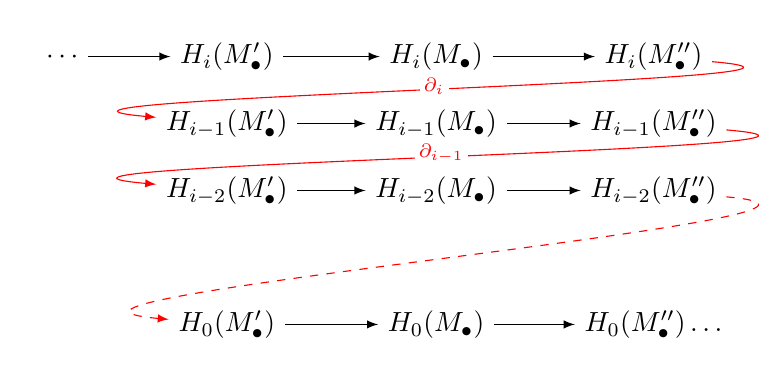
\begin{tikzpicture}[descr/.style={fill=white,inner sep=1.5pt}]
        \matrix (m) [
            matrix of math nodes,
            row sep=1em,
            column sep=2.5em,
            text height=1.5ex, text depth=0.25ex
        ]
        { \cdots & H_i(M'_\bullet) & H_i(M_\bullet) & H_i(M''_\bullet) \\
            & H_{i-1}(M'_\bullet) & H_{i-1}(M_\bullet) & H_{i-1}(M''_\bullet) \\
            & H_{i-2}(M'_\bullet) & H_{i-2}(M_\bullet) & H_{i-2}(M''_\bullet) \\
            & \mbox{}         &                 & \mbox{}         \\
            & H_0(M'_\bullet) & H_0(M_\bullet) & H_0(M''_\bullet) \ldots \\
        };

        \path[overlay,->, font=\scriptsize,>=latex]
        (m-1-1) edge (m-1-2)
        (m-1-2) edge (m-1-3)
        (m-1-3) edge (m-1-4)
        (m-1-4) edge[out=355,in=175,red] node[descr,yshift=0.3ex] {$\partial_i$} (m-2-2)
        (m-2-2) edge (m-2-3)
        (m-2-3) edge (m-2-4)
        (m-2-4) edge[out=355,in=175,red] node[descr,yshift=0.3ex] {$\partial_{i-1}$} (m-3-2)
        (m-3-2) edge (m-3-3)
        (m-3-3) edge (m-3-4)
        (m-3-4) edge[out=355,in=175,dashed,red] (m-5-2)
        (m-5-2) edge (m-5-3)
        (m-5-3) edge (m-5-4);
\end{tikzpicture}
    
      where the map $\color{red}{\partial_i}$ is defined as follows: 
      
      Given $z \in \ker(d_i: M''_i \to M''_{i-1})$,
 since $p$ is onto,     we may find a $w \in M_i$ such that $p_i(w) = z$. For any choice of such a $w$, we have
 $p(d(w)) = d(p(w)) = d(z) = 0$ and hence, by the exactness in the middle of the original s.e.s.,
 there is a unique $u \in M'_{i-1}$ such that $j(u) = d(w)$.
      We have $j d(u) = d(j(u)) = d(d(w)) = 0$ and thus, since $j$ is one-to-one, $u \in \ker(d_{i-1})$. 
      We set $\partial_i(\overline{z}) = \overline{u} \in H_{i-1}(M'_\cdot)$.
\end{thm}
\begin{proof}
%One needs to show that the connecting maps $\partial_i$ are well defined with respect to changing the choice of $w$ and that the given long sequence is indeed exact. Both of these tasks involve diagram chases much like in the proof of the Sanke Lemma. I will leave it to the diligent readers to chase the appropriate diagrams.

The theorem follows from several applications of the Snake Lemma:
\begin{itemize}
\item First we note that for any $n$, we have  a commutative diagram
\[ \xymatrix{ 0 \ar[r] & M'_n \ar[r]\ar[d]^{d_n^{M'}} & M_n \ar[r]\ar[d]^{d_n^{M}}& M''_n \ar[r]\ar[d]^{d_n^{M''}}  & 0
\\  0 \ar[r] & M'_{n-1} \ar[r] & M_{n-1} \ar[r] & M''_{n-1} \ar[r] & 0, } \]
so by the Snake Lemma we get exact sequences
\[0\to Z_n(M'_\bullet)\to  Z_n(M_\bullet) \to  Z_n(M''_\bullet)\]
\[M'_n/B_n (M'_\bullet) \to M_n/B_n (M_\bullet) \to M''_n/B_n (M''_\bullet) \to 0 .\]
\item Next we observe that since the boundaries $B_n$ are contained in the kernel of the differential $d_{n}$ and since the image of $d_{n}$ is contained in $Z_n$, the universal mapping property of the quotient gives that the differentials $d_n$ for the three complexes induce vertical maps as follows
\[
\xymatrix{
& M'_n/B_n (M'_\bullet) \ar[r] \ar[d]^{\ov{d}_n^{M'}} &M_n/B_n (M_\bullet) \ar[r] \ar[d]^{\ov{d}_n^{M}} &M''_n/B_n (M''_\bullet) \ar[r] \ar[d]^{\ov{d}_n^{M''}} &0\\
0\ar[r] & Z_{n-1}(M'_\bullet)\ar[r] &  Z_{n-1}(M_\bullet) \ar[r]&  Z_{n-1}(M''_\bullet) 
}
\]
\item observe that the kernel of $\ov{d}_n$ is $H_n$ and the cokernel of $\ov{d}_n$ is $H_{n-1}$ therefore the Snake Lemma applied to the diagram in the previous bullet point yields a six term exact sequence
\[
H_n(M'_\bullet) \to H_n(M_\bullet) \to H_n(M''_\bullet) \xra{\partial} H_{n-1}(M'_\bullet) \to H_{n-1}(M_\bullet) \to H_{n-1}(M''_\bullet)
\]
Comparing the description of $\partial$ given by the Snake Lemma and the description of $\partial_n$ above one sees that these maps are the same.\qedhere
\end{itemize}
\end{proof}

\begin{comment}
\begin{ex}
The long exact sequence in homology is used in topology to compute the homology groups of quotient spaces. Let $X$ be the simplicial complex of Example \ref{ex:simplicialhomology} and let $A$ be the subset formed by the three vertices. Then there is an obvious inclusion $A\subseteq X$, which leads to an inclusion of chain complexes $C_\bullet(A)\hookrightarrow C_\bullet(X)$. Ler $D_\bullet$ be the cokernel of this inclusion, leading to a s.e.s of chain complexes
\[
0\to C_\bullet(A)\xra{i} C_\bullet(X) \xra{\pi} D_\bullet \to 0.
\]
We could compute $D_\bullet$ explicitly and find its homology. Instead, let's compute the homology of $D_\bullet$ by using nothing but the l.e.s. in homology: for $i<0$ or $i\geq 2$ we have s.e.s
\[
0=H_i(X) \to H_i(D_\bullet)\to  H_{i-1}(A)=0
\]
which yield $H_i( D_\bullet)=0$ for $i\geq 2$ and $i<0$. Now for the more interesting portion of the l.e.s:
\[
0=H_1(A) \to H_1(X) \to H_1( D_\bullet) \to H_0(A)\xra{H_0(i)} H_0(X) \to H_0( D_\bullet)\to 0.
\]
Substituting the known homology groups for $X, A$ (see Example \ref{ex:homologygps}) we have:
\[
0\to \Z \to H_1( D_\bullet) \xra{\partial_1} \Z^3\xra{H_0(i)=\begin{bmatrix} 1 & 1 & 1\end{bmatrix}} \Z \to H_0( D_\bullet)\to 0.
\]
Since the map $H_0(i)$ is surjective, we deduce $H_0(D_\bullet) =0$. Also the kernel of this map is 
$K=\Z(\{1\}-\{2\})\oplus \Z(\{1\}-\{3\})\cong \Z^2$. By the exactness of the above l.e.s, $K=\im(\partial_1)$, so we can write a s.e.s.
\[
0\to \Z\to  H_1( D_\bullet) \xra{\partial_1} K\cong\Z^2\to 0.
\]
Finally, since $\Z^2$ is free, hence projective, the s.e.s above splits and yields $ H_1( D_\bullet)\cong \Z\oplus \Z^2\cong \Z^3$.

The importance of this computation to topology is that it recovers the (reduced) homology groups of the quotient space $X/A$. This is defined as the space obtained from $X$ by collapsing all the points of $A$ to a single point. In our example this results in $X/A$ being a bouquet of 3 circles. 

Then the reduced homology groups of $X/A$ (also called the relative homology groups of $X$ with respect to $A$) are given by $\widetilde{H_i}(X/A)=H_i(X,A)=H_i(D_\bullet)=\begin{cases} \Z^3& i=1, \\ 0 &\text{ otherwise}.\end{cases}$
Finally, the reduced homology groups relate to the ordinary  homology groups by 
$\widetilde{H_i}(X/A)=\begin{cases}H_0(X/A)/\Z& i=0, \\ H_i(X/A) &\text{ otherwise}\end{cases}$, hence we deduce
\[
H_i(X/A)=\begin{cases}\Z & i=0, \\ \Z^3& i=1, \\ 0 &\text{ otherwise}.\end{cases}
\]


\end{ex}
\end{comment}

\begin{cor}[Two out of three exactness]
 If $0 \to M'_\bullet \to M_\bullet \to M''_\bullet\to 0$ is a short exact sequence of chain complexes of left $R$-modules and if any two of the three complexes are exact, then the third complex is also exact.
\end{cor}
\begin{proof}
Recall that a complex is exact if and only if all its homology modules are equal to 0. Now if two of the three given complexes are exact (say $M_\bullet$ and $M''_\bullet$ are exact for concreteness), it means that in the long exact sequence in homology we have two zeros surrounding each of the homology modules of the third complex ($M'_\bullet$) as follows:
$$
      \cdots  \xra{H_i(p)} 0 \xra{\partial_i}
      H_{i-1}(M'_\bullet) \xra{H_{i-1}(j)} 0 \xra{H_{i-1}(p)} \cdots
      $$
      The presence of the 0 homology modules implies that $\partial_i=0=H_{i-1}(p)$, and the exactness yields $H_{i-1}(M'_\bullet)=\ker(H_{i-1}(j))=\im(\partial_i)=0$ for any $i\in \Z$. Thus $M'_\bullet$ is exact.
\end{proof}

\subsection{Homotopy of chain maps}

  \begin{defn} Suppose $M_\bullet$ and $N_\bullet$ are two chain complexes of $R$-modules and $f,g: M_\bullet \to N_\bullet$ are two chain maps joining them.
    We say $f$ and $g$ are 
{\em homotopic} (or sometimes {\em chain homotopic}), written $f \htpy g$,  if there is a family of $R$-maps $h_i: M_i \to N_{i+1}$, $i \in \Z$, such that
$$
d^N_{i+1} \circ h_i + h_{i-1} \circ d^M_i = f_i - g_i
$$
for all $i$. (Succinctly, $dh + hd = f -g$.) Such a  family of maps $\{h_i\}_{i \in \Z}$ is called a {\em chain homotopy} joining $f$ to $g$.
A chain map is called {\em null-homotopic} if $f \htpy 0$. 
 \end{defn}

 Here is a picture of a chain homotopy
 $$
 \xymatrix{
   \cdots \ar[r] & M_{i+1} \ar[r] \ar[d] \ar[ld] & M_{i} \ar[r] \ar[d]^{{\tiny f_i-g_i}} \ar[ld]^{{\tiny h_i}} & M_{i-1} \ar[r] \ar[d] \ar[ld] & \cdots \ar[ld] \\
 \cdots \ar[r] & N_{i+1} \ar[r] &N_{i} \ar[r] &N_{i-1} \ar[r] & \cdots. \\
}
$$
 The squares commute but the triangles do not. Rather, the sum of the two compositions in each rhombus
 $$
\xymatrix{
  &  \bullet \ar[dl] \ar[r] & \bullet \ar[ld] \\
  \bullet \ar[r] & \bullet \\
}
$$
occuring in this diagram is equal to the difference of $f$ and $g$. 

 
\begin{ex} If $f,g: X \to Y$ are continuous maps between topoogical spaces that are homotopic in the sense of topology, 
then the induced maps on singular chain complexes $f_*, g_*: C_\bullet(X) \to C_\bullet(Y)$ are chain homotopic.
\end{ex}


 \begin{ex} I claim the chain map pictured below is null homotopic:
   $$
   \xymatrix{
     \cdots \ar[r] & 0 \ar[r]\ar[d] &  0 \ar[d] \ar[r] &  \Z \ar[r] \ar[d]^{17} & 0 \ar[r] \ar[d]& \cdots \\
     \cdots \ar[r] & 0 \ar[r] & \Z \ar[r]^{17} &  \Z \ar[r] & 0 \ar[r] & \cdots \\
   }
   $$
   A null-homotopy is given by the diagram
   $$
   \xymatrix{
     \cdots \ar[r] &  0 \ar[d] \ar[r] \ar[dl] &  \Z \ar[r] \ar[d]^{17} \ar[dl]_1 & 0 \ar[r] \ar[d] \ar[dl] & \cdots \\
     \cdots \ar[r] &  \Z \ar[r]^{17} &  \Z \ar[r] & 0 \ar[r] & \cdots \\
   }
   $$
  \end{ex}
   
%  \begin{lem} The relation chain homotopy is an equivalence relation on the set of all chain maps between two complexes.
%
%Moreover,  it is preserved under composition and it respects addition and subtraction
%    in the following senses: if $f,g: M_\bullet \to N_\bullet$ are chain maps and $f \htpy g$, then 
%\begin{itemize}
%\item $f \circ \be \htpy g \circ \be$ for all chain maps $\be: L_\cdot \to M_\bullet$,
%\item  $\a \circ f \htpy \a \circ g$ for all chain maps $\a: N_\bullet \to T_\cdot$, and
%\item $f  +  f' \htpy g + g'$ and $f  -  f' \htpy g - g'$ whenever
%$f', g': M_\bullet \to N_\bullet$ are chain maps such that $f' \htpy g'$. 
%\end{itemize}
%
%
%     In particular, two chain maps are homotopic if and only if their difference is null-homotopic.
%   \end{lem}
%   
%
%\begin{rem} Another way of phrasing the Lemma is that in the additive category $\Cat{$R$-complexes}$, the collection of null-homotopic maps forms
%the analogue of a two-sided ideal for additive categories.  It does indeed make sense to mod out by the set of null-homotopic maps, and one gets
%a category known as the {\em homotopy category} of complexes of $R$-modules. I might say more about this later. 
%\end{rem} 
%
%
%\begin{proof} I'll leave it to you to prove it is an equivalence relation. 
%
%
%Say $h$ is a homotopy joining $f$ to $g$; i.e., for all $i$
%  $$
%  d^N_{i+1} \circ h_i + h_{i-1} \circ d^M_i = f_i - g_i.
%  $$
%  Apply $\a \circ -$ or $- \circ \be$ to this equation to deduce that $\a \circ h$ and $h \circ \be$ are homotopies joining
%  $\a \circ f$ to $\a \circ g$ and $f \circ \be$ to $g \circ \be$. For example,  applying $\a$ gives
%$$
%\a  (dh + hd) = \a(f - g) \Rightarrow
%\a dh + \a hd = \a f  - \a g \Rightarrow
%d (\a h) + (\a h) d = \a f - \a g
%$$
%where the second equality using that $\a$ is a chain map. 
%
%  Say $h'$ is a homotopy joining $f'$ to $g'$, so that for all $i$ we have
%  $$
%  d^N_{i+1} \circ h'_i + h'_{i-1} \circ d^M_i = f'_i - g'_i.
%  $$
%  Now just add or subtract this equation from the previous one for each $i$ to show that $h + h'$ and $h - h'$
%  are homotopies joining $f + f'$ to $g + g'$ and $f - f'$ to $g - g'$. 
%\end{proof}
%
%
  
  
 The main point of chain homotopy is given by the following result:

 \begin{prop}
 \label{prop:homotopy}
  Homotopic chain maps induce the same map on homology: If $f$ and $g$ are chain maps from $(M_\bullet, d^M)$ to $(N_\bullet, d^N)$ and they are homotopic,
   then $H_i(f) = H_i(g)$ for all $i$. 
   
   In particular, a null homotopic map induces the $0$ map on homology. 
 \end{prop}

 \begin{proof} We prove the second assertion first. Suppose $f$ is null-homotopic. For any $i$,
   let  $\ov{z} \in H_i(M)$ be a class represented by an element $z \in \ker(d_i: M_i \to M_{i-1})$.
   Since $f$ is null-homotopic, there is a $h$ such that  $d^N h + h d^M = f$.
   So $f(z) = d^N(h(z)) + h(d^M(z)) = d^N(h(z))$ since $d(z) = 0$. This gives $f(z) \in \im(d)$ and hence $\ov{f(z)} = 0$ in $H_i(N_\bullet)$.

If $f \htpy g$, then $f- g$ is null-homotopic, so that $H_i(f-g) = 0$, by what we just proved. Since $H_i$ is additive, 
  we have $0 = H_i(f-g) = H_i(f) - H_i(g)$. 
   \end{proof}

   \begin{ex} The converse of this proposition is false. For example, the chain map of $\Z$-modules pictured as
   $$
   \xymatrix{
     \cdots \ar[r] & 0 \ar[r]\ar[d] &   0 \ar[d] \ar[r] &   \Z/2\Z \ar[r] \ar[d]^{2} & 0 \ar[r] \ar[d]& \cdots \\
     \cdots \ar[r] & 0 \ar[r] &   \Z/4\Z \ar[r]^{2} &  \Z/4\Z \ar[r] & 0 \ar[r] & \cdots \\
   }
   $$
   induces the $0$ map on all homology groups, but it  is not null homotopic. Indeed, the only possible homotopy would
   be $0$ in all degrees except one, in which it would be a map $h_0: \langle \Z/2\Z  \rangle \to \Z/4\Z$. The only possibilities for $h_0$
   are the $0$ map and the map of multiplication by 2, but neither works.
 \end{ex}
 


\Nov{22}
 
 \ssec{Projective and Injective Resolutions}


\sssec{Free and Projective resolutions}

\begin{defn} Let $M$ be an $R$-module. A \DEF{free resolution} of $M$ is a chain complex $F_\bullet$ of free $R$-modules 
\[ \cdots F_3 \xra{d_3} F_2 \xra{d_2} F_1 \xra{d_1} F_0 \to 0 \cdots \]
along with a map $\pi: F_0\to M$ such that the augmented complex
\[ \cdots F_3 \xra{d_3} F_2 \xra{d_2} F_1 \xra{d_1} F_0 \xra{\pi} M \to 0 \cdots \]
is exact.
Similarly, a \DEF{projective resolution} is a complex of projective modules that satisfies the same conditions.\end{defn}

In particular, a free or projective resolution of $M$ is a chain complex such that $H_i(P_\bullet) = 0$ for $i\neq 0$ and $H_0(P_\bullet) \cong M$.


Free resolutions always exist:

\begin{lem} Every $R$-module admits a free resolution.
\end{lem}
\begin{proof}
Let $M$ be an $R$-module. There is a surjection $\pi$ from a free module $F_0$ onto $M$ (given by mapping a free basis of a free module to a generating set for $M$). Then, $\ker(\pi)\subseteq F_0$ is a module, and there is a surjection $\pi_1$ from a free module $F_1$ onto $\ker(\pi)$; let $d_1:F_1 \to F_0$ be the composition of $\pi_1$ and the inclusion map. Take a surjection from a free module onto $\ker(d_1)$, and continue like so.
\end{proof}

A free or projective resolution can be thought of as an approximation of $M$ by free/projective modules via a sort of inclusion/exclusion method: A crude approximation of $M$ is a free module $F_0$ that surjects onto it. Such an approximation is too big, so we want to subtract the kernel of $\pi$, and we take a free module that surjects onto the kernel for $F_1 \xra{d_1} F_0$. But we might consider this as subtracting too much, since $F_1$ may properly surject onto, so be bigger than, the kernel. And so on.


They need not be unique.

\begin{ex} For a ring $R$, a free resolution of the free module $R$ is $0 \to R \to 0$, with the map $\pi:R\xra{1} R$. We could also take $0 \to R \xra{\begin{bmatrix} 1 \\ -1\end{bmatrix}} R^2 \to 0$, with the map $\pi: R^2 \xra{ \begin{bmatrix} 1 & 1\end{bmatrix} } R$.
\end{ex}


\begin{ex} Let $K$ be a field, and $R=K[x,y]$ be a polynomial ring over $K$. Take $M=R/(x,y)$. There is a surjection $\pi:R\to M$. The kernel of $\pi$ is generated by $x$ and $y$, so we can take $d_1:R^2 \xra{\begin{bmatrix} x & y\end{bmatrix}} R$. We need to find the kernel of $d_1$: if $xf+yg=0$ in $R$, then $xf=-yg$, and since $R$ is a UFD, we have $f=yh, g=-xh$ for some $h\in R$. Thus, $\ker(d_1) = R\cdot \begin{bmatrix} y \\ -x\end{bmatrix}$, so we can take
\[ 0 \to R \xra{\begin{bmatrix} y \\ -x\end{bmatrix}} R^2 \xra{\begin{bmatrix} x & y\end{bmatrix}} R \to 0\]
as a free resolution.
\end{ex}

\begin{ex} Let $K$ be a field, and $R=K[x,y]/(xy)$. Take $M=R/(x)$. There is a surjection $\pi:R\to M$. The kernel of this is generated by $(x)$, so we can take $d_1: R \xra{x} R$. The kernel of this consists of the elements killed by $x$ in $R$, which is $(y)$, so we can take $d_2: \xra{y} R$. It's now clear this keeps repeating:
\[ \cdots \to R \xra{x} R \xra{y} R \xra{x} R \xra{y} R  \xra{x} R \to 0. \]
\end{ex}

\sssec{Injective resolutions}

\begin{defn} For a ring $R$ and $R$-module $M$, an \DEF{injective resolution} of $M$ is complex of the form
$$
\cdots \to 0 \to E^0 \xra{d^0} E^1 \xra{d^1}  E^2 \xra{d^2}  \cdots,
$$
(with $E^0$ in homological degree zero) such that each $E^i$ is injective for all $i$, 
together with an $R$-map $M \xra{i} E^0$ such that the augmented sequence
$$
0 \to M \xra{i} E^0 \xra{d^0} E^1 \xra{d^1}  E^2 \xra{d^2}  \cdots
$$
is an exact complex.
\end{defn}

\begin{rem} The notation above follows \DEF{cohmological indexing}, in which we write a complex \[ \cdots \to M_2 \xra{d_2} M_1 \xra{d_1}  M_0 \xra{d_0}  M_{-1} \xra{d_{-1}} M_{-2} \to\cdots\] 
as 
\[ \cdots \to N^{-2} \xra{d^{-2}} N^{-1} \xra{d_{-1}} N^0 \xra{d^0}  N^{1} \xra{d^1} N^{2} \to\cdots,\]
where $N^i = M_{-i}$ and $d^{i}=d_{-i}$.
\end{rem} 

\Nov{29}

Injective resolutions also exist.

\begin{prop} Every $R$-module admits an injective resolution.
\end{prop}

\begin{proof} Given a module $M$, by a result above we can find an injective $R$-linear map $j: M \to E^0$ with $E^0$ injective. 
Let $N = \coker(j) = E^0/\im(j)$ and apply this result again to obtain a injective $R$-module map $N \to E^1$ with $E^1$ injective. 
Let $E^0 \to E^1$ be the composition of $E^0 \to N \to E^1$. Then we have a l.e.s $0 \to N \to E^1 \to E^2$.
Repeating this process (by taking the cokernel of $E^1 \to E^2$ and injecting it into an injective $R$-module, etc.), we build a (possibly never-ending)
injective resolution of $M$.
\end{proof}


\begin{ex} Let us  find an injective resolution of $\Z$ as a module over itself. We have the evident embedding $\Z \to \Q$ and we know $\Q$ is injective since
  it is divisible. The cokernel is $\Q/\Z$, which is injective since it too is divisible. Thus
$$
0 \to \Z \to \Q \to \Q/\Z \to 0 \to \cdots
$$
is an injective resolution of $\Z$.
\end{ex}


\begin{ex} 
Let's find an injective resolution of $\Z/n\Z$ as a $\Z$-module. We have
$$
0 \to \Z/n\Z \to \Q/\Z \to E^1 \to 0 \to \cdots
$$
where $E^1$ is the quotient of $\Q/\Z$ by the subgroup generated by $1/n + \Z$. In other words
$E^1 = \frac{\Q}{\Z + \Z \cdot \frac{1}{n}}$. Then $E^1$ is divisible and hence injective. 
\end{ex}

\begin{defn} Let $M$ and $N$ be $R$-modules, and $P_\bullet$ and $Q_\bullet$ be two complexes such that $P_i=0$ and $Q_i=0$ for all $i<0$. Suppose we have maps $P_0 \xra{p} M$ and $Q_0 \xra{q} N$. We say that a chain map $\tilde{f}:P_\bullet \to Q_\bullet$ \DEF{lifts} an $R$-module map $f:M\to N$ if the diagram of complexes
\[ \xymatrix{ P_\bullet \ar[r]^{\tilde{f}} \ar[d]_p & Q_\bullet \ar[d]^q  \\ M \ar[r]^f & N}\] commutes. Equivalently, such a map is a lift if the diagram
\[ \xymatrix{ \cdots \ar[r] & P_2 \ar[d]^{\tilde{f}_2} \ar[r] & P_1 \ar[d]^{\tilde{f}_1}\ar[r] & P_0 \ar[d]^{\tilde{f}_0} \ar[r]^p & M \ar[r] \ar[d]^{f} & 0 \ar[r] & \cdots \\
\cdots \ar[r] & Q_2 \ar[r] & Q_1 \ar[r] & Q_0 \ar[r]^q & M \ar[r] & 0 \ar[r] & \cdots}\]
commutes.

Similarly, in cohomological notation, if $P^\bullet$ and $Q^\bullet$ be two complexes such that $P^i=0$ and $Q^i=0$ for all $i<0$ and  we have maps $M \xra{p} P^0$ and $N \xra{q} Q^0$, we say that a chain map $\tilde{f}:P^\bullet \to Q^\bullet$ \DEF{lifts} an $R$-module map $f:M\to N$ if the diagram of complexes
\[ \xymatrix{ P^\bullet \ar[r]^{\tilde{f}}  & Q^\bullet   \\ M \ar[r]^f \ar[u]^p & N \ar[u]_q}\] commutes.
\end{defn}


\begin{thm} \label{thm121b} Let $M$ and $N$ be $R$-modules, $f: M \to N$ an $R$-module homomorphism. 
Consider two complexes
\[
P_\bullet=  \qquad  \cdots \to P_2 \to P_1\to P_0 \to 0 \to 0 \to \cdots
\]
\[
Q_\bullet = \qquad \cdots \to Q_2 \to Q_1\to Q_0 \to 0 \to 0 \to \cdots
\]
with maps $P_0 \xra{p} M$ and $Q_0 \xra{q} N$.
Suppose that $P_i$ is projective for all $i$ and that the augmentation of $Q_\bullet$,
\[
\qquad \cdots \to Q_2 \to Q_1\to Q_0 \xra{q} N \to 0 \to \cdots,
\]
is exact.
  
    Then there is a lift $\tilde{f}: P_\bullet \to Q_\bullet$ of $f$. Moreover, $\tilde{f}$ is unique up to homotopy: if $\tilde{f}': P_\bullet \to Q_\bullet$ is another lift of $f$, then $\tilde{f} \htpy \tilde{f}'$. 
\end{thm}

\def\tf{\tilde{f}}

\begin{proof} For existence, as illustrated below,
\[\xymatrix@R=4em@C=4em{ \cdots \ar[r] & P_2 \ar[r]^{d^P_2} \ar@{-->}[d]^{\tilde{f}_2} &  P_1 \ar[r]^{d^P_1} \ar@{-->}[d]^{\tilde{f}_1}  & P_0 \ar[r]^{p} \ar@{-->}[d]^{\tilde{f}_0} & M \ar[r] \ar[d]^{f} & 0 \\ 
\cdots \ar[r] & Q_2 \ar[r]^{d^Q_2} &  Q_1 \ar[r]^{d^Q_1} & Q_0 \ar[r]^{q} & N \ar[r] & 0, }\]
we need to construct maps $\tf_i: P_i \to Q_i$ for $i   \geq 0$ such that $q \tf_0 = f  p$
and $d^Q_i  \tf_i = \tf_{i-1}  d^P_i$ for $i \geq 1$. To construct $\tf_0$, we merely use the definition of projective and the diagram
$$
\xymatrix{
& P_0 \ar[d]^{f  p}   \ar@{-->}[dl]_{\exists \tf_0} \\
Q_0 \ar[r]^q & N \ar[r] & 0. \\
}
$$
Suppose we have constructed maps $\tf_0, \dots, \tf_n$ for some $n \geq 0$  so that
 $d^Q_i  \tf_i = \tf_{i-1} d^P_i$ for $1 \leq i \leq n$. (When $n = 0$, the condition is vacuous.) Then $d_n^Q \tf_n d_{n+1}^P = \tf_{n-1} d_n^P d_{n+1}^P = 0$, so $\im(\tf_n d_{n+1}^P )\subseteq Z_{n}(Q_\bullet)=B_{n}(Q_\bullet)$, using exactness of $Q_\bullet$.  Use the definition of projective again with the diagram
$$
\xymatrix{
& P_{n+1} \ar[d]^{\tf_n  d^P_{n+1}}   \ar@{-->}[dl]_{\exists \tf_{n+1}} \\
Q_{n+1} \ar[r]^{d^Q_{n+1}} & B_{n}(Q_\bullet) \ar[r] & 0 
}
$$
 to construct $\tf_{n+1}$ such that  $d^Q_{n+1} \tf_{n+1} = \tf_{n}  d^P_n$ holds too.  This proves existence. 

\Dec{1}


For uniqueness, suppose $\tilde{f}'$ is another such chain map.  Observe that $\tilde{f} - \tilde{f}'$ is a chain map from $P_\bullet \to Q_\bullet$ that extends the zero map from $M$
to $N$. Thus, it suffices to prove that if $\tf: P_\bullet \to Q_\bullet$ is a lift of the zero map, then $\tf$ is null-homotopic. That is, 
\[\xymatrix@R=4em@C=4em{ \cdots \ar[r] & P_2 \ar[r]^{d^P_2} \ar[d]^{\tilde{f}_2} &  P_1 \ar[r]^{d^P_1} \ar[d]^{\tilde{f}_1} \ar@{-->}[dl]_{h_1} & P_0 \ar[r]^{p} \ar[d]^{\tilde{f}_0} \ar@{-->}[dl]_{h_0} & M \ar[r] \ar[d]^{0} & 0 \\ 
\cdots \ar[r] & Q_2 \ar[r]^{d^Q_2} &  Q_1 \ar[r]^{d^Q_1} & Q_0 \ar[r]^{q} & N \ar[r] & 0, }\]
we need to show there are maps
$h_i: P_i \to Q_{i+1}$ for $i \geq 0$ such that $d^Q_{i+1}  h_i + h_{i-1}  d^P_i = \tf_i$ for all $i \geq 0$. (In the latter equation,
when $i = 0$ we have $h_{-1} = 0$.)

Since $q \circ \tf_0 = 0 p = 0$, the image of $\tf_0$ is contained in $\ker(q) = \im(d^Q_1)=B_0(Q_\bullet)$ and so since $P_0$ is projective, considering the diagram
$$
\xymatrix{
& P_0 \ar[d]^{\tf_0}   \ar@{-->}[dl]_{\exists h_0} \\
Q_1 \ar[r]^{d_1^Q} & B_0(Q_\bullet) \ar[r] & 0. \\
}
$$ there is a map $h_0: P_0 \to Q_1$ such 
that $d_1^Q \circ h_0 = g_0$ as needed. 

We will proceed inductively again. When we separate out the ``new part'' in the null-homotopy equation, we get $d^Q_{n+1} h_n = \tf_n - h_{n-1}  d^P_n$, so we want to use the projective lifting property to the map on the right; to do that, it should be in the image of the differential through which we want to lift it. Hence, we will be interested in showing that the image such a map consists of boundaries.

So, as part of the base case of our induction, we observe that
\[ d_1^Q(\tf_1 - h_0 d_1^P) = d_1^Q \tf_1 - d_1^Q h_0 d_1^P = \tf_0 d_1^P - d_1^Q h_0 d_1^P = d_1^Q h_0 d_1^P - d_1^Q h_0 d_1^P = 0,\]
so $\im(\tf_1 - h_0 d_1^P) \subseteq Z_1(Q_\bullet) = B_1(Q_\bullet)$.

Suppose maps $h_0, \dots, h_n$ have been constructed for some $n \geq 0$ with $ d^Q_{n+1} h_n + h_{n-1}  d^P_n=\tf_n $, and that $\im(\tf_{n+1} - h_n d^P_{n+1}) \subseteq B_{n+1}(Q_\bullet)$. 

Since $P_{n+1}$ is projective, considering the diagram
$$
\xymatrix{
& P_{n+1} \ar[d]^{\tf_{n+1}-h_n d^P_{n+1}}   \ar@{-->}[dl]_{\exists h_{n+1}} \\
Q_{n+2} \ar[r]^{d^Q_{n+2}} & B_{n+1}(Q_\bullet) \ar[r] & 0, \\
}
$$ there is a map $h_{n+1}: P_{n+1} \to Q_{n+2}$ such 
that $d_{n+2}^Q \circ h_{n+1} = \tf_{n+1}-h_n d^P_{n+1}$. Then
\[ d^Q_{n+2}(\tf_{n+2} - h_{n+1} d^P_{n+2}) = \tf_{n+1} d^P_{n+2} - d^Q_{n+2} h_{n+1} d^P_{n+2} = (\tf_{n+1} - d^Q_{n+2} h_{n+1}) d^P_{n+2} = h_n d^P_{n+1} d^P_{n+2} = 0.\]
Again using exactness of $Q_\bullet$, we see that $\im(\tf_{n+2} - h_{n+1} d^P_{n+2}) \subseteq B_{n+2}(Q_\bullet)$. Thus, by induction, we can construct such a map $h$.
\end{proof}

\begin{defn} Given two chain complexes $(M_\bullet, d)$ and $(N_\bullet, d)$, a chain map $f: M_\bullet \to N_\bullet$ is called a \DEF{homotopy equivalence}, written $f: M_\bullet \xra{\simeq}
  N_\bullet$, if there is a chain map $g: N_\bullet \to M_\bullet$ such 
that both compositions are homotopic to the identity map: $f \circ g \htpy \id_N$ and $g \circ f \htpy \id_M$. 
\end{defn}

\begin{rem}
If $f: M_\bullet \to N_\bullet$ is  a homotopy equivalence, then $f$ is a quasi-isomorphism. Indeed, using Proposition \ref{prop:homotopy} we see that  $H_i(f)\circ H_i(g)=H_i(f\circ g)=H_i(\id_N)=\id_{H_i(M_\bullet)}$ and $H_i(g)\circ H_i(f)=H_i(g\circ f)=H_i(\id_M)=\id_{H_i(N_\bullet)}$.
\end{rem}



\begin{ex} Let $M$ be an $R$-module and let
$$
\cdots \to P_2 \to P_1 \to P_0 \to 0 \to \cdots
$$
along with $\pi: P_0 \onto M$ form a projective resolution of $M$.  We may interpret this as an example of a quasi-isomorphism:
The map $\pi$ induces a chain map
$$
\pi: P_\bullet \to M[0]
$$
which is the map $\pi$ in degree $0$ and (necessarily) the zero map in all other degrees.
(By abuse of notation, we call the chain map $\pi$ too.) Here is a picture of the chain map $\pi$:
$$
\xymatrix{
  \cdots \ar[r] &  P_2 \ar[r] \ar[d] & P_1 \ar[r] \ar[d] & P_0 \ar[r] \ar[d] & 0 \ar[r] \ar[d] & \cdots \\
  \cdots \ar[r] &  0  \ar[r] & 0 \ar[r]& M \ar[r] & 0 \ar[r] & \cdots. \\
}
$$
On homology we have $H_i(P_\bullet) = 0$ for all $i \ne 0$ and $H_i(M[0]) = 0$ for all $i \ne 0$, so that $H_i(\pi)$ is an isomorphism, vacuouly, for all $i \ne 0$. 
In degree $0$, the map
$$
H_0(\pi): H_0(P_\bullet) \to H_0(M)
$$
is the isomorphism $\overline{\pi}: \coker(d_0)  = P_0/\im(d_0) = P_0/\ker(\pi)  \xra{\cong} M$ induced by $\pi$. So $\pi$ is indeed a quasi-isomorphism.

However, I clam that $\pi$ is not a homotopy equivalence in general. If it were, there would be a chain map $g: M \to P_\bullet$ such that $\pi \circ g \htpy \id_M$ (and also for the other composition).
Note that the chain map $g$ is really just a map $g_0: M \to P_0$. Let $h$ be a homotopy realizing $\pi \circ g \htpy \id_M$. 
Since $M = M[0]$ is only nonzero in degree $0$, $h$ has to be the zero map. It follows that $\pi \circ g = \id_M$ and hence
the composition
$$
M \xra{g_0} P_0 \xra{\pi} M 
$$
is the identity. That is, $M$ is isomorphic to a summand of $P_0$ and hence $M$ itself is projective. But, of course $M$ is an arbitrary module so it need not be projective.
\end{ex}


\begin{cor} \label{cor122}
  Any two projective resolutions of the same module are homotopy equivalent: if $p: C_\bullet \xra{\sim} M$ and
$q: Q_\bullet \xra{\sim} M$ are two projective resolutions of a module $M$, then there is a homotopy equivalence $g: P_\bullet \xra{\simeq} Q_\bullet$
such that the triangle diagram of chain complexes
$$
\xymatrix{
P_\bullet \ar[rd]^p_\sim \ar[dd]^g_\simeq \\
& M \\
Q_\bullet \ar[ru]_q^\sim \\
}
$$
commutes. (Equvialently, $g$ is a lift of the identity map on $M$.) Moreover, $g$ is unique up to homotopy.
\end{cor}



\begin{proof} Applying the previous result to the identity
  map on $M$ gives a chain map $g: P_\bullet \to Q_\bullet$ such that $q \circ g = p$. Moreover, $g$ is unique up to homotopy by
the uniqueness clause of the previous result. 

By interchanging the roles of $P_\bullet$ and $Q_\bullet$ we get a chain map
$f: Q_\bullet \to P_\bullet$ such that $p \circ f = q$. The composition $f \circ g$ is a chain endomorphism of $P_\bullet$ such that $p \circ f \circ g =
p$. Since we also have $p \circ id_{P_\bullet} = p$, 
the uniqueness clause of the previous result gives that $f \circ g$ is homotopic to $\id_{C_\bullet}$. Similarly, 
$g \circ f$ is homotopic to $\id_{Q_\bullet}$. 
\end{proof}


I'll skip the proof of the following two statements. Both the statements and the proofs are given by flipping the orientation of all the arrows involved in the
previous two statements and proofs.

\begin{thm} \label{thm121c}
  Let $M$ and $N$ be $R$-modules, $f: M \to N$ an $R$-module homomorphism, and $i: M \xra{\sim} E^\bullet$ and $j: N \xra{\sim} F^\bullet$ injective resolutions. Then there is
a lift $\tilde{f}:E^\bullet \to F^\bullet$ of $f$, and such a lift is unique up to homotopy.
\end{thm}

\begin{cor} Any two injective resolutions of the same module are homotopy equivalent via a chain map that is unique up to homotopy. 
\end{cor}

\begin{exer} If $g$ is a homotopy equivalence, and $F$ is an additive covariant functor, then $F(g)$ is a homotopy equivalence.
\end{exer}


\ssec{Derived functors}


\begin{defn}
\label{def:leftderived}
 Let $R$ and $S$ be rings and $F: \Mod{R} \to \Mod{S}$ be a right exact covariant functor. 
For each $j \geq 0$, we define a functor $\bL_j F : \Mod{R} \to \Mod{S}$ as follows:

For every $R$-module fix a projective resolution $P_\bullet^M \xra{p_M} M$, and for every $R$-module homomorphism $f: M \to N$, fix a chain map $\tilde{f}: P_\bullet^M \to P_\bullet^N$ lifting $f$.
\begin{itemize}
\item On objects, for an $R$-module $M$, we set $\bL_j F(M) := H_j(F(P_\bullet)).$
\item On morphisms, for $f:M\to N$, we set $\bL_j F(f) := H_j(F(\tilde{f}))$.
\end{itemize} 
We call $\bL_j F$ the \emph{$j$th} \DEF{left derived functor} of $F$.
\end{defn}
\Dec{3}

In fact, this definition is \emph{not} well defined! However, it is well-defined up to natural isomorphism, and we follow the standard abuse of notation by calling it ``the'' derived functor rather than ``a'' derived functor.

\begin{prop}
Let $R$ and $S$ be rings and $F: \Mod{R} \to \Mod{S}$ be a right exact covariant functor. 
The functor $\bL_j F$ is well-defined up to natural isomorphism; i.e., for two choices of projective resolutions and lifts of maps, there is a natural isomorphism between the functors resulting from the definition.
\end{prop}

\begin{proof}
For every $R$-module fix two projective resolutions $P_\bullet^M \xra{p_M} M$ and $Q_\bullet^M \xra{q_M} M$, and for every $R$-module homomorphism $f: M \to N$, fix chain maps $\tilde{f}: P_\bullet^M \to P_\bullet^N$ and $\tilde{f}': Q_\bullet^M \to Q_\bullet^N$ lifting $f$. Set $\bL_j F(M) := H_j(F(P^M_\bullet))$ with $\bL_j F(f) := H_j(F(\tilde{f}))$ and $\bL'_j F(M) := H_j(F(Q^M_\bullet))$ with $\bL'_j F(f) := H_j(F(\tilde{f}'))$.



For any module $M$, there is a homotopy equivalence $g_M: P^M_\bullet \xra{\htpy} Q^M_\bullet$ that lifts the identity map on $M$. Then $F(e_M): F(P^M_\bullet) \to  F(Q^M_\bullet)$ is a homotopy equivalence, and hence a quasi-isomorphism; i.e.,  we define our natural isomorphism $\eta$ via $\eta_M=H_j(F(e_M))$.

Let $f:M\to N$ be a morphism. We need to show that the square
\[ \xymatrix{ \bL_j F(M) \ar[r]^{\bL_j F(f)} \ar[d]_{\eta_M} & \bL_j F(N) \ar[d]^{\eta_N} \\ \bL'_j F(M) \ar[r]^{\bL'_j F(f)} & \bL'_j F(N)}\]
commutes. To do so, consider the square of chain maps:
\[ \xymatrix{ P_\bullet^M \ar[r]^{\tilde{f}} \ar[d]_{e_M} & P_\bullet^N \ar[d]^{e_N} \\ Q_\bullet^M \ar[r]^{\tilde{f}'} & Q_\bullet^N.}\]
This does not necessarily commute, but $\tilde{f}' \circ g_M$ and $g_N \circ \tilde{f}$ both lift $f$: since
\[ \xymatrix{ P_\bullet^M \ar[r]^{g_M} \ar[d]^{p_M}& Q_\bullet^M \ar[r]^{\tilde{f}'}\ar[d]^{q_M} \ar[r]& Q_\bullet^N \ar[d]^{q_N} \\ M \ar[r]^{1_M} & M \ar[r]^{f} & N}\]
commutes, we have that $\tilde{f}' \circ g_M$ lifts $f$, and similarly for the other composition. By homotopy uniqueness of lifts for projective resolutions, we have $\tilde{f}' \circ e_M \htpy e_N \circ \tilde{f}$. Since additive functors preserve homotopies, we have 
$F(\tilde{f}' \circ e_M) \htpy F(e_N \circ \tilde{f})$
Homotopic maps induce the same map on homology, so we have
\[H_j(F(\tilde{f}')) \circ H_j(F(e_M)) = H_j(F(\tilde{f}' \circ e_M)) = H_j(F(e_N \circ \tilde{f})) = H_j(F(e_N)) \circ H_j(F(\tilde{f})).\]
This is exactly the commutativity of the square.
\end{proof}

\begin{exer} 
Let $R$ and $S$ be rings and $F: \Mod{R} \to \Mod{S}$ be a right exact covariant functor. Then $\bL_j F$ is additive.
\end{exer}

Here is the key example of a left derived functor.

\sssec{The Tor functor}

\begin{defn}
For a ring $R$, right $R$-module $N$ and left $R$-module
  $M$, we define
$$
\Tor^R_j(N, M) := \bL_j (N \otimes_R -)(M)
$$
to be the $j$-th left derived functor of the functor $N \otimes_R -: \Mod{R} \to
\Ab$. So, for each $j$, $\Tor^R_j(N, M)$ is an abelian group. When $R$ is commutative, $N \otimes_R -$ can be viewed as taking values in $\Mod{R}$ and hence $\Tor^R_j(N, M)$ is an $R$-module; analogously when $N$ is a bimodule.
\end{defn}



Explicitly, 
$$
\Tor^R_j(N, M) = H_j( \cdots \xra{\id_N \otimes d_3} N \otimes_R P_2 \xra{\id_N \otimes d_2} N \otimes_R P_1
\xra{\id_N \otimes d_1} N \otimes_R P_0 \to 0 \to \cdots)
$$
where $P_\bullet \xra{\sim} M$ is a projective resolution of $M$. 

\Dec{6}

\begin{ex} 
Let's compute $\Tor^\Z_j(N, \Z/n\Z)$ for any $\Z$-module $N$ and integers $n \geq 1$, and $j$. 

We have the projective resolution $\cdots \to 0 \to \Z \xra{n} \Z (\to \Z/n\Z) \to 0$ of $\Z/n\Z$ and so $\Tor^R_j(N,\Z/n\Z)$ is the homology of the complex
$$
\cdots 0 \to N \otimes_\Z \Z \xra{\id_N \otimes n} N \otimes_\Z \Z \to 0
$$
 (where the two nonzero terms lie in degrees $0$ and $1$).  This complex is isomorphic to the complex
$$
\cdots 0 \to N \xra{n} N  \to 0
$$
and hence
$$
\Tor_0^R(N, \Z/n\Z) \cong N/nN \cong N \otimes_\Z \Z/n\Z,
$$

$$
\Tor_1^R(N, \Z/n\Z) \cong \ker(N \xra{n} N) = \{x \in N \mid n \cdot x = 0\},
$$
and
$$
\Tor_j^R(N, \Z/n\Z) = \bL_j F(\Z/n\Z) = 0
$$
for all $j \notin \{0,1\}$.

Note that $\Tor_1^R(N, \Z/n\Z)$ is the $n$-torsion submodule of $N$ --- this explains the notation $\Tor$.
\end{ex}



\begin{ex} Let $R = k[x,y]$ for a field $k$ and let $M$ be an $R$-module. Let's compute $\Tor_*^R(M, R/(x,y))$. 
The kernel of the canonical surjection $R \onto R/(x,y)$ is the ideal $(x,y)$ and from before we saw how to resolve $(x,y)$ freely. This gives the resolution
$$
\cdots \to 0 \to R \xra{\begin{bmatrix} -y \\ x \end{bmatrix}} R^2 \xra{\begin{bmatrix} x& y\end{bmatrix}} R \to R/(x,y) \to 0.
$$
It follows that $\Tor_*^R(M, R/(x,y))$ is the homology of the complex
$$
\cdots \to 0 \to M \xra{\begin{bmatrix} -y \\ x \end{bmatrix}} M^{\oplus 2} \xra{\begin{bmatrix} x& y\end{bmatrix}} M \to 0 \to \cdots.
$$
So $\Tor_2^R(M, R/(x,y)) = \{m \in M \mid x m = 0 = y m \}$. The module $\Tor_1^R(M, R/(x,y))$ is a bit more complicated: It consists
of pairs $(m,n)$ in $M \oplus M$ such that $x m + y n = 0$, modulo the ``obvious'' pairs that satisfy this condition, namely those of the form
$(-yt, xt)$ for some $t \in M$.
\end{ex}

Returning to the general situation of a right exact covariant functor $F$,  let's compute a ``formula" for the 0th left derived functor $\bL_0F(M)$.

\begin{prop} For any covariant right exact functor $F$ and $R$-module $M$, there is a natural isomorphism 
$$
\bL_0 F(M) \cong F(M)
$$
In particular,
$$
\Tor_0^R(N,M) \cong N \otimes_R M
$$
for all right $R$-modules $N$ and left $R$-modules $M$. 
\end{prop}
\begin{proof}
Let $P_\bullet \xra{\sim} M$ be a projective resolution for $M$.
Since $P_1 \xra{d_1} P_0 \xra{p} M \to 0$ is right exact, so is
$$
F(P_1) \xra{F(d_1)} F(P_0) \xra{F(p)}  F(M) \to 0.
$$
The homology in degree $0$ of $F(P_\bullet)$ is the cokernel of $F(P_1) \xra{F(d_1)} F(P_0)$, which is isomorphic to $F(M)$ via $H_0(F(p))$.

The check of naturality is left as an exercise.
\end{proof}

The following proposition is a first justification of the idea that derived functors measure the failure of exactness.



\begin{prop} If $F$ is an exact covariant functor, then $\bL_i F \equiv 0$ for all $i>0$.
\end{prop}
\begin{proof}
If $P_\bullet$ is a projective resolution of a module $M$, then $P_\bullet \xra{p} M \to 0$ is exact, and so is $F (P_\bullet ) \xra{F (p)} F( M)$. Thus, $H_i (F  (P_\bullet)) \cong 0$ for $i>0$.
\end{proof}

A large part of the magic of Tor comes from the following fact, called balancedness of Tor. For every $R$-module $M$, there is a right exact functor 
\[ - \otimes_R M : \Mod{R^\op} \to \Ab.\]
We can take the left derived functors of this; let's say 
\[{\Tor'}_i^R(-,M) := \bL_i (-\otimes_R M).\]
Then Balancedness of Tor states that for every  right $R$-module $N$ and every left $R$-module $M$, there is an isomorphism $\Tor_i^R(N,M) \cong {\Tor'}_i^R(N,M)$.
Concretely, if $P_\bullet$ is a projective resolution of $M$ and $Q_\bullet$ is a projective resolution of $N$, then
\[ H_i(P_\bullet \otimes_R N) \cong H_i(M\otimes_R Q_\bullet).\]

Maybe we'll prove this later if we have time.

\subsubsection{Right derived functors}



\begin{defn}
\label{def:rightderived1}
 Let $R$ and $S$ be rings and $F: \Mod{R} \to \Mod{S}$ be a left exact covariant functor. 
For each $j \geq 0$, we define a functor $\bR^j F : \Mod{R} \to \Mod{S}$ as follows:

For every $R$-module fix an injective resolution $M \xra{\varepsilon^M} E^\bullet_M$, and for every $R$-module homomorphism $f: M \to N$, fix a chain map $\tilde{f}: E^\bullet_M \to E^\bullet_N$ lifting $f$.
\begin{itemize}
\item On objects, for an $R$-module $M$, we set $\bR^j F(M) := H^j(F(E^\bullet_M)).$
\item On morphisms, for $f:M\to N$, we set $\bR^j F(f) := H^j(F(\tilde{f}))$.
\end{itemize} 
We call $\bR^j F$ the \emph{$j$th} \DEF{right derived functor} of $F$.
\end{defn}

\begin{defn}
\label{def:rightderived2}
 Let $R$ and $S$ be rings and $G: \Mod{R} \to \Mod{S}$ be a left exact contravariant functor. Recall that such a functor turns right exact sequences into left exact sequences.
For each $j \geq 0$, we define a functor $\bR^j G : \Mod{R} \to \Mod{S}$ as follows:

For every $R$-module fix a projective resolution $P^M_\bullet \xra{p_M} M$, and for every $R$-module homomorphism $f: M \to N$, fix a chain map $\tilde{f}: P^M_\bullet \to P^N_\bullet$ lifting $f$.
\begin{itemize}
\item On objects, for an $R$-module $M$, we set $\bR^j G(M) := H^j(G(P_\bullet^M)).$
\item On morphisms, for $f:M\to N$, we set $\bR^j G(f) := H^j(G(\tilde{f}))$.
\end{itemize} 
We call $\bR^j G$ the \emph{$j$th} \DEF{right derived functor} of $F$.
\end{defn}




The following summarizes properties analogous to those worked out carefully above for right exact covariant functors:

\begin{prop}
\label{prop:rightderived}
 Let $R$, $S$, $F$, and $G$ be as in the  definitions above. 
\begin{itemize}
\item The functors $\bR^iF$ and $\bR^i G$ are well-defined up to natural isomorphism.
  \item We have canonical isomorphisms $\bR^0F(M) \cong F(M)$ and $\bR^0G(M) \cong G(M)$. 
  \item If $F$ or $G$ is exact, $\bR^{>0}F \equiv 0$ or $\bR^{>0} G \equiv 0$, respectively.
  \end{itemize}
\end{prop}

\subsubsection{The $\Ext$ functor}


\begin{defn} For a pair of left $R$-modules $M$ and $N$, we define \index{$\Ext^{I}$}
  $$
  \Ext^j_R(M, -)^I = \R^j  \Hom_R(M, -)
  $$
and  \index{$\Ext^{II}$}

  $$
  \Ext^j_R(-, N)^{II} = \R^j  \Hom_R(-,N).
  $$
Both $\Ext^j_R(M, N)^I$ and $\Ext^j_R(M, N)^{II}$ are abelian groups in general and $R$-modules when $R$ is commutative. 
\end{defn}

There is a balancedness statement for Ext as well: for every pair of $R$-modules $M$ and $N$,
$\Ext_R^j(M,N)^{I} \cong \Ext_R^j(M,N)^{II}$. Then one just writes \index{\Ext}
\[ \Ext_R^j(M,N):=\Ext_R^j(M,N)^{I} = \Ext_R^j(M,N)^{II}.\]
 For now we'll keep the superscripts.
 
 \Dec{8}


  
\begin{ex} Let's compute $\Ext^*_\Z(\Z/m\Z, \Z/n\Z)^I$ and $\Ext^*_\Z(\Z/m\Z, \Z/n\Z)^{II}$.

    For the latter, we start with the free resolution $\cdots 0 \to \Z \xra{m} \Z (\to \Z/m\Z) \to 0$ of $\Z/m$ and apply $\Hom_\Z(-, \Z/n\Z)$ to obtain
    $$
    \cdots \leftarrow 0 \leftarrow \Hom_\Z(\Z, \Z/n\Z) \xleftarrow{m}\Hom_\Z(\Z, \Z/n\Z) \leftarrow 0
    $$
    which is isomorphic to
    $$
    \cdots \leftarrow  0 \leftarrow  \Z/n\Z \xleftarrow{m}  \Z/n\Z \leftarrow  0.
    $$
    The two nonzero homology modules are both isomorphic to $\Z/g\Z$ where $g = gcd(m,n)$. So
    \[
\Ext^i_\Z(\Z/m\Z, \Z/n\Z)^{II} \cong  
  \begin{cases}
\Z/g\Z & i=0,1\\
0 & i\geq 2.
\end{cases}
\]


    For the former, we will use the following fact: For any integer $j$ there is a short exact sequence
    $$
    0 \to \Z/j\Z \xra{\overline{1} \mapsto \overline{1/n}} \Q/\Z \xra{j} \Q/\Z \to 0.
    $$
    This holds since $\Q/\Z$ is divisible and the kernel of multiplication by $j$ is $\{\overline{\frac{i}{j}} \mid 0 \leq i \leq j-1\}$,
    which is generated by $\overline{1/n}$. 
    

In particular, we have an injective resolution 
$$
0 \to \Z/n\Z \to \Q/\Z \xra{n} \Q/\Z \to 0 \to \cdots
$$
of $\Z/n\Z$. 
Applying $\Hom_\Z(\Z/m\Z,-)$ gives
    $$
    0 \to \Hom_\Z(\Z/m\Z, \Q/\Z) \xra{n} \Hom_\Z(Z/m\Z, \Q/\Z) \to 0 \to \cdots.
    $$
    Now, the only elements of $\Q/\Z$ have have order a multiple of $m$ are the elements $\frac{j}{m} + \Z$ for $0 \leq j < m$,
    and they form a cyclic subgroup of order $m$. 
It follows that 
$$
\Hom_\Z(\Z/m\Z, \Q/\Z) \cong \Hom_\Z(\Z/m\Z, \Z/m\Z) \cong \Z/m\Z
$$
and that the previous complex is isomorphic to
$$
\cdots \to    0 \to \Z/m\Z \xra{n} \Z/m\Z \to 0 \to \cdots
$$
This gives
\[
\Ext^i_\Z(\Z/m\Z, \Z/n\Z)^I \cong  
  \begin{cases}
\Z/g\Z & i=0,1\\
0 & i\geq 2.
\end{cases}
\]
    \end{ex}
    
    \ssec{Long exact sequence of a derived functor}
    
    Our next goal is to explain how we can use derived functors to extend a left exact or right exact sequence obtained from a functor into a long exact sequence.
    
    The technical ingredient we need is a method to lift short exact sequences to resolutions.
    
    \begin{lem} Let 
    \[ 0 \to A \xra{f} B \xra{g} C \to 0\]
    be a short exact sequence. 
    
    Then there exist projective resolutions
  $P_\bullet^A \to A$, $P_\bullet^B\to B$, $P_\bullet^C \to C$ and lifts $P_\bullet^A \xra{\tilde{f}} P_\bullet^B$, $P_\bullet^B \xra{\tilde{g}} P_\bullet^C$ such that 
   \[ 0 \to P_i^A \xra{\tilde{f}_i} P_i^B \xra{\tilde{g}_i} P_i^C \to 0\] is exact for all $i$. 
   
   Likewise, there exist injective resolutions
  $A \to E_A^\bullet$, $B \to E_B^\bullet$, $C \to E_C^\bullet$ and lifts $E_A^\bullet \xra{\tilde{f}} E_B^\bullet$, $E_B^\bullet \xra{\tilde{g}} E_C^\bullet$ such that 
   \[ 0 \to E_A^i \xra{\tilde{f}_i} E_B^i \xra{\tilde{g}_i} E_C^i \to 0\] is exact for all $i$. 
   \end{lem}


   \begin{proof}
   Start with any projective resolutions for $A$ and $C$, $P_\bullet^A \to A$ and $P_\bullet^C \to C$. For all $i$, set $P_i^B := P_i^A \oplus P_i^C$ for all $i$, $\tilde{f}_i: P_i^A \to P_i^A \oplus P_i^C$ to be the inclusion map, and $\tilde{g}_i: P_i^A \oplus P_i^C \to P_i^C$ to be the projection map. Clearly 
      \[ 0 \to P_i^A \xra{\tilde{f}_i} P_i^B \xra{\tilde{g}_i} P_i^C \to 0\] is exact for all $i$. 
      
      We need to construct differentials (including an augmentation) on $P_i^B$ that make $P_i^B\to B$ an exact complex and $\tilde{f}$ and $\tilde{g}$ chain maps. Since $P_0^C$ is projective and $g:B\to C$ is surjective, we can lift
      \[ \xymatrix{ 0 \ar[r] & P_0^A \ar[r]^{\tilde{f}_0} \ar[d]_{p_A} & P_0^B \ar[r]^{\tilde{g}_0}  & P_0^C \ar[r] \ar[d]^{p_C} \ar@{-->}[dl]_{\gamma} & 0 \\ 
      0 \ar[r] & A \ar[r]^f &  B \ar[r]^g &  C \ar[r] & 0,}\]
      so $g \gamma= p_C$.
      Set $p_B: P^B_0 (=P^A_0 \oplus P_0^C) \to B$ to be $f p_A \oplus \gamma$.

Then the diagram commutes:
 \[ \xymatrix{ 0 \ar[r] & P_0^A \ar[r]^{\tilde{f}_0} \ar[d]_{p_A} & P_0^B \ar[r]^{\tilde{g}_0} \ar[d]^{p_B}  & P_0^C \ar[r] \ar[d]^{p_C}  & 0 \\ 
      0 \ar[r] & A \ar[r]^f &  B \ar[r]^g &  C \ar[r] & 0;}\]
      the left square is clear, and for the right
      \[ p_C \tilde{g}_0 (u,w) =p_C(w) = g \gamma (w); \quad g p_b(u,w) = g(f p_A(u) + \gamma(w)) = g \gamma(w).\]
      
      By the Snake Lemma,
      \[  \coker(p_A) \to \coker(p_B) \to \coker(p_C) \to 0\]
      is exact, so $p_B$ is surjective. Also, 
      \[  0 \to \ker(p_A) \to \ker(p_B) \to \ker(p_C) \to \coker(A) \] is exact, so 
   \[  0 \to \ker(p_A) \to \ker(p_B) \to \ker(p_C) \to 0 \] is.
   
   We can now proceed inductively on $i$ (precisely, that we have constructed $d^B_1,\dots,d^B_i$ such that $H_j(P^B_\bullet)=0$ for $i=0,\dots,i$, the maps $\tilde{f}$ and $\tilde{g}$ are chain maps up through the $i$th spot, and that the $i$th induced maps on cycles also form a short exact sequence), at each step applying essentially the previous case to
       \[ \xymatrix{ 0 \ar[r] & P_{i+1}^A \ar[r]^{\tilde{f}_{i+1}} \ar[d]_{d_{i+1}^A} & P_{i+1}^B \ar[r]^{\tilde{g}_{i+1}}  & P_{i+1}^C \ar[r] \ar[d]^{d_{i+1}^C}  & 0 \\ 
      0 \ar[r] & Z_i(P_\bullet^A) \ar[r]^{\tilde{f}_{i}} &  Z_i(P_\bullet^B) \ar[r]^{\tilde{g}_{i}} &  Z_i(P_\bullet^C) \ar[r] & 0.}\]
      
      The injective case is similar.
      \end{proof}


\begin{thm} Let 
    \[ 0 \to A \xra{f} B \xra{g} C \to 0\]
    be a short exact sequence. 
 \begin{enumerate}
\item Let $F:\Mod{R} \to \Mod{S}$ be a covariant right exact functor. Then there is a long exact sequence
\[ \cdots \to \bL_i F(A) \xra{\bL_iF(f)}  \bL_i F(B) \xra{\bL_iF(g)}  \bL_i F(C) \xra{\partial_i} \bL_{i-1} F(A) \to \cdots \to \bL_1 F (C)  \xra{\partial_1 } F(A) \xra{F(f)} F(B) \xra{F(g)} F(C) \to 0.\]
\item Let $F:\Mod{R} \to \Mod{S}$ be a covariant left exact functor. Then there is a long exact sequence
\[ 0 \to F(A) \xra{F(f)} F(B) \xra{F(g)} F(C) \xra{\partial_1 } \bR^1 F (A) \to \cdots\to  \bR^{i-1} F(C) \xra{\partial_{i-1}} \bR^i F(A) \xra{\bR^iF(f)}  \bR^i F(B) \xra{\bR^iF(g)}  \bR^i F(C) \to\cdots\]
\item Let $G:\Mod{R} \to \Mod{S}$ be a contravariant left exact functor. Then there is a long exact sequence
\[ 0 \to G(C) \xra{G(g)} G(B) \xra{G(f)} G(A) \xra{\partial_1 } \bR^1 G (C) \to \cdots\to  \bR^{i-1} G(A) \xra{\partial_{i-1}} \bR^i G(C) \xra{\bR^iG(g)}  \bR^i G(B) \xra{\bR^iG(f)}  \bR^i G(A) \to\cdots\]
\end{enumerate}
\end{thm}
\begin{proof}
For (1),  take projective resolutions $P_\bullet^A \to A$, $P_\bullet^B\to B$, $P_\bullet^C \to C$ and lifts $P_\bullet^A \xra{\tilde{f}} P_\bullet^B$, $P_\bullet^B \xra{\tilde{g}} P_\bullet^C$ such that 
   \[ 0 \to P_i^A \xra{\tilde{f}_i} P_i^B \xra{\tilde{g}_i} P_i^C \to 0\] is exact for all $i$. Observe that these sequences are all split exact, since $P_i^C$ is projective. Then 
    \[ 0 \to F(P_i^A) \xra{F(\tilde{f}_i}) F(P_i^B) \xra{F(\tilde{g}_i)} F(P_i^C) \to 0\] is split exact for all $i$, as well. That is,
    \[ 0 \to F(P^A_\bullet) \xra{F(\tilde{f})} F(P^B_\bullet) \xra{F(\tilde{g})} F(P^C_\bullet) \to 0\]
    is a short exact sequence of complexes. We obtain a long exact sequence in homology. Applying the definitions, this is exactly the long exact sequence above.
    
    (2) and (3) are similar.
\end{proof}

We apply these to Ext and Tor.

\begin{thm} Let 
    \[ 0 \to A \xra{f} B \xra{g} C \to 0\]
    be a short exact sequence of $R$-modules.
    \begin{enumerate}
    \item For any right $R$-module $N$, there is a long exact sequence
    \[\begin{aligned}
     \cdots \to \Tor^R_i(N,A) \xra{\Tor^R_i(N,f)} &\Tor^R_i(N,B) \xra{\Tor^R_i(N,g)}  \Tor^R_i(N,C) \xra{\partial_i} \Tor^R_{i-1}(N,A) \to \cdots \\ & \cdots \to  \Tor^R_1(N, C)  \xra{\partial_1 } N\otimes_R A \xra{N\otimes_R f} N\otimes_R B \xra{N\otimes_R g} N\otimes_R C \to 0.\end{aligned}\]
     
         \item For any $R$-module $M$, there is a long exact sequence (thinking of $\Ext$ as $\Ext^I$)
    \[\begin{aligned}
  0 \to &\Hom_R(M,A) \xra{\Hom_R(M,f)} \Hom_R(M,B) \xra{\Hom_R(M,g)} \Hom_R(M,C) \xra{\partial_1 } \Ext^1_R(M,A) \to \cdots\\
  &\cdots \to  \Ext^{i-1}_R(M,C) \xra{\partial_{i-1}} \Ext^i_R(M,A) \xra{\Ext^i_R(M,f)}  \Ext^i_R(M,B) \xra{\Ext^i_R(M,g)}  \Ext^i_R(M,C) \to\cdots
  \end{aligned}\]
  
      \item For any $R$-module $M$, there is a long exact sequence (thinking of $\Ext$ as $\Ext^{II}$)
    \[\begin{aligned}
  0 \to &\Hom_R(C,M) \xra{\Hom_R(g,M)} \Hom_R(B,M) \xra{\Hom_R(f,M)} \Hom_R(A,M) \xra{\partial_1 } \Ext^1_R(C,M) \to \cdots\\
  &\cdots \to  \Ext^{i-1}_R(A,M) \xra{\partial_{i-1}} \Ext^i_R(C,M) \xra{\Ext^i_R(g,M)}  \Ext^i_R(B,M) \xra{\Ext^i_R(g,M)}  \Ext^i_R(A,M) \to\cdots
  \end{aligned}\]
    \end{enumerate}
    \end{thm}
    
    
In particular, the long exact sequences give us the correction term for failure of left exactness of Tor / right exactness of Ext: they are given by connecting maps in the corresponding long exact sequences.

Here is an application of the long exact sequence.

\begin{prop} Let $R$ be a ring, and $M$ be an $R$-module. The following are equivalent:
\begin{enumerate}
\item $M$ is projective.
\item $\Ext^i_R(M,N)=0$ for all $i>0$ and all $R$-modules $N$.
\item $\Ext^1_R(M,N)=0$ for all $i>0$ and all $R$-modules $N$.
\end{enumerate}
\end{prop}
\begin{proof}
If $M$ is projective, then $\Hom_R(M,-)$ is exact. Hence, its (nontrivial) right derived functors all vanish, as shown above.

If  $\Ext^1_R(M,N)=0$ for all $i>0$, we claim that $\Hom_R(M,-)$ is exact. Indeed, given a short exact sequence
  \[ 0 \to A \xra{f} B \xra{g} C \to 0\]
  the long exact sequence of $\Ext^i_R(M,-)$ starts
  \[  0 \to \Hom_R(M,A) \xra{ \Hom_R(M,f)}  \Hom_R(M,B) \xra{ \Hom_R(M,g)}  \Hom_R(M,C) \to \Ext^1_R(M,A) \to \cdots.\]
  By assumption, we then have that  \[  0 \to \Hom_R(M,A) \xra{ \Hom_R(M,f)}  \Hom_R(M,B) \xra{ \Hom_R(M,g)}  \Hom_R(M,C) \to 0 \]is exact. Thus, $\Hom_R(M,-)$ is an exact functor, and $M$ is projective.
  \end{proof}
  
  \begin{rem} 
 In this argument, we showed that $M$ is projective if and only if $\Ext^{>0}(M,N)^I \equiv 0$ for all $N$; no balancing of Ext was used. Note that if $M$ is projective, we clearly also have   $\Ext^{>0}(M,N)^{II} \equiv 0$ for all $N$, since we can take a projective resolution for $M$ that only lives in degree 0.
 \end{rem}
 
 \begin{comment}
 Similarly, 
 
 \begin{prop} Let $R$ be a ring, and $M$ be an $R$-module. The following are equivalent:
\begin{enumerate}
\item $N$ is injective.
\item $\Ext^i_R(M,N)=0$ for all $i>0$ and all $R$-modules $M$.
\item $\Ext^1_R(M,N)=0$ for all $i>0$ and all $R$-modules $M$.
\end{enumerate}
\end{prop}

Here is a slightly more subtle fact.

\begin{prop} Let $L$ and $N$ be $R$-modules. 
If $\Ext^1_R(N,L)=0$ then every short exact sequence of the form
\[X_\bullet: \qquad 0 \to L \xra{f} M \xra{g} N \to 0\] splits.
\end{prop}
\begin{proof}
Recall that $X_\bullet$ splits if and only if there is some $q:M\to L$ such that $qf=1_L$; equivalently, $1_L\in \im(\Hom_R(f,L))$. Consider the long exact sequence of $\Ext^i_R(-,L)$:
\[ 0 \to \Hom_R(N,L) \xra{\Hom_R(g,L)} \Hom_R(M,L) \xra{\Hom_R(f,L)} \Hom_R(L,L) \xra{\partial} \Ext^1_R(N,L) \to \cdots.\]
From the assumption, we have $\partial=0$, so $\Hom_R(f,L)$ is surjective, and the claim follows.
\end{proof}

\begin{comment}


\end{comment}



\printindex































\end{document}







  
 


